\documentclass[encoding=utf8,british]{tumphthesis}
% \documentclass[pstricks,siunitx,addfonts,theorem,font=palatino,british]{tumphthesis}

% Das folgende Paket dient lediglich dazu, den Blindtext "Lorem ipsum ..."
% auszugeben und kann in einer echten Abschlussarbeit natürlich weggelassen 
% (oder auskommentiert) werden.
\usepackage{lipsum}
\usepackage{graphicx}
\usepackage{caption}
\usepackage{subcaption}
\usepackage{units}
\usepackage{capt-of}
\usepackage{subfig}
\usepackage{csquotes}
%\usepackage{natbib}
\usepackage{physics}
\usepackage[compat=1.1.0]{tikz-feynman}
\tikzset{/tikzfeynman/warn luatex=false}

%%%%%%%%%%%%%%%%%%%%%%%%%%%%%%%%%%%%%%%%%%%%%%%%%%%%%%%%%%%%%%%%%%%%%%%%%%%%%%%%
%
% new commands
%              for units, dbd, spacings, literature,
%                  experiments and equipment, codes, and isotopes 
%
% 2013-06-29 / pg    to be used in drafts, SC or GSTR
%%%%%%%%%%%%%%%%%%%%%%%%%%%%%%%%%%%%%%%%%%%%%%%%%%%%%%%%%%%%%%%%%%%%%%%%%%%%%%%%
\usepackage{amssymb}     % packages called in main file, e.g. gstr-template.tex
\usepackage{marvosym}    % symbols for EURO
\usepackage{upgreek}     % for upright greek letters in units
% units                  %%%%%%%%%%%%%%%%%%%%%%%%%%%%%%%%%%%%%%%%%%%%%%%%%%%%%%%
%
\newcommand{\versionabb}  {version 11.0 dated 20161109}
%
\newcommand{\ctsper}      {cts/(keV$\cdot$kg$\cdot$yr)}
\newcommand{\ctsperee}    {cts/(keV$_{ee}\cdot$kg$\cdot$yr)}
\newcommand{\ctsperrec}   {cts/(keV$_{rec}\cdot$kg$\cdot$yr)}
\newcommand{\zctsper}     {{$10^{-2}$~cts/(keV$\cdot$kg$\cdot$yr)}}
\newcommand{\tctsper}     {{$10^{-2}$~cts/(keV$\cdot$kg$\cdot$yr)}}
\newcommand{\pIbi}        {{$10^{-2}$~cts/(keV$\cdot$kg$\cdot$yr)}}
\newcommand{\dctsper}     {{$10^{-3}$~cts/(keV$\cdot$kg$\cdot$yr)}}
\newcommand{\pIIbi}       {{$10^{-3}$~cts/(keV$\cdot$kg$\cdot$yr)}}
\newcommand{\biperton}    {{1~cts/(keV$\cdot$t$\cdot$yr)}}
\newcommand{\vctsper}     {{$10^{-4}$~cts/(keV$\cdot$kg$\cdot$yr)}}
\newcommand{\ctsperx}     {$\frac{10^{-3}\rm cts}{\rm keV\cdot kg \cdot yr}$}
\newcommand{\kgy}         {{kg$\cdot$yr}}
\newcommand{\kgyr}        {{kg$\cdot$yr}}
\newcommand{\kevkgyr}     {{keV$\cdot$kg$\cdot$yr}}
\newcommand{\cum}         {{m$^3$}}
\newcommand{\mubq}        {{$\upmu$Bq}}
\newcommand{\mum}         {{$\upmu$m}}
\newcommand{\mus}         {{$\upmu$s}}
%\newcommand{\mubqperkg}   {{$\frac{\upmu\mathrm{Bq}}{\mathrm{kg}}$}}
\newcommand{\mubqperkg}   {{${\upmu\mathrm{Bq}}/{\mathrm{kg}}$}}
%
\def\cpowten#1#2{{$#1\cdot10^{#2}$}}
\def\powten#1{{$10^{#1}$}}
\newcommand{\baseT}[2]{\mbox{$#1{\cdot}10^{#2}$}}
\newcommand{\baseTsolo}[1]{$10^{#1}$}
%
\newcommand{\C}           {$^\circ$C}
\newcommand{\al}          {$\alpha$}
\newcommand{\be}          {$\beta$}
\newcommand{\ga}          {$\gamma$}
\newcommand{\gam}         {$\gamma$}
\newcommand{\gammas}      {$\gamma${s}}
\newcommand{\gline}       {$\gamma$ line}
\newcommand{\glines}      {$\gamma$ lines}
\newcommand{\gray}        {$\gamma$ ray}
\newcommand{\grays}       {$\gamma$ rays}
\newcommand{\qbb}         {{$Q_{\beta\beta}$}}
\newcommand{\upqbb}       {Q$_{\upbeta\upbeta}$}
\newcommand{\Qbb}         {{$\text{Q}_{\beta\beta}$}}
\newcommand{\thalfzero}   {${T^{0\nu}_{1/2}}$}
\newcommand{\thalftwo}    {${T^{2\nu}_{1/2}}$}
\newcommand{\thalfmajo}   {{${T^{0\nu \chi }_{1/2}}$}}
\newcommand{\nmez}        {${\cal M}^{0\nu}$}
\newcommand{\nmet}        {${\cal M}^{2\nu}$}
\newcommand{\mbb}         {${\langle m_{\beta\beta}\rangle}$}
\newcommand{\nPlus}       {n$^+$ electrode}
\newcommand{\pPlus}       {p$^+$ electrode}
\newcommand{\aoe}         {$A/E$}
\newcommand{\order}[1]    {\mbox{$\mathcal{O}$(#1)}}
% dbd                     %%%%%%%%%%%%%%%%%%%%%%%%%%%%%%%%%%%%%%%%%%%%%%%%%%%%%%
\newcommand{\bbno}        {{$0\nu\beta\beta$}}
\newcommand{\onbb}        {{$0\nu\beta\beta$}}
\newcommand{\onbbchi}     {{$0\nu\beta\beta\chi$}}
\newcommand{\nnbb}        {{$2\nu\beta\beta$}}
\newcommand{\uponbb}      {{$0\upnu\upbeta\upbeta$}}
\newcommand{\upnnbb}      {{$2\upnu\upbeta\upbeta$}}
\newcommand{\twonu}       {{$2\nu\beta\beta$}}
\newcommand{\onecec}      {{$0\nu\rm{ECEC}$}}
\newcommand{\nnecec}      {{$2\nu\rm{ECEC}$}}
% other usefull           %%%%%%%%%%%%%%%%%%%%%%%%%%%%%%%%%%%%%%%%%%%%%%%%%%%%%%
\newcommand{\tlive}       {\mbox{$t_{live}$}}
\newcommand{\flive}       {\mbox{$f_{live}$}}
\newcommand{\fge}         {\mbox{$f_{Ge}$}}
\newcommand{\fgesix}      {\mbox{$f_{76}$}}
\newcommand{\fgesixi}     {\mbox{$f_{76,i}$}}
\newcommand{\actmass}     {\mbox{$M_{act}$}}
\newcommand{\ssmass}      {\mbox{$M_{76}$}}
\newcommand{\factmass}    {\mbox{$f_{av}$}}
\newcommand{\factmassi}   {\mbox{$f_{av,i}$}}
\newcommand{\factvol}     {\mbox{$f_{av}$}}
\newcommand{\factvoli}    {\mbox{$f_{av,i}$}}
\newcommand{\subssix}     {\mbox{$_{76}$}}
\newcommand{\subssixi}    {\mbox{$_{76,i}$}}
\newcommand{\subav}       {\mbox{$_{av}$}}
\newcommand{\subavi}      {\mbox{$_{av,i}$}}
%\newcommand{\ }
%% spacings for tables etc %%%%%%%%%%%%%%%%%%%%%%%%%%%%%%%%%%%%%%%%%%%%%%%%%%%%%
\newcommand{\bal}         {\rule{10mm}{0.2mm}}
\newcommand{\balf}        {\rule{10mm}{2mm}}
\newcommand{\tabta}       {\rule[-1,5mm]{0mm}{7,5mm}}
\newcommand{\tabtag}      {\rule[-3mm]{0mm}{9mm}}
\newcommand{\up}          {\rule{0mm}{5mm}}
\newcommand{\down}        {\rule[-2mm]{0mm}{3mm}}
% for literature
\newcommand{\etal}        {\textit{et al.}}
\newcommand{\bulitem}     {\item[{\large$\bullet$}]}
\newcommand{\prep}        {\textit{Preprint}}
\newcommand{\NIM}         {Nucl.~Instr.~Meth.}
\newcommand{\PRB}         {Phys.~Rev.~B}
\newcommand{\mpik}        {\mbox{MPI-K}}
\newcommand{\mpip}        {\mbox{MPI-P}}
% experiments and equipment  %%%%%%%%%%%%%%%%%%%%%%%%%%%%%%%%%%%%%%%%%%%%%%%%%%%
\newcommand{\gerda}       {\textsc{Gerda}}
\newcommand{\G}           {{\mbox{\textsc{Gerda}}}}
\newcommand{\GERDA}       {\mbox{\sc Gerda}}  
%
\newcommand{\lngs}        {{\mbox{\textsc{Lngs}}}}
\newcommand{\LNGS}        {{\mbox{\sc Lngs}}}
\newcommand{\WT}          {water tank}
%\newcommand{\ln}          {LN}            is already defined !!!!!
\newcommand{\lar}         {LAr}
\newcommand{\geni}        {{\mbox{\textsc{Genius}}}}
\newcommand{\gdl}         {\textsc{Gdl}}
\newcommand{\gerdalarge}  {\textsc{Gerda-LArGe}}
\newcommand{\bege}        {{\sc BEGe}}
\newcommand{\phaseone}    {Phase~I}
\newcommand{\phasetwo}    {Phase~II}
\newcommand{\phasetwop}   {Phase~II$^+$}
\newcommand{\PI}          {Phase\,I}
\newcommand{\PII}         {Phase\,II}

%\newcommand{\gerdanext}   {\textsc{Gerda}\,200}
\newcommand{\gerdanext}   {{\sc{Gerda-upgrade}}}


%\newcommand{\LARGE}{\mbox{{\sc LArGe}}}  don't do this, this is a LATEX command
\newcommand{\LArGe}       {\textsc{LArGe}}
\newcommand{\SUB}         {{\mbox{\text{SUB}}}}
\newcommand{\Gerdella}    {{\mbox{\textsc{Gerdella}}}}
\newcommand{\GeMPI}       {Ge\textsc{MPI}}
%\newcommand{\GEMPI}       {Ge\textsc{MPI}}
\newcommand{\GEMPI}       {Ge\textsc{mpi}}
%    other exps.          %%%%%%%%%%%%%%%%%%%%%%%%%%%%%%%%%%%%%%%%%%%%%%%%%%%%%%
\newcommand{\majorana}    {\textsc{Majorana}}
\newcommand{\Majorana}    {{\mbox{\textsc{Majorana}}}}
\newcommand{\MAJORANA}    {{\sc Majorana}}
\newcommand{\eureca}      {{\sc Eureca}}
\newcommand{\igex}        {\textsc{Igex}}
\newcommand{\IGEX}        {{\mbox{\textsc{Igex}}}}
\newcommand{\hdm}         {\textsc{HdM}}
\newcommand{\HdM}         {\mbox{\textsc{HdM}}}  
\newcommand{\HDM}         {\mbox{\textsc{HdM}}}  
\newcommand{\BX}          {\mbox{\textsc{Borexino}}}
\newcommand{\borex}       {\mbox{\textsc{Borexino}}}
\newcommand{\borexino}       {\mbox{\textsc{Borexino}}}
\newcommand{\EUROBALL}    {\textsc{Euroball}}
\newcommand{\ICARUS}      {\textsc{Icarus}}
\newcommand{\LENS}        {\textsc{Lens}}
\newcommand{\STRAW}       {\textsc{Straw}}
\newcommand{\Gallex}      {\textsc{Gallex}}
\newcommand{\LVD}         {{\mbox{\textsc{Lvd}}}}
\newcommand{\GNO}         {{\mbox{\textsc{Gno}}}}
\newcommand{\KAMLAND}     {{\mbox{\textsc{KAMland}}}}
\newcommand{\CUORI}       {{\mbox{\textsc{Cuoricino}}}}
\newcommand{\CUORE}       {{\mbox{\textsc{Cuore}}}}
\newcommand{\cuore}       {{\mbox{\textsc{Cuore}}}}
\newcommand{\AGATA}       {{\mbox{\textsc{Agata}}}}
\newcommand{\WMAP}        {{\mbox{\textsc{Wmap}}}}
\newcommand{\NEMO}        {{\mbox{\textsc{Nemo}}}}
\newcommand{\KATRIN}      {{\mbox{\textsc{Katrin}}}}
\newcommand{\MOON}        {{\mbox{\textsc{Moon}}}}
\newcommand{\EXO}         {{\mbox{\textsc{Exo}}}}
\newcommand{\GEM}         {{\mbox{\textsc{Gem}}}}
\newcommand{\CAMEO}       {{\mbox{\textsc{Cameo}}}}
\newcommand{\COBRA}       {{\mbox{\textsc{Cobra}}}}
\newcommand{\CRYOGENM}    {{\mbox{\textsc{Cryogenmash}}}}
\newcommand{\xenon}       {{\mbox{\textsc{Xenon}}}}
\newcommand{\Xenon}       {{\mbox{\textsc{Xenon}}}}
\newcommand{\taiga}       {{\mbox{\textsc{Taiga}}}}
% codes                   %%%%%%%%%%%%%%%%%%%%%%%%%%%%%%%%%%%%%%%%%%%%%%%%%%%%%%
\newcommand{\geant}       {\textsc{Geant4}}
\newcommand{\GEANT}       {\textsc{\mbox{{Geant}}}}
\newcommand{\rootv}       {\textsc{Root}}
\newcommand{\CERN}        {{\mbox{\textsc{Cern}}}}
\newcommand{\mage}        {\textsc{MaGe} }
\newcommand{\gelatio}     {\textsc{Gelatio}}
\newcommand{\mgdo}        {\mbox{MGDO}}
\newcommand{\tier}        {\textsc{Tier}}
% isotopes                %%%%%%%%%%%%%%%%%%%%%%%%%%%%%%%%%%%%%%%%%%%%%%%%%%%%%%
\newcommand{\gesix}       {{$^{76}$Ge}}
\newcommand{\geseven}     {{$^{77}$Ge}}
\newcommand{\gefour}      {{$^{74}$Ge}}
\newcommand{\gethree}     {{$^{73}$Ge}}
\newcommand{\gess}        {{$^{76}$Ge}}
\newcommand{\gesf}        {{$^{74}$Ge}}
\newcommand{\geenr}       {{$^{\rm enr}$Ge}}          %$^{\rm enr}$Ge
\newcommand{\genat}       {{$^{\rm nat}$Ge}}
\newcommand{\gedep}       {{$^{\rm dep}$Ge}}
\newcommand{\geox}        {{GeO$_2$}}
\newcommand{\enrgecoax}   {{$^{\rm enr}$Ge-coax}} 
\newcommand{\nuc}[2]      {{$^{#2}$\rm #1}}

\newcommand{\cosix}       {{$^{60}$Co}}
\newcommand{\radzzs}      {{$^{226}$Ra}}
\newcommand{\thzza}       {{$^{228}$Th}}
\newcommand{\tlzna}       {{$^{208}$Tl}}
\newcommand{\kvn}         {{$^{40}$K}}
\newcommand{\kvz}         {{$^{42}$K}}
\newcommand{\Am}          {$^{241}$Am}
\newcommand{\Rn}          {$^{222}$Rn}
\newcommand{\Ra}          {$^{226}$Ra}
\newcommand{\Po}          {$^{210}$Po}
\newcommand{\Ar}          {$^{39}$Ar}
\newcommand{\Kr}          {$^{85}$Kr}
\newcommand{\Xe}          {$^{133}$Xe}
\newcommand{\Ba}          {$^{133}$Ba}
\newcommand{\Bi}          {$^{214}$Bi}
\newcommand{\Yb}          {$^{176}$Yb}
\newcommand{\Fe}          {$^{55}$Fe}
\newcommand{\Th}          {$^{228}$Th}
\newcommand{\Tl}          {$^{208}$Tl}
\newcommand{\Ul}          {$^{235}$U}
\newcommand{\Uh}          {$^{238}$U}
\newcommand{\Be}          {$^7$Be}
\newcommand{\YO}          {Yb$_2$O$_3$}
\newcommand{\Co}          {$^{60}$Co}
%%%%%%%%%%%%%%%%%%%%%%%%%%%%%%%%%%%%%%%%%%%%%%%%%%%%%%%%%%%%%%%%%%%%%%%%%%%%%%%%
\newcommand{\exposure}    {\mbox{$\cal E$}}
\newcommand{\effqual}     {\mbox{$\varepsilon_{qcut}$}}
\newcommand{\effpsd}      {\mbox{$\varepsilon_{psd}$}}
\newcommand{\effres}      {\mbox{$\varepsilon_{res}$}}
\newcommand{\efffep}      {\mbox{$\varepsilon_{fep}$}}
\newcommand{\effquali}    {\mbox{$\varepsilon_{qcut,i}$}}
\newcommand{\effpsdi}     {\mbox{$\varepsilon_{psd,i}$}}
\newcommand{\effresi}     {\mbox{$\varepsilon_{res,i}$}}
\newcommand{\efffepi}     {\mbox{$\varepsilon_{fep,i}$}}
%
\newcommand{\effmuon}     {\mbox{$\varepsilon_\mu$}}
\newcommand{\effmurej}    {\mbox{$\varepsilon_{rej}$}}
\newcommand{\effmureji}   {\mbox{$\varepsilon_{rej,i}$}}
%%%%%%%%%%%%%%%%%%%%%%%%%%%%%%%%%%%%%%%%%%%%%%%%%%%%%%%%%%%%%%%%%%%%%%%%%%%%%%%%

%new
\newcommand{\thalfzeroLimitFreq} [3] {\thalfzero$\,>#1\cdot$\powten{#2}\,{yr} (#3\,\% C.L.)}
\newcommand{\thalfzeroSens}      [2] {\thalfzero$\,>#1\cdot$\powten{#2}\,{yr}}
\newcommand{\thalfzeroLimitPII}      {\thalfzeroLimitFreq{5.2}{25}{90}}
\newcommand{\thalfzeroSensPII}       {\thalfzeroSens{4.0}{25}}
\newcommand{\bi}                 [2] {#1$\cdot$\powten{#2}\,\ctsper}
\newcommand{\biError}            [4] {\bi{#1$^{+#2}_{-#3}$}{#4}}
\newcommand{\biPIIbege}              {\biError{0.7}{1.1}{0.5}{-3}}
\newcommand{\biPIIcoax}              {\biError{3.5}{2.1}{1.5}{-3}}




\makeatletter
\renewcommand{\@chapapp}{}% Not necessary...
\newenvironment{chapquote}[2][2em]
  {\raggedright
   \setlength{\@tempdima}{#1}%
   \def\chapquote@author{#2}%
   \parshape 1 \@tempdima \dimexpr\textwidth-2\@tempdima\relax%
   \itshape
   }
  {\par\normalfont\hfill--\ \chapquote@author\hspace*{\@tempdima}\par\bigskip}
\makeatother


%\usepackage{draftwatermark}
%\SetWatermarkScale{3}

% Die Metadaten der Abschlussarbeit werden auf dem Deckblatt gedruckt und
% in dem PDF eingetragen.
\subject{Abschlussarbeit im Bachelorstudiengang Physik}
%\title{Analysis of Kr85 concentration in the liquid argon of \gerda\ Phase II}
\title{Determination of the specific \Kr\ activity in the liquid argon of \gerda\ Phase II}
%\subtitle{\foreignlanguage{british}{Title in English}}
\author{Moritz Neuberger}
\date{8.~August 2018}
%\cooperators{Max-Planck-Institut für Physik}

% Auf der Rückseite des Deckblatts können Themensteller, Zweitgutachter 
% und Tag der mündlichen Prüfung vermerkt werden.
\lowertitleback{Erstgutachter (Themensteller): Prof.\ S.~Schönert\\
Zweitgutachter: Prof.\ S.~Preuss}


%-------------------------------------------------------------------------------
%\usepackage[BCOR=10mm,DIV=12,headinclude=false,footinclude=false]{typearea}
\areaset[10mm]{160mm}{230mm}
\setlength{\voffset}{10mm}
\usepackage[pdftex,draft=false,debug=false]{hyperref}
\usepackage[utf8]{inputenc}
\usepackage[T1]{fontenc}
\usepackage[german,american]{babel}
%\usepackage[ansinew]{inputenc}
\usepackage{cite}
%\usepackage{eurosym}
\usepackage{marvosym}  %EURO symbols
\usepackage{graphicx}
\usepackage{epsfig}
\usepackage{multicol,graphics,verbatim}
\usepackage{longtable}
\usepackage{colortbl}
\usepackage{rotating}  
\usepackage{multirow}
\usepackage{booktabs}  %better hlines in tables
\usepackage{nicefrac}  % for nice 1/2 sign
\usepackage{calc}      % for parbox = including indented paragraph
\usepackage{amssymb,amsthm,amsmath}
\usepackage{units}
\usepackage{upgreek}   %  for upright greek letters in units
\usepackage{ifthen}
\usepackage{lineno}
\usepackage{lipsum}
\usepackage{amsmath}
\usepackage{capt-of}
\modulolinenumbers[5]
%%%%%%%%%%%%%%%%%%%%%%%%%%%%%%%%%%%%%%%%%   switch on/off line numbers
\linenumbers                            %   comment to switch off
%%%%%%%%%%%%%%%%%%%%%%%%%%%%%%%%%%%%%%%%%   switch off figures
\usepackage{ifthen}                     %   
\newboolean{makefigures}                %   declaration
\setboolean{makefigures}{true}          %   definition    on  == true
%\setboolean{makefigures}{false}        %   definition    off == false
%%%%%%%%%%%%%%%%%%%%%%%%%%%%%%%%%%%%%%%%%

\itemsep -4pt
\renewcommand{\floatpagefraction}{0.09}

%tables
\usepackage{array}
\newcolumntype{L}[1]{>{\raggedright\let\newline\\\arraybackslash\hspace{0pt}}m{#1}}
\newcolumntype{C}[1]{>{\centering\let\newline\\\arraybackslash\hspace{0pt}}m{#1}}
\newcolumntype{R}[1]{>{\raggedleft\let\newline\\\arraybackslash\hspace{0pt}}m{#1}}              % packages/settings
%\include{\gerda\-abbreviations} % for definitions see:  abbreviations.tex
%-------------------------------------------------------------------------------

%%%%%%%%%%%%%%%%%%%%%%%%%%%%%%%%%%%%%%%%%%%%%%%%%%%%%%%%%%%%%%%%%%%%%%%%%%%%%%%%
% -----------------------------------------------------  DEFINE YOUR REPORT  ---
%%%%%%%%%%%%%%%%%%%%%%%%%%%%%%%%%%%%%%%%%%%%%%%%%%%%%%%%%%%%%%%%%%%%%%%%%%%%%%%%
%\newcommand{\repnumber}  {GSTR-18-0xx}    % REPNUMBER (yy->year, 0xx->running number)
%\newcommand{\repdate}    {August 8, 2018} % DATE
%\newcommand{\titleheader}{Analysis of \Kr concentration in the liquid argon of \gerda\ Phase II} % TITLE
%%%%%%%%%%%%%%%%%%%%%%%%%%%%%%%%%%%%%%%%%%%%%%%%%%%%%%%%%%%%%%%%%%%%%%%%%%%%%%%%
%%%%%%%%%%%%%%%%%%%%%%%%%%%%%%%%%%%%%%%%%%%%%%%%%%%%%%%%%%%%%%%%%%%%%%%%%%%%%%%%


% --------------------------------------------------------  begin document   ---
\begin{document}
\selectlanguage{british}
\frontmatter
\maketitle


% --------------------------------------------------------  begin title page  --
%\begin{titlepage}
% --------------------------------------------------------- logo /header -------
%\vspace*{20mm}
%\begin{center}
%{\Large\textbf{\titleheader}}
%\vspace*{10mm}

%%%%%%%%%%%%%%%%%%%%%%%%%%%%%%%%%%%%%%%%%%%%%%%%%%%%%%%%%%%%%%%%%%%%%%%%%%%%%%%%
% ----------------------------------------------------  DEFINE YOUR AUTHORS  ---
%%%%%%%%%%%%%%%%%%%%%%%%%%%%%%%%%%%%%%%%%%%%%%%%%%%%%%%%%%%%%%%%%%%%%%%%%%%%%%%%
%Moritz Neuberger, Christoph Wiesinger$^o$), Steffan Schönert$^o$)
%\vspace*{5mm}

% Address:  (select the appropriate ones and change letters if needed) 
%$^a$)  INFN Laboratori Nazionali del Gran Sasso  and Gran Sasso Science Institute, Assergi,  Italy\\[1mm]
%$^b$)  INFN Laboratori Nazionali del Sud, Catania, Italy\\[1mm]
%$^c$)  Institute of Physics, Jagiellonian University, Cracow, Poland\\[1mm]
%$^d$)  Institut f{\"u}r Kern- und Teilchenphysik Technische Universit{\"a}t Dresden, Dresden, Germany\\[1mm]
%$^e$)  Joint Institute for Nuclear Research, Dubna, Russia\\[1mm]
%$^f$)  European Commission, JRC-Geel, Geel, Belgium\\[1mm]
%$^g$)  Max-Planck-Institut f{\"u}r Kernphysik, Heidelberg, Germany\\[1mm]
%$^h$)  Universit{\`a} di Milano Bicocca, Milan, Italy\\[1mm]  
%$^i$)  INFN Milano Bicocca, Milan, Italy\\[1mm]                                     
%$^j$)  Universit{\`a} degli Studi di Milano e INFN Milano, Milan, Italy\\[1mm]                                 
%$^k$)  Institute for Nuclear Research of the Russian Academy of Sciences, Moscow, Russia\\[1mm]                 
%$^l$)  Institute for Theoretical and Experimental Physics, NRC ``Kurchatov Institute'', Moscow, Russia\\[1mm]                                
%$^m$)  National Research Centre ``Kurchatov Institute'', Moscow, Russia\\[1mm]                                       
%$^n$)  Max-Planck-Institut f{\"ur} Physik, Munich, Germany\\[1mm]                                          
%$^o$)  Physik Department E15 and Excellence Cluster Universe, Technische  Universit{\"a}t M{\"u}nchen, Munich, Germany\\[1mm]                           
%$^p$)  Dipartimento di Fisica e Astronomia dell{`}Universit{\`a} di Padova, Padova, Italy\\[1mm]         
%$^q$)  INFN  Padova, Padova, Italy\\[1mm]
%$^r$)  Physikalisches Institut, Eberhard Karls Universit{\"a}t T{\"u}bingen, T{\"u}bingen, Germany\\[1mm]       
%$^s$)  Physik Institut der Universit{\"a}t Z{\"u}rich, Z{\"u}rich, Switzerland\\[1mm] 
%\vspace*{20mm}
%%%%%%%%%%%%%%%%%%%%%%%%%%%%%%%%%%%%%%%%%%%%%%%%%%%%%%%%%%%%%%%%%%%%%%%%%%%%%%%%
%%%%%%%%%%%%%%%%%%%%%%%%%%%%%%%%%%%%%%%%%%%%%%%%%%%%%%%%%%%%%%%%%%%%%%%%%%%%%%%%

%%%%%%%%%%%%%%%%%%%%%%%%%%%%%%%%%%%%%%%%%%%%%%%%%%%%%%%%%%%%%%%%%%%%%%%%%%%%%%%%
% --------------------------------------------------  WRITE A SHORT ASTRACT  ---
%%%%%%%%%%%%%%%%%%%%%%%%%%%%%%%%%%%%%%%%%%%%%%%%%%%%%%%%%%%%%%%%%%%%%%%%%%%%%%%%
%\begin{abstract}
%Seite beabsichtigt leer gelassen.
%\end{abstract}
%%%%%%%%%%%%%%%%%%%%%%%%%%%%%%%%%%%%%%%%%%%%%%%%%%%%%%%%%%%%%%%%%%%%%%%%%%%%%%%%
%%%%%%%%%%%%%%%%%%%%%%%%%%%%%%%%%%%%%%%%%%%%%%%%%%%%%%%%%%%%%%%%%%%%%%%%%%%%%%%%
%\end{center}
%\vfill
%\end{titlepage}
%\vfill

% ---------------------------------------------------------------- settings  ---
%\pagenumbering{arabic}
%\setcounter{page}{1}
%\pagestyle{myheadings}
%\markboth{~-~~\repnumber\hfill\titleheader}{\titleheader\hfill\repnumber~~-~}
%\newpage
%----------------------------------------------------------------- body --------

% Ist die Arbeit auf Englisch verfasst, hier die Sprache umschalten. 
% Die Sprache muss als Klassenoption angegeben sein.

%\chapter{Titel des ersten Kapitels}
%\section{Erster Abschnitt}
%\lipsum[2-5]\cite{schwabl-qqi2002}

%Und noch etwas \emph{betontes}.

%\section{Zweiter Abschnitt}
%\lipsum[6] Test\cite{Setare:2013dra}
%\begin{figure}
%	\centering
%	
\includegraphics[width=\textwidth]{tumlogo}
%	\caption{\label{fig:test}Test}
%\end{figure}
%\subsection{Unterabschnitt}
%\lipsum[7]\cite{schwabl-qqi2002,schwabl-qffi2002}
%\subsubsection{Unterunterabschnitt}
%\paragraph{Absatz} \lipsum[8]


	%%%%%%%%%%%%%%%%%%%%%%%%%%%%%%%%%%%%%%%%%%%%%%%%%%%%%%%%%%%%%%%%%%%%%%%%%%%%%%%%
% ---------------------------------------------------  ADD HERE YOUR REPORT  ---
%%%%%%%%%%%%%%%%%%%%%%%%%%%%%%%%%%%%%%%%%%%%%%%%%%%%%%%%%%%%%%%%%%%%%%%%%%%%%%%%

%sources:
% 0: https://arxiv.org/pdf/1006.1718v2.pdf


\chapter*{Abstract}
The GERmanium Detector Array (\gerda) experiment tries to find evidence for the neutrino less double beta decay in \nuc{Ge}{76}.
Enriched germanium detector are used simultaneously as source and detector.
The liquid argon in which the detectors are located acts as coolant, passive shielding against radiation from the outside and as an active veto due to its scintillation capability.
Due to the ultra low background condition \gerda\ explores half life at about 10$^{26}$ yr.
A residual radioactive isotope in the liquid argon is \nuc{Kr}{85}.
It does not contribute to the background for \gerda\'s neutrinoless double beta decay search, but might influence analyses carried out at lower energies.
The aim of this thesis is to determine its specific activity.
%here: a bit more (and more positive) about the analysis
In about 0.434$\%$ the \Kr\ decays are followed by the emission of a $\gamma$ with 514 keV.
With a line count rate analysis a specific activity of $0.508\frac{\unit{mBq}}{\unit{l}}$ was determined.
A cross-check analysis facilitating the decay lifetime was carried out.
However, the presence of \nuc{Kr}{42} with comparable lifetime did not allow a verification of the obtained result.


\begin{otherlanguage}{ngerman}
\chapter*{Zusammenfassung}
Das GERmanium Detector Array (\gerda) Experiment versucht Beweise für den neutrinolosen doppelten Beta-Zerfall in \nuc{Ge}{76} zu finden.
Da bekannt ist, dass die Halbwertszeit eines solchen neutrinolosen doppelten Beta-Zerfall größer als 10$^{26}$yr sein muss, wird viel Aufwand dafür verwendent jeglichen Hintergrund zu unterdrücken.
Das flüssige Argon, in dem sich die Detektoren befinden, wirkt als Kühlmittel, als Abschirmung gegen äußere Strahlung und als aktives Veto aufgrund seiner Szintillationsfähigkeit.
Ein zurückgebliebenes radioaktives Isotop im flüssigen Argon, das einen messbaren Hintergrund in den Detektoren erzeugt, ist \nuc{Kr}{85}.
Das Ziel dieser Arbeit ist die Bestimmung der spezifischen Aktivität dieses Isotops.
Zur Messung dieses Wertes werden zwei unterschiedliche und unabhängige Ansätze angewendet.
Die zweite Methode, die die Änderung der Zählrate über die Zeit nutzt und nur als Gegenprobe gedacht war, scheiterte an falsch getroffenen Annahmen.
Die erste Methode jedoch, bei der die Anzahl an Messungen in einem bestimmen Interval verwendet wurde, bestimmte die spezifische Aktivität von \nuc{Kr}{85} auf $0,508\frac{mBq} {\unit{l}}$.
\end{otherlanguage}

\tableofcontents

\mainmatter

\chapter{Introduction}
\label{sec:intro}
%paragraph about sec. neutrino phys

The double beta (\twonu) decay has been observed in several isotopes where single beta decay is forbidden.
The neutrinoless double beta (\onbb) decay will only occur when neutrinos are Majorana fermions.
Majorana particles have the characteristic that they are particle and antiparticle at the same time, breaking the lepton number conservation.
More about this in section \ref{sec:PhyBG}.
\\

Section \ref{sec:gerda} will focus on the \gerda experiment.
The GERmanium Detector Array (\gerda) experiment tries to find evidence for the neutrino less double beta (\onbb) decay in \nuc{Ge}{76}.
\onbb\ decay is known to have a very long half life.
It is therefore important to minimize background as good as possible. 
A passive shield around the detectors for suppression of external radiation as well as a scintillator around the detectors to actively reject radiation coming from the outside are therefore needed.
Liquid argon (LAr) is a fitting material for these requirements due to its low boiling point, its good shielding characteristic and its ability to scintillate. 
Commercial argon is extracted from the atmosphere by air liquefaction. 
Impurities can be removed by cryogenic distillation but traces of radioactive components can be left.
\\

One residual radioactive isotopes is \Kr. 
Compared to \nuc{Ge}{76} it has a small $Q_\beta$ value.
It therefore doesn't contribute to the background for \gerda's \onbb\ decay search.
However, it is to be taken into account in any low energy analysis.
Its characteristics will be discussed in section \ref{sec:Kry85}.
\\

The aim of this thesis is to determine the specific activity of the \Kr\ in the liquid argon coolant of the \gerda\ experiment. 
\\


% what is the general aim of my Bachelor thesis
% general overview of how I'm going to do this
% ? what are my predictions ?
% What possible influence would the result of my work might have on the result of the \gerda\ experiment?

\section{Neutrino physics}
\label{sec:PhyBG}

\subsection{Neutrinos and lepton number conservation}

Neutrinos are electrically neutral elementary particles.
They are leptons and, apart from gravity, they only interact with other particles via the weak force and gravity.
They occur in three different kind of flavours: the electron neutrino $\nu_e$, the muon neutrino $\nu_{\mu}$ and the tau neutrino $\nu_{\tau}$.
The standard model neutrinos would be massless.
Neutrino oscillation, however, has shown that neutrinos are massive.
However, the absolute values of their mass and whether they are Dirac or marjoram particles is still unknown.
\\

The major difference between these two kinds of particles is that, in the case of Dirac particles, one can clearly identify particles and anti-particles while Majorana particles only have one kind.
Majorana particles are particle and anti-particle at the same time.
Normal particles carry a lepton number of $L = 1$ and anti-particles carry $L = -1$.
When two Dirac particles interact the change in lepton number is always $\Delta L = 0$.
Majorana particles, however, can interact in such as way that the lepton number difference can be $\abs{\Delta L} = 2$.
This means that, if one kind of particle was found to be a Majorana particles, the overall lepton number conservation, on which the standard model relies on, would be broken.
This would indicate new physics outside the standard model.
\\

Until now only one possible transition is known that could identify neutrinos as Majorana particles.
This transition is refereed to as (\onbb) decay \cite{noauthor_phys._nodate-1}.
 
%what are Majorana neutrinos



\subsection{\onbb\ Decay}
\label{sec:0nubetabeta}

The double beta (\twonu) decay describes the transition of two neutrons to two protons in the same nuclei.
The standard model of particle physics needs two electrons and two anti electron neutrinos in the final state of this process.
\begin{equation}
(A,Z)\rightarrow (A,Z+2) + 2e^- + 2\bar{\nu_e}
\end{equation} 
The corresponding diagram is drawn in figure \ref{fig:Feyn2nbb}.
It is only observable if a single beta decay is forbidden, while a \twonu\ decay is allowed.
In most cases this is due to the fact that the initial state of the nuclei $(A,Z)$ is more bound than the transition state $(A,Z+1)$ and less bound than the final state $(A,Z+2)$.
The half life are in the order of $10^{19}$ to $10^{21} \unit{yr}$
\\

\WarningsOff
\begin{figure}[t!]
\centering
\begin{subfigure}{.4\textwidth}
\centering
\begin{tikzpicture}
\begin{feynman}
\vertex 					(b1) 	{\(u\)};
\vertex[right =5cm of b1] 	(b2) 	{\(u\)};

\vertex[below=1em of b1] 	(b3) 	{\(d\)};
\vertex[right=5cm of b3] 	(b4) 	{\(d\)};

\vertex[below=1em of b3] 	(b5) 	{\(d\)};
\vertex[right=2.5cm of b5] 	(b6);
\vertex[below=1em of b4] 	(b7) 	{\(u\)};

\vertex[below=7em of b5] 	(c1) 	{\(d\)};
\vertex[right =2.5cm of c1] (c2);
\vertex[below=7em of b7]	(c3) 	{\(u\)};

\vertex[below=1em of c1] 	(c4) 	{\(d\)};
\vertex[right=5cm of c4] 	(c5) 	{\(d\)};

\vertex[below=1em of c4] 	(c6) 	{\(u\)};
\vertex[right=5cm of c6] 	(c7) 	{\(u\)};

\vertex[below=2em of b7]	(e1)	{\(e^-\)};
\vertex[left=2cm of e1]		(e2);
\vertex[below=3em of e2]	(e3);
\vertex[below=3em of e1]	(e4)	{\(e^-\)};

\vertex[below= 1em of e1]	(n1)	{\(\bar{\nu_e}\)};
\vertex[above= 1em of e4]	(n2)	{\(\bar{\nu_e}\)};

\diagram
{
{[edges=fermion]
  (b1) -- (b2),
  (b3) -- (b4),
  (b5) -- (b6),
  (b6) -- (b7)
  (c1) -- (c2),
  (c2) -- (c3),
  (c4) -- (c5),
  (c6) -- (c7),
  (e2) -- (e1),
  (e3) -- (e4),
  (e3) -- (n2),
  (e2) -- (n1),
},
(b6) -- [boson, edge label'=\(W\)] (e2),
(c2) -- [boson, edge label=\(W\)] (e3),
};
\draw [decoration={brace}, decorate]  (b5.south west)--(b1.north west) node [pos=0.5, left] {\(n\)};
\draw [decoration={brace}, decorate]  (c6.south west)--(c1.north west) node [pos=0.5, left] {\(n\)};
\draw [decoration={brace}, decorate]  (c3.north east)--(c7.south east) node [pos=0.5, right] {\(p\)};
\draw [decoration={brace}, decorate]  (b2.north east)--(b7.south east) node [pos=0.5, right] {\(p\)};
\end{feynman}
\end{tikzpicture}
\subcaption{Feynman-Diagram for the $2\nu\beta\beta$-decay. Two neutrons transfer into two protons, two electrons and two electron anti-neutrinos. This decay has already been observed, but only 12 nuclei are known to make this transition.}
\label{fig:Feyn2nbb}
\end{subfigure}\hfill%
\begin{subfigure}{.4\textwidth}
	\centering
	\begin{tikzpicture}
	\begin{feynman}
	\vertex 					(b1) 	{\(u\)};
	\vertex[right =5cm of b1] 	(b2) 	{\(u\)};
	
	\vertex[below=1em of b1] 	(b3) 	{\(d\)};
	\vertex[right=5cm of b3] 	(b4) 	{\(d\)};
	
	\vertex[below=1em of b3] 	(b5) 	{\(d\)};
	\vertex[right=2.5cm of b5] 	(b6);
	\vertex[below=1em of b4] 	(b7) 	{\(u\)};
	
	\vertex[below=6em of b5] 	(c1) 	{\(d\)};
	\vertex[right =2.5cm of c1] (c2);
	\vertex[below=6em of b7]	(c3) 	{\(u\)};
	
	\vertex[below=1em of c1] 	(c4) 	{\(d\)};
	\vertex[right=5cm of c4] 	(c5) 	{\(d\)};
	
	\vertex[below=1em of c4] 	(c6) 	{\(u\)};
	\vertex[right=5cm of c6] 	(c7) 	{\(u\)};
	
	\vertex[below=2em of b7]	(e1)	{\(e^-\)};
	\vertex[left=2cm of e1]		(e2);
	\vertex[below=2em of e2]	(e3);
	\vertex[below=2em of e1]	(e4)	{\(e^-\)};
	
	\diagram
	{
		{[edges=fermion]
			(b1) -- (b2),
			(b3) -- (b4),
			(b5) -- (b6),
			(b6) -- (b7)
			(c1) -- (c2),
			(c2) -- (c3),
			(c4) -- (c5),
			(c6) -- (c7),
			(e2) -- (e1),
			(e3) -- (e4),
		},
		(b6) -- [boson, edge label'=\(W\)] (e2),
		(c2) -- [boson, edge label=\(W\)] (e3),
		(e2) -- [insertion=0.5] (e3),
	};
	\draw [decoration={brace}, decorate]  (b5.south west)--(b1.north west) node [pos=0.5, left] {\(n\)};
	\draw [decoration={brace}, decorate]  (c6.south west)--(c1.north west) node [pos=0.5, left] {\(n\)};
	\draw [decoration={brace}, decorate]  (c3.north east)--(c7.south east) node [pos=0.5, right] {\(p\)};
	\draw [decoration={brace}, decorate]  (b2.north east)--(b7.south east) node [pos=0.5, right] {\(p\)};
	\end{feynman}
	\end{tikzpicture}
	\subcaption{Feynman-Diagram of the $0\nu\beta\beta$-decay. Two neutrons transfer into two protons and two electrons. One probability is that it is mediated via the exchange of a massive Majorana neutrino. This transition has not been detected yet.}
	\label{fig:Feyn0nbb}
\end{subfigure}
\caption{Feynman-Diagrams of the $0\nu\beta\beta$- and the $2\nu\beta\beta$-decay}
\end{figure}
\WarningsOn


In the case of a \onbb\ decay, no neutrinos are released:
\begin{equation}
(A,Z)\rightarrow (A,Z+2) + 2e^- 
\end{equation}

From here it will be assumed that the \onbb\ decay is caused by an exchange of massive Majorana neutrinos as seen in \ref{fig:Feyn0nbb}.
Compared to other interpretations, the concept of massive Majorana neutrino interaction requires only a minimal extension to the standard model, namely the Majorana nature of the neutrinos and their non zero mass.
The non zero mass follows from the dependence of the \onbb\ decay half life \thalfzero\ on the effective neutrino mass $\left\langle m_{\beta\beta}\right\rangle^2$ ($1 / \thalfzero\ \propto \left\langle m_{\beta\beta}\right\rangle^2$) \cite{vergados_theory_2012}.
This effective neutrino mass is defined by 
\begin{equation}
\left\langle m_{\beta\beta}\right\rangle = \abs{\sum_i U_{ei}^2m_i }
\label{mBetaBeta}
\end{equation}
The $U_{ei}$ originate from neutrino flavor mixing. 
Neutrino oscillation experiments have shown that neutrino flavor eigenstates $\nu_\alpha$, that couple to the W boson, are superposition of neutrino mass eigenstates $\nu_i$.
\begin{equation}
\ket{\nu_\alpha} = \sum_i U^*_{\alpha i} \ket{\nu_i} 
\end{equation}
The PMNS mixing matrix elements $U_{\alpha i}$ are defined by three mixing angles and three CP-violating phases.
The Dirac phase $\delta$ is always present regardless whether the neutrino is a Majorana or Dirac particle.
The two Majorana phases $\alpha$ and $\beta$ only have a physical meaning for Majorana neutrinos.
Neutrino oscillation is only sensitive to the mass square differences $\Delta m^2_{ij} = m^2_i - m^2_j$ of the mass eigenstates and so far only an absolute value of $\Delta m^2_{32}$ could be determined.
This leaves three different possible mass orders to considered in the \onbb\ decay:
\begin{enumerate}
    \item normal hierarchy ($m_1 \ll m_2 \ll m_3$)
    \item inverted hierarchy ($m_3 \ll m_1 < m_2$)
    \item quasi-degenerate hierarchy ($m_1 \approx m_2 \approx m_3$) in which the mass eigenvalues are much larger than the mass differences
\end{enumerate}
The effective neutrino mass as a function of the lightest mass of the respective hierarchy can be seen in figure \ref{fig:MassOrder}.
In case of its observation, a \onbb\ decay would bring about new knowledge of these mass orders, the mass scale and the Majorana phases. 
\\

Through comparison with experiments trying to measure the mass with a different approach, the values of the mass eigenstates and the Majorana phases can be determined.
Other attempts to measure the mass of the electron neutrino are measuring the energy of the beta decay. 
A prominent experiment right now is the KATRIN experiment.
The absolute mass value these kind of experiments are sensitive to an incoherent mass sum as seen in equation \ref{massBeta}.

\begin{equation}
\left\langle m_{\beta}\right\rangle = \sqrt{\sum_i \abs{U_{ei}}^2m^2_i}
\label{massBeta}
\end{equation}

A third method involves cosmological observation in which the sum of the neutrino masses $\Sigma$ can be measured:
\begin{equation}
\Sigma = \sum_i m_i
\end{equation}
From these three masses it is possible to determine the Majorana phases, the individual masses of the mass eigentstates and thereforee also the mass order of the neutrinos.
\\

\begin{figure}[t!]
	\centering
	\begin{minipage}{.4125\textwidth}
		\centering
		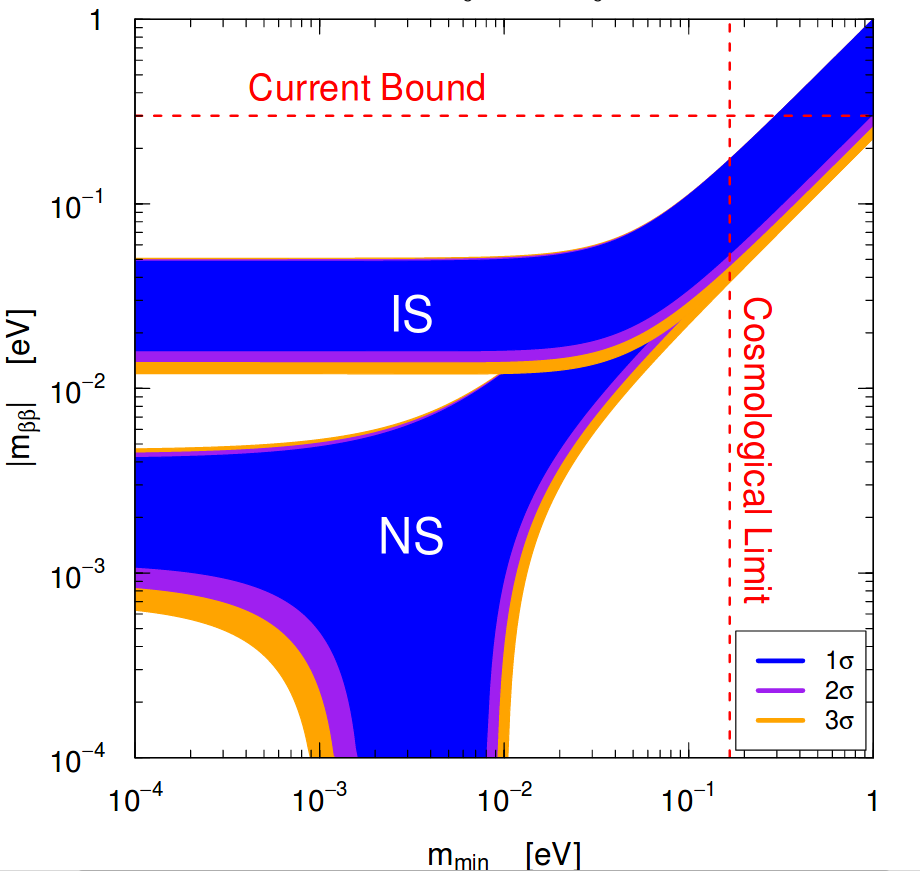
\includegraphics[width=\textwidth]{./Bilder/NeutrinoMassOrdering.png}
		\caption{Value of the effective neutrino mass $\left\langle m_{\beta\beta}\right\rangle$ detectable by \onbb\ as a function of the smallest mass of the respective mass hierarchy. NS stands for the normal hierarchy and IS for the inverted hierarchy. Taken from \cite{bilenky_neutrinoless_2012}.}
		\label{fig:MassOrder}
	\end{minipage}\hfill%
	\begin{minipage}{.5\textwidth}
		\centering
		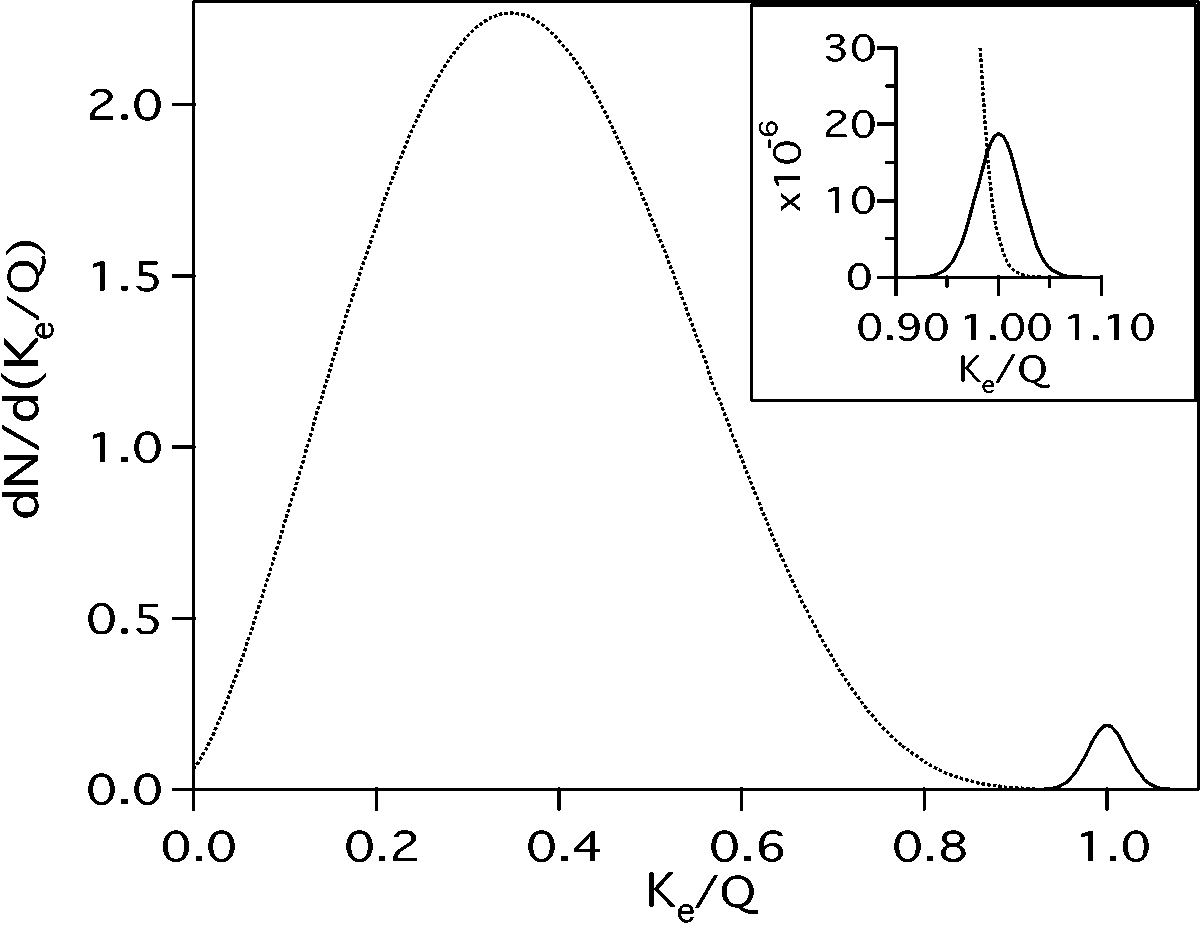
\includegraphics[width=\textwidth]{./Bilder/TheoretischesSpektrmdes0nubbDecay.png}
		\caption{Effective spectrum of a \twonu\ decay when adding the energies of the two escaping electrons. In the case a \onbb\ decay exist a peak at the Q-value of the \twonu\ decay spectrum can be seen. Taken from \cite{elliott_double_2002}.}
		\label{fig:TheoSpektrum}
	\end{minipage}
\end{figure}

\subsection{Experimental methods to detect a \onbb\ decay}

The experimental signature of the \onbb\ decay is a sharp peak at the $Q_{\beta\beta}$ value of the \twonu\ decay in the effective spectrum of the two electrons (see figure \ref{fig:TheoSpektrum}).
One experimental approach is to use a detector made of material enriched in a \onbb\ decaying isotope.
This has the advantage that the detection efficiency is maximized.
\\

Since \onbb\ decay should have a very long half-life, any background has to be minimized just to measure the resulting influence.
There are three kind of background sources that have to be considered.
\begin{enumerate}
    \item Cosmic background radiation.
Muons shower down to the earth from the atmosphere and create background in the detectors.
Their influence can be suppressed by placing the experiment deep underground and applying a muon veto system.
\item Natural radioactivity.
This is typically the dominant background source originating from radioactive isotopes which are naturally present in all materials.
Its influence can be suppressed by passively shielding the detectors and the selection of low radioactive components in the setup. 
\item The \twonu\ decay material itself.
Its impact on the background can not be reduced by external measures or shielding.
However, by using a detector with high energy resolution or a decay material of high Q-value its influence can be suppressed.
\end{enumerate}
\\

\nuc{Ge}{76} is often used in \onbb\ decay search experiment. 
Due to it being a semiconductor it can be used as the detector material itself.
A disadvantage of \nuc{Ge}{76} is its low Q-value of $Q_{\beta\beta} = 2039\unit{keV}$, which is lower than \nuc {Tl}{208}'s and \nuc{Bi}{214}'s end point energy.
It is also hard to increase the target volume compared to e.g. \nuc{Xe}{136}.
Its advantage, however, is its ability to be made with great intrinsic radio-purity, its high energy resolution and its high detection efficiency.
These facts outweigh the disadvantages which is why it already has a long history for being used as decay material and why it was chosen for the \gerda\ experiment.
\\

%\nuc{Ge}{76} has a long history of use as decay material in \onbb\ experiments, most notably in the Heidelberg-Moscow(HdM) and the IGEX experiments.
%Both of these experiments are the predecessor experiments of \gerda\.
%With detectors made of enriched germanium plus the background reducing precautions and active vetos described above they were able to set a similar limit of the half life of the \onbb\ to $\thalfzero(\nuc{Ge}{76}) > 1.9\times10^{25}\unit{yr}$ \cite{noauthor_phys._nodate}. 
%HdM experiment actually claimed to have measured the half life of about $\thalfzero(\nuc{Ge}{76}) = 1.19\times10^{25}\unit{yr}$ , but its legitimacy has been questioned by a part of the scientific community \cite{klapdor-kleingrothaus_search_2004}.
%\\

%This is where the  \gerda\ experiment comes in.
%Its first measuring phase (\PI) was planned to verify or falsify the results of the HdM experiment using the detectors used in the HdM and the IGEX experiment.
%\PI started in November 2011 and May 2013 with a total exposure  of  $21.6 \frac{\unit{kg}}{\unit{yr}}$ and no signal of a \onbb\ observed \cite{agostini_results_2013}.
%With its results and the results from HdM and IGEX a new lower limit for the half life was able to be set at $\thalfzero(\nuc{Ge}{76})>3.0\times10^{25}$  yr  (90$\%$ C.L.)
%The second phase (\PII) with 30 new custom-made enriched detectors together with the old detectors has started measuring in late 2015 and had its latest data published !!!! hier noch ob ich das NATURE paper quoten soll!!!!!.
%A more detailed description of the construction and functionality of the \gerda\  \PII~ is the topic of the next section.

% also a bit about standard double beta decay
% differences between the standard and neutrinoless beta decay
 


\section{\gerda\ \PII}
\label{sec:gerda}

% general Information, e.g. 
% sizes 
% Gran Sasso, 
% what other  neutrino less beta decay experiments are there,

\subsection{Experimental Setup}
\label{sec:ExSetup}
The \gerda\ experiment is located in the underground Laboratori Nazionali del Gran Sasso (LNGS) of INFN, Italy.
The laboratories are located approx. 1.4 km below ground, which corresponds to a water equivalent of 3.5km.
\gerda\ experiment uses \nuc{Ge}{76} as \onbb\ decay material as well as the detector material \cite{agostini_background_2017}.
\\

The detectors are operated bare in a liquid argon (LAr) tank of 64m$^3$ volume at an working temperature of about 90K.
Its main purpose is to cool the germanium detectors down to their working temperatures and to passivly shield against external radiation originating from the outside.
LAr can also scintillate.
That is why in \PII\ extra instrumentation was positioned inside the LAr tank the measure any light signal around the detectors.
Because any \nuc{Ge}{76} decays are unlikely to create scintillation light their signal can be used as a veto - the so called LAr veto.
\\

Situated around the LAr is a 590m$^3$ water tank.
Its main purpose is to shield the setup from outside radiation not only passively by absorption but also actively as a muon veto.
Situated in the water tank are 66 photomultipliers.
These detect any Cherenkov light created mostly by Muons.
Again, \nuc{Ge}{76}'s Q-value is to low to create any kind of Cherenkov light which is why any light signal can be used as a veto.

Over the water tank is a clean room situated in which the detector strings can be assembled into the strings.  
The general setup can be seen in figure \ref{fig:gerdaSetupPII}.
\\

\begin{figure}[t!]
	\centering
	\begin{minipage}[t!]{.45\textwidth}
		\centering
		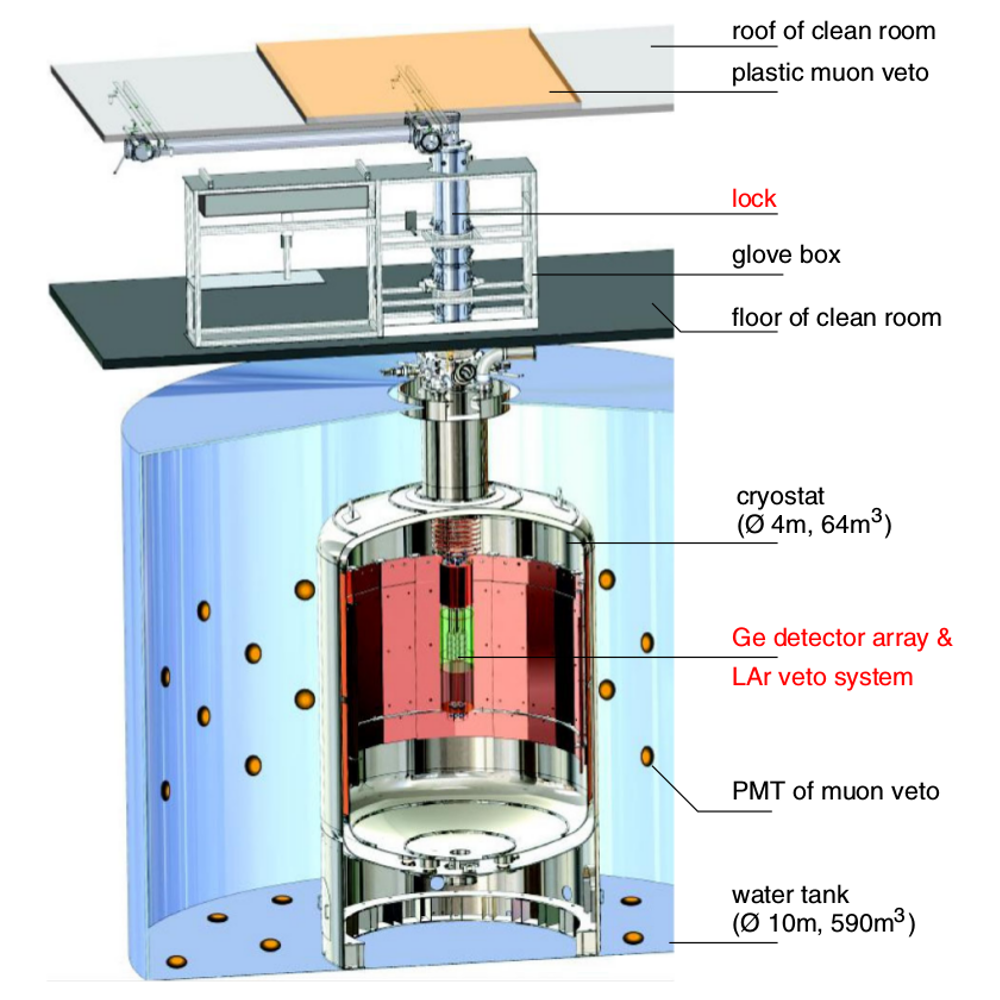
\includegraphics[height=60mm]{./Bilder/GERDAsetupPhaseII.png}
		\caption{Sketch of the \gerda\ \PII\'s experimental setup. The germanium source and detectors are placed inside a liquid argon (LAr) tank which itself is surrounded by a water tank. Taken from \cite{collaboration_upgrade_2018}.}
		\label{fig:gerdaSetupPII}
	\end{minipage}\hfill%
	\begin{minipage}[t!]{.45\textwidth}
		\centering
		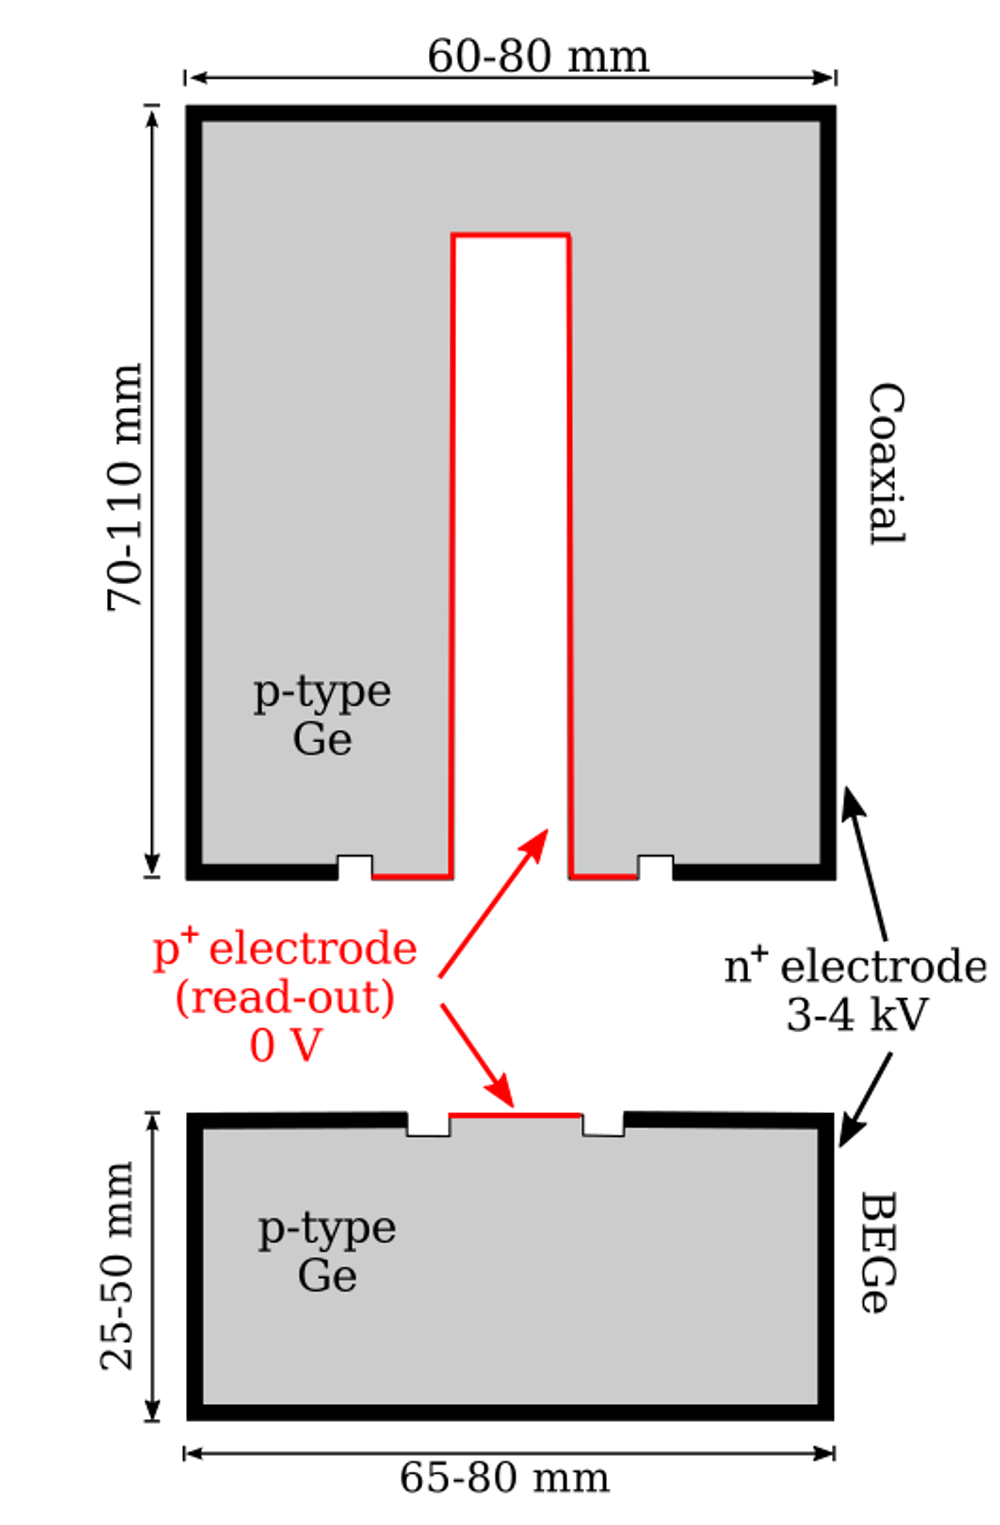
\includegraphics[height=60mm]{./Bilder/DetectorDesign.png}
		\caption{Sketch of the Coaxial (COAX) and Broad Energy Germanium (BEGe) detector designs. The COAX detectors have are larger and have a cylindrical coaxial cavity while the BEGes are completely solid. Taken from \cite{agostini_background_2014}.}
		\label{fig:DetcDes}
	\end{minipage}
\end{figure}

Now to the detectors themselves.
\gerda\ \PII~ uses seven coaxial detectors (COAX) that have already been used in the predecessor experiments HdM and the IGEX as well as 30 new Broad Energy Germanium detectors (BEGe).
Both of these detector types are made of germanium that has been enriched from 7.8$\%$ of \nuc{Ge}{76} to about 87$\%$ \cite{agostini_background_2017}.
They also share the same basic functionality.
The major volume of both detectors are made of p-type germanium.
Both detectors have the majority of their surface covered by a 1-2mm thick n$^+$ doped electrode and only a small part with an p$^+$ electrode.
If an electron hole pair is created in the p doped area, the charged particles are separated and guided to the n$^+$ or the p$^+$ layer respectively by a strong electrostatic field (3 to 4 kV) between the electrodes  \cite{spieler_semiconductor_2005}.
If the pair is created in the n$^+$ layer the hole is most likely to recombine in the $n^+$ layer due to its low mobility and therefore creates no measurable signal.
The n$^+$ layer is therefore not not active and called a dead layer.
\\

The two detectors however differ in their design as seen in figure \ref{fig:DetcDes}
But the detector types also differ in their mass and therefore their expected exposure per detector and energy resolution.
The COAX detectors are generally heavier and therefore have a higher detector efficiency then the BEGe.
But their design also results in a worse energy resolution due to their higher capacity compared to the BEGes \cite{agostini_production_2015}.
BEGes also allow for a better pulse shape discrimination (PDS) compared to the COAX detectors \cite{agostini_pulse_2013}.
PDS can make a statement about the creation process of the electron hole pair by looking at the shape of the signal.
It can therefore discriminate between different kind of origins for a signal and acts as a veto.
\\

The enriched detectors are assembled into 6 strings forming a hexagonal array together with a seventh string.
This seventh string consists of three extra coaxial detector made of natural isotopic Ge.
However they are not used in \gerda's main analysis.

Custom made amplifiers also located in the liquid argon above the detectors and digitized the analog signals of the detectors at a sampling rate of 100MHz if a triggering signal was found \cite{riboldi_cryogenic_2015}.
Every 20 seconds a charged pulse, called the test pulse, is injected into the the front-end electronics.
Its purpose is to monitor leakage current and noise \cite{agostini_background_2017}.
The analysis of the signals is performed offline.


\iffalse
\begin{figure}[t!]
	\centering
	\begin{subfigure}{.66\textwidth}
		\centering
		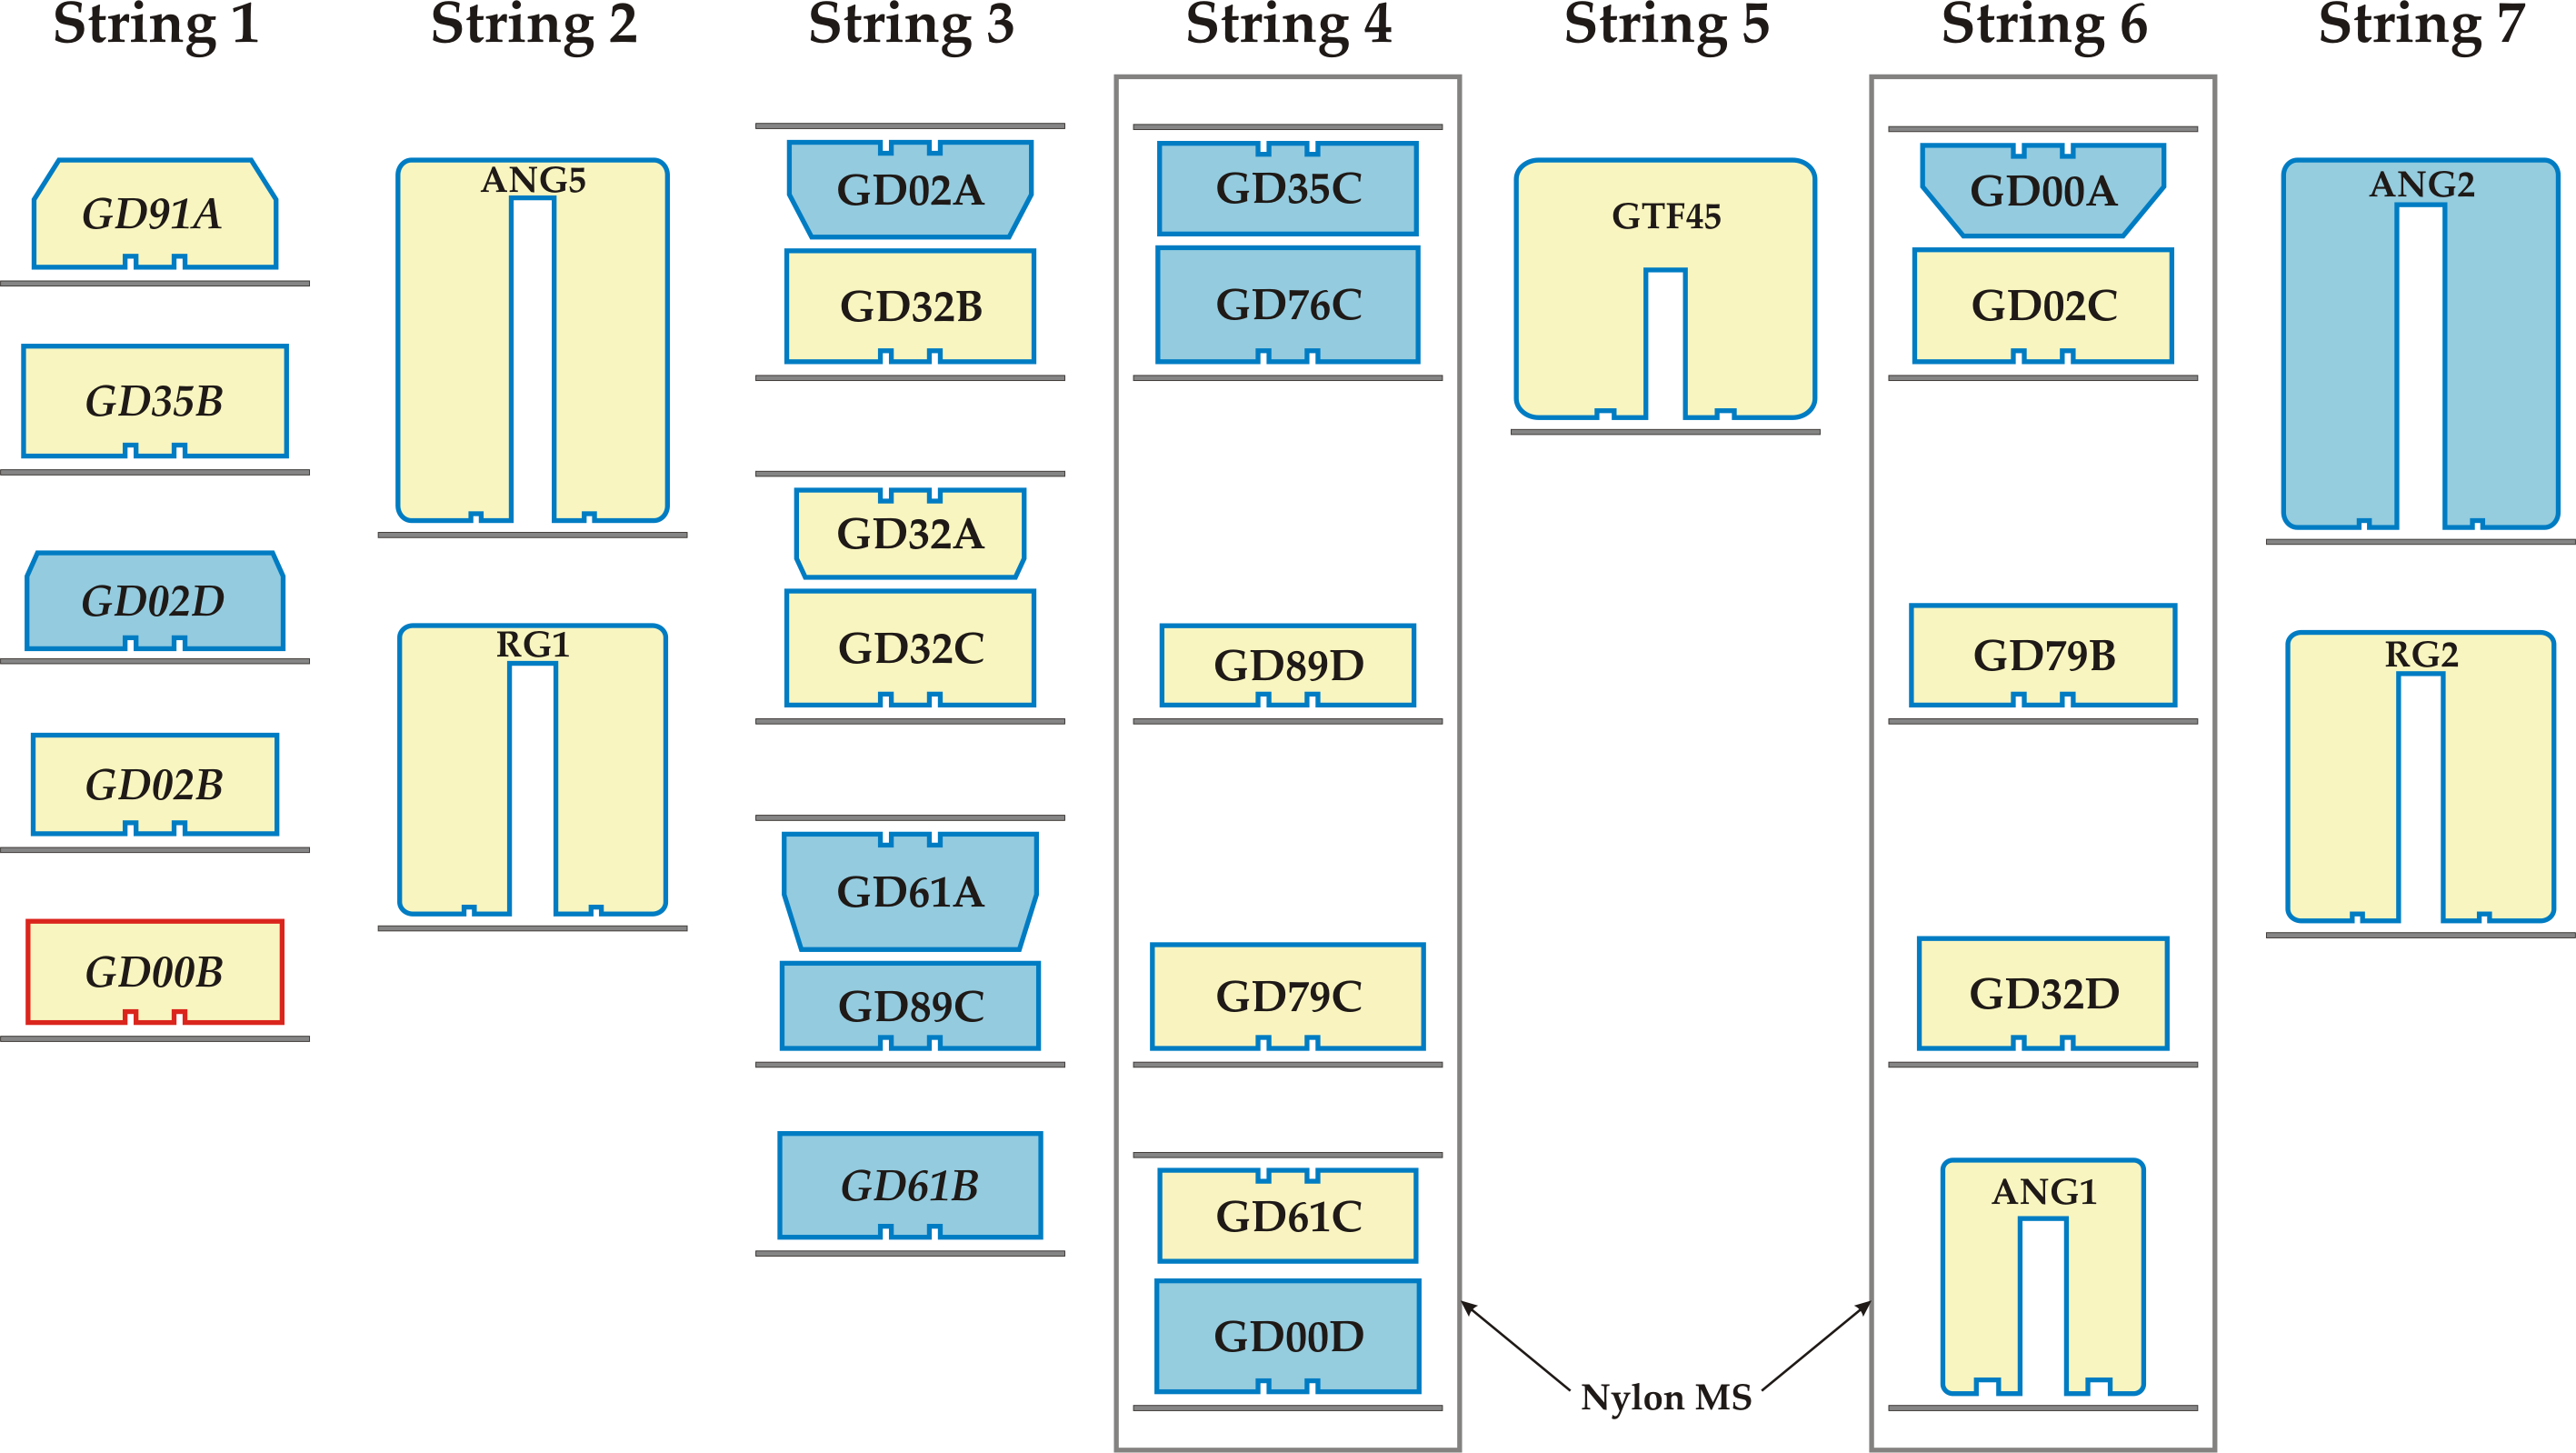
\includegraphics[width=.9\textwidth]{./Bilder/strings.png}
		\caption{}
		\label{fig:strings}
	\end{subfigure}\hfill%
	\begin{subfigure}{.30\textwidth}
		\centering
		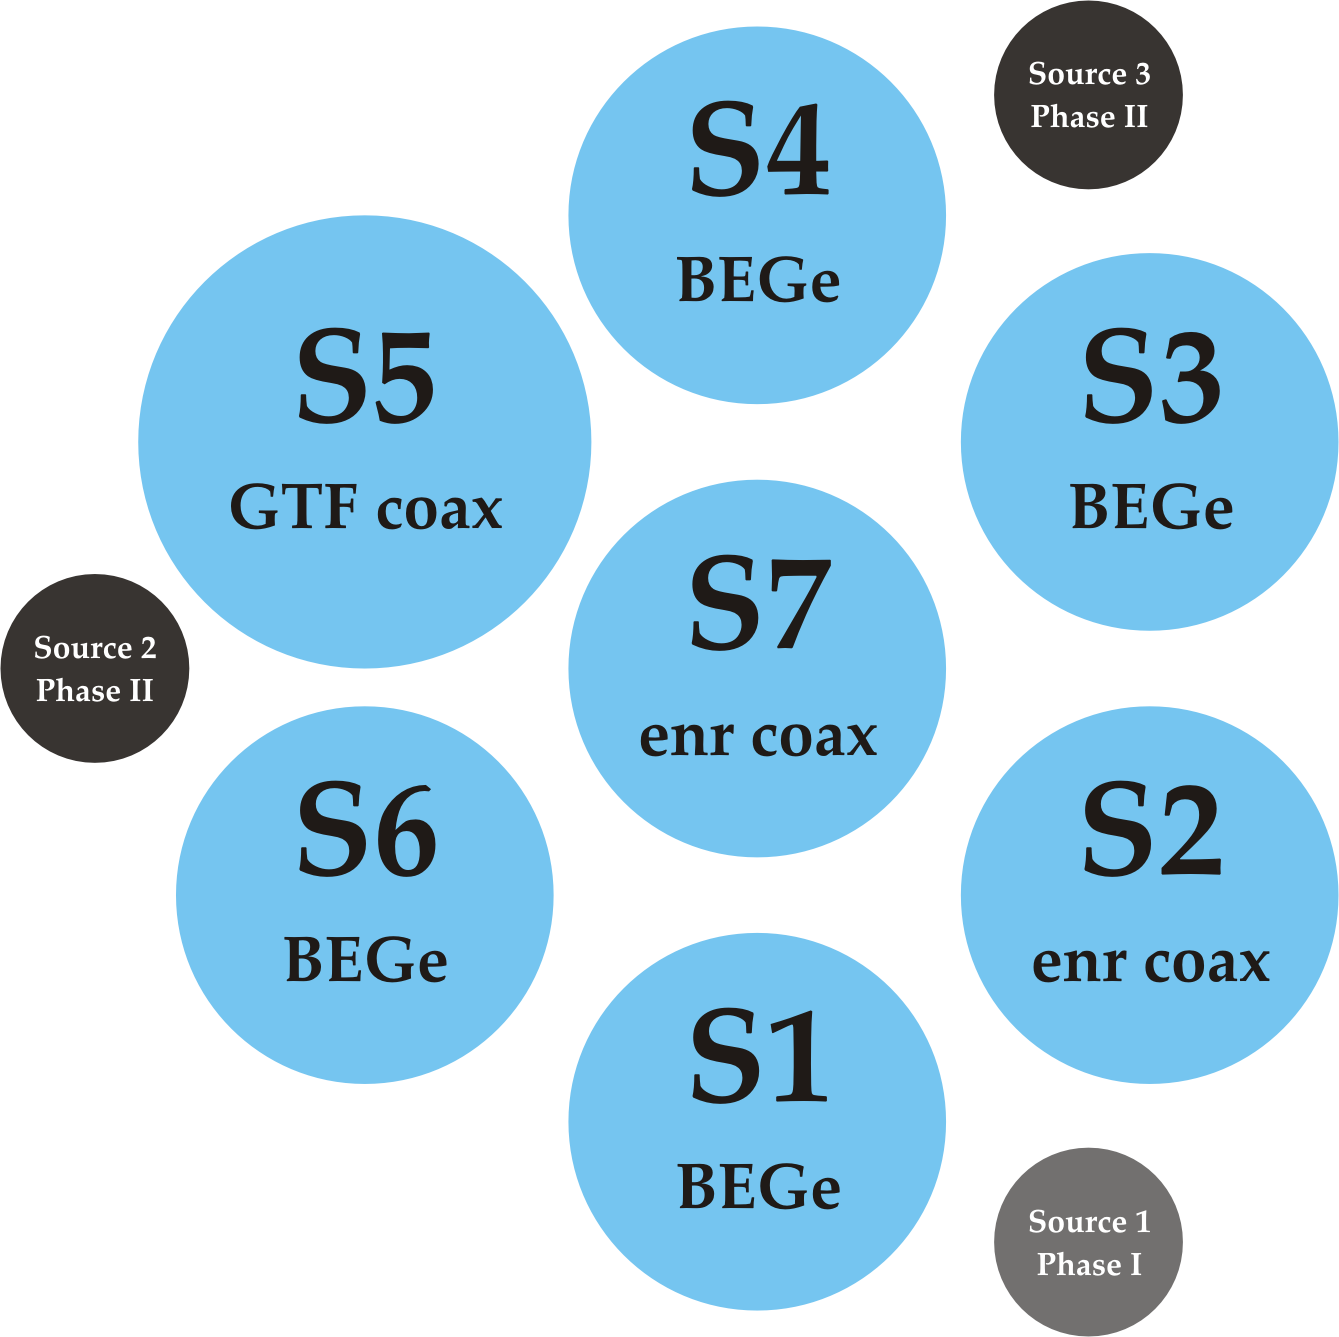
\includegraphics[width=.9\textwidth]{./Bilder/strings-top.png}
		\caption{}
		\label{fig:stringsabove}
	\end{subfigure}
\end{figure}
\fi
% well, just dump everything here
% also a bit about Tier1-4 storage of data 

Surrounding the detectors so called nylon mini shrouds (NMS) are attached to limit the amount of LAr volume around the detectors.
This is in place to passively suppresses the background created from \nuc{K}{42}.

\subsection{Liquid Argon as Coolant, Shielding and Scintillator} 
\label{sec:LArcoolant}

LAr has the property that scintillation light is produced when electrically charged radiation excites or ionizes atoms in the material \cite{olsen_improvements_nodate}.
The excited atoms in a noble liquids form dimer pairs (Ar$^*_2$).
These dimer pairs are meta stable and relax with the release of a vacuum ultraviolet photon (VUV)  which have a wavelength of 128 nm.
In the end each ionized or excited atom only produces one VUV photon.
In nobel liquids the VUV light does not have enough energy to excite any atom in the ground state allowing the VUV to have a very long travel distances of without being absorbed.
\\

\begin{figure}[t!]
	\centering
	\begin{minipage}{.475\textwidth}
		\centering
		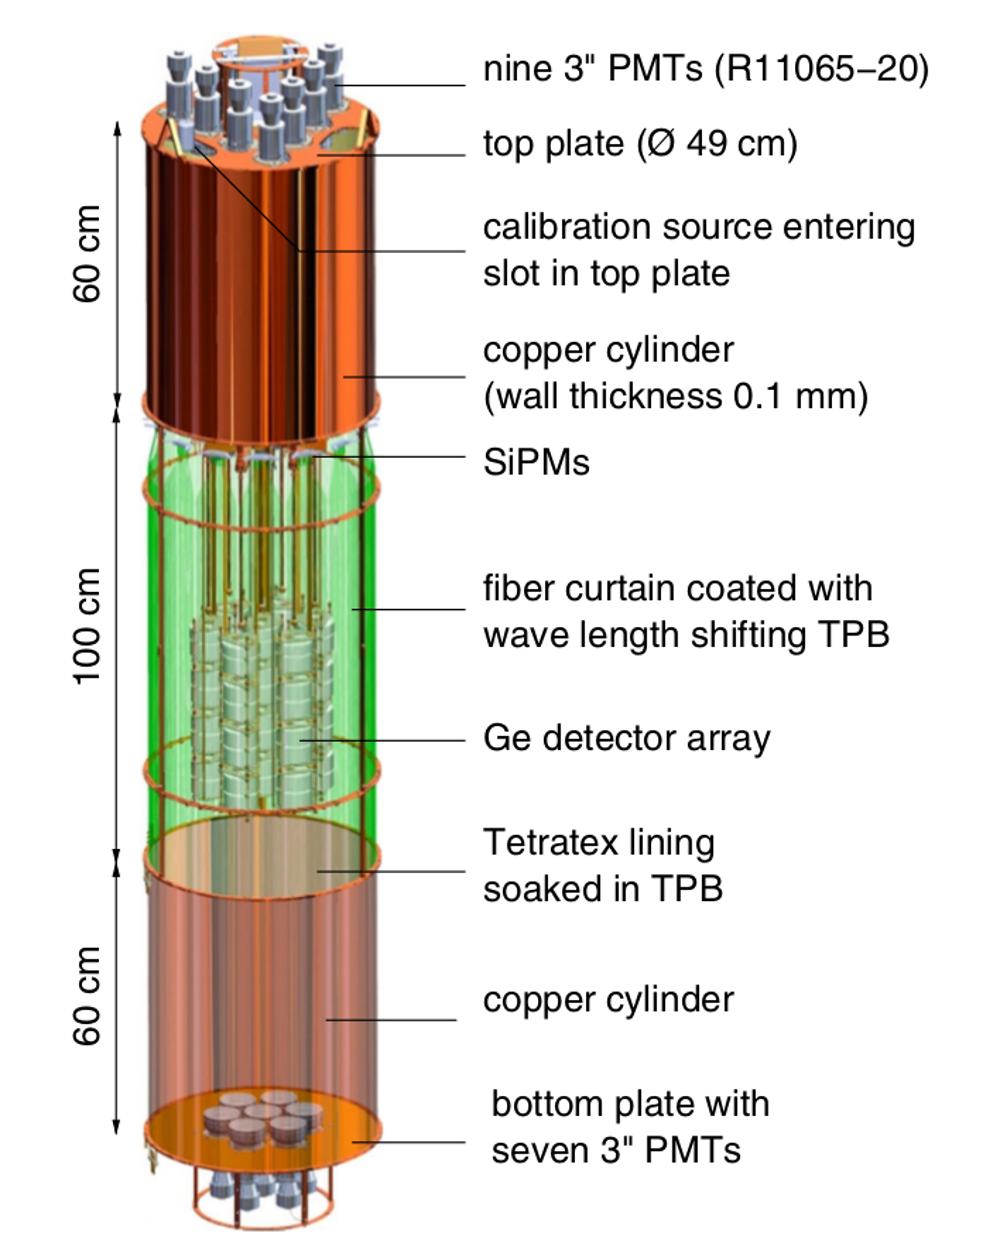
\includegraphics[width=0.6\textwidth]{./Bilder/LArVetoSetup.png}
		\caption{Sketch of the liquid agron (LAr) veto setup. 16 photomultiplier tubes (PMT) are mounted in a cylindrical copper surface at the top and bottom. At the level of the detectors instead of copper, the cylinder consists of fibers. These are read out at their ends by silicon photomultipliers (SiPM). Taken from \cite{collaboration_upgrade_2018}.}
		\label{fig:LArVetoSetup}
	\end{minipage}\hfill%
	\begin{minipage}{.475\textwidth}
		\centering
		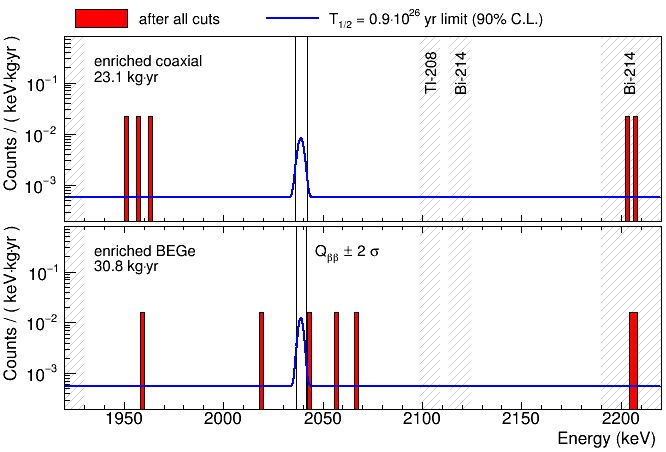
\includegraphics[width=\textwidth]{./Bilder/GerdaErgebnisse.png}
		\caption{Recent results from \gerda\ \PII. The measured spectra of COAX and BEGe detectors are distinguished by their different resolutions.  Only one decay 2 sigma from the \onbb\ decay was found. This leads to the conclusion that no \onbb\ decay was measured and a new lower limit of \thalfzero\ = $0.8\times10^{26}\unit{yr}$ (90$\%$ CL) was determined. Taken from \cite{zsigmond_new_2018}}
		\label{fig:gerdaErgebnisse}
	\end{minipage}
\end{figure}

Background events often deposit energy in the argon while passing through it.
Their scintillation light around the detectors can therefore be used as a veto to reject those events.
That is why a cylindrical copper shell around the germanium detectors is equipped with 16 photomultiplier tubes (PMT), situated at the bottom and at the top of this volume.
At the level of the detectors the shell is not made of copper but of nylon strings.
These are read out by 90 silicon photomultipliers (SiPM) measuring any light signal travailing through them \cite{csathy_optical_2016} (see figure \ref{fig:LArVetoSetup}).
VUV has a wavelength so small most material absorbs it in ionization.
That is why wavelength shifting material covers the nylon fibers and the photomultipliers shifting from 128nm to 400nm.
\\

LAr is also a good coolant due to the characteristically low melting point of nobel gases.
In \gerda\ it is cooled down to the working temperature of the germanium detectors at about 90 K.

Nobel liquids are also great as ultra radio-pure passive shielding.
This is because noble elements rarely make any chemical bonds due to their fully filled electron shells.
It is therefore possible to filter the majority of impurity just by distillation.
Compared to other noble gases argon also has the advantage of a very low price due to it being easily obtained by liquefaction of air from the atmosphere.
\\




\subsection{Data processing and analysis}
\label{sec:DataProc}

\label{sec:Resultsofgerda}
\begin{figure}[t!]
	\centering
		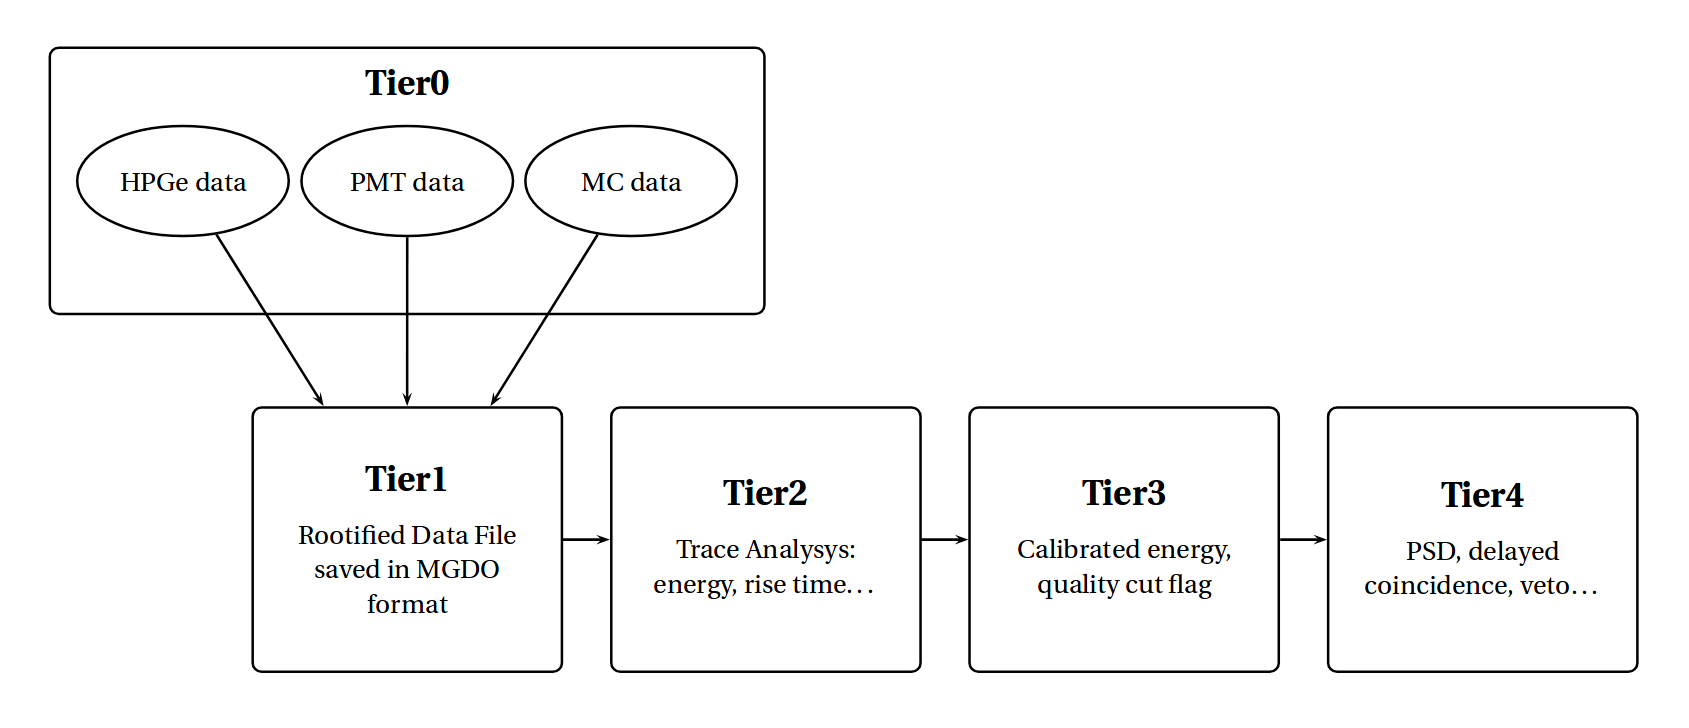
\includegraphics[width=100mm]{./Bilder/TierStructure.png}
		\caption{The multi-tier structure used by GELATIO. Tier0 and Tier1 contain all of the raw data. However, the data in Tier1 has already been converted to root files. Tier2, Tier3 and Tier4 store  progressively more analyzed data. Taken from \cite{agostini_gelatio:_2011}}
		\label{fig:TierStructure}
\end{figure}

As already mentioned, in the case of an event the digitized signals of the germanium detectors and the photomultipliers are stored for further offline analysis.
The software used for this purpose is \gerda\ LAyouT for Input/Output (GELATIO).
It is a data analysis framework suitable for off-line digital signal processing and analysis of data recorded by germanium detectors.
It's advantages are its multiple level data organization and its modular digital signal processing.
These two points leave the analysis protocol incredibly flexible.
\\

The multi-tier structure used in GELATIO can be seen in figure \ref{fig:TierStructure}.
Tier0 and Tier1 store raw information while all higher Tiers contain progressively more analyzed data.
Additional information about the analysis process can be found in \cite{agostini_gelatio:_2011} and \cite{agostini_off-line_2011}.
In this thesis only data from Tier3 and Tier4 will be used.
\\

To ensure that the filter parameters of the analysis are set without bias, all events measured in a  50 keV interval around the $Q_{\beta\beta}$ were only stored without any analysis applied on them.
Only after all parameters in the rejection process were finally defined all events from this interval will be analyzed. 
Such a procedure is called a blinding process and the revealing of the blinded events an unblinding. 
\\
% Mui, Mountain, Pulse shape disc.
% especially LAr-Veto 

\subsection{Recent Results}

\begin{figure}	
		\centering
	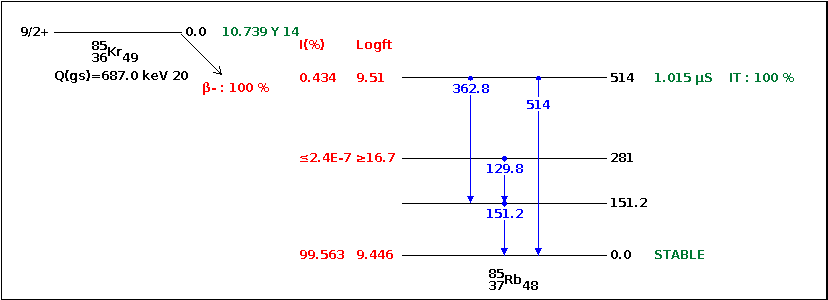
\includegraphics[width=\textwidth]{./Bilder/Kr85Decay.png}
	
	\caption{
	The decay scheme of \Kr. It decays via two different channels. The majority of transitions end in the ground state of \nuc{Rb}{85} while 0.434$\%$ of the times \Kr decays into a excited state being 514 keV over the ground state. The excited state has a half life of 1.015$\mu$s. It then relaxes directly into the ground state. Taken from \cite{noauthor_livechart_nodate}.
	}
	\label{fig:Decay}
\end{figure}
Only recently new data was published by \gerda\ \cite{zsigmond_new_2018}.
In it only one event in the proximity of the Q-value was found as seen in figure \ref{fig:gerdaErgebnisse}.
However, more than 2 sigma from the expected peak position.
The conclusion was therefore that no evidence for a \onbb\ decay has been seen.
A new lower limit for \nuc{Ge}{76} was determined to be $\thalfzero\ = 0.9\times10^{26}\unit{yr}$ (90$\%$ CL).
Currently \gerda\ receives an upgrade and is planned to measured for until 2020.
After that the successor experiment LEGEND is planned to investigate the lower limit of \nuc{Ge}{76} half life further.

% what has happened so far

% short outline of approaches


\section{\Kr\ isotope in the atmosphere}
\label{sec:Kry85}

\Kr\ has a mass number of A = 85 and an atomic number of Z = 36.
This isotope is not stable and decays via a $\beta^-$-decay into \nuc{Rb}{85}.
The half life of this decay is 10.756 yr \cite{singh_nuclear_2014} and a Q-value of $Q_\beta = 687 \unit{keV}$.
\Kr's $\beta$-decay has two different possible transitions (see figure \ref{fig:Decay}).
With overwelming 99.563$\%$ of the times the \Kr decay has its final state in the ground state of \nuc{Rb}{85}.
In 0.434$\%$ of the times however it decays via an excited state of \nuc{Rb}{85} 514 keV above the ground state.
This excited state has a half life of 1.015 $\unit{\mu s}$ and it basically always relaxes directly into the ground state with the emission of a photon carrying their energy difference.
\\

\begin{figure}[t!]
	\centering
	\ifmakefigures%
	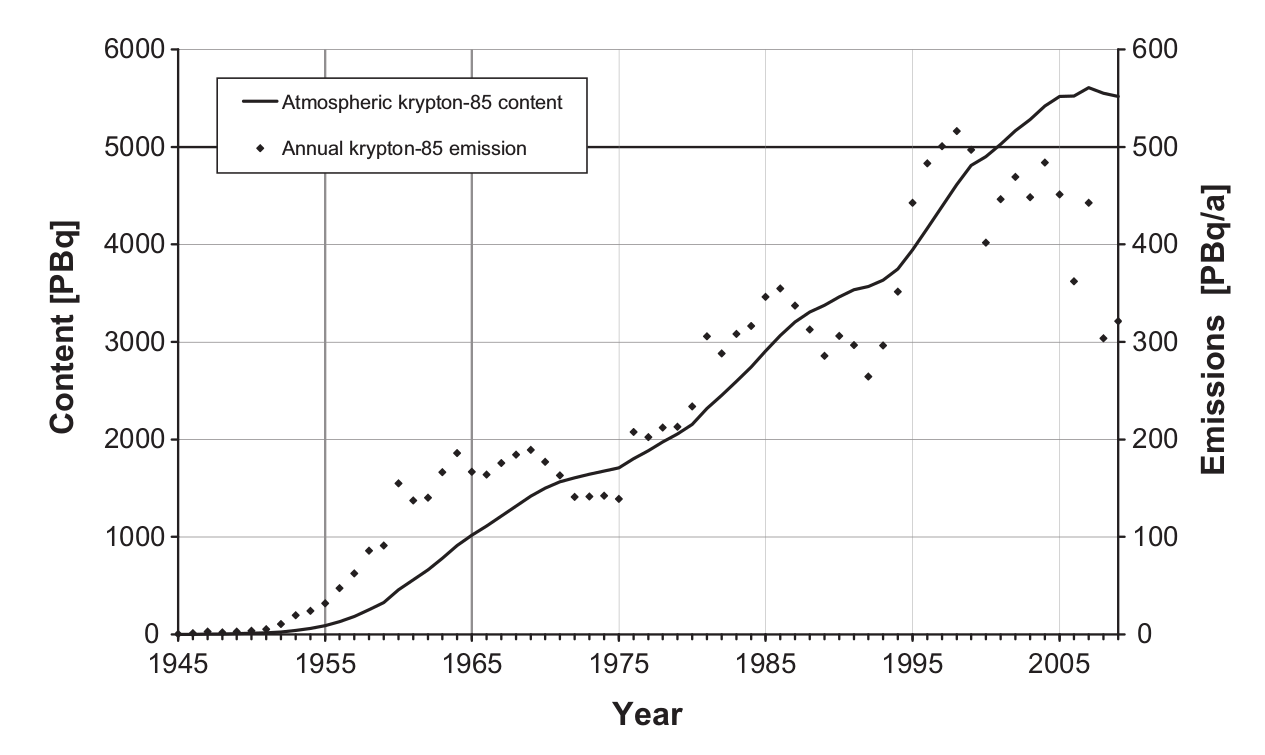
\includegraphics[width=80mm]{./Bilder/Kr85Aenderung.png}
	\fi%
	\caption{
	    \Kr's specific activity in the atmosphere from 1945 to 2009. It can be seen that over this period the average specific activity in the atmosphere has increased. This is due to the higher amount of fission reactors in which \Kr is produced.   
		Taken from \cite{ahlswede_update_2013}.
	}
    \label{fig:Kr85Aenderung}
\end{figure}


The main interest of this thesis lies with the concentration of \Kr\ in argon.
The argon used in \gerda\ \PII\ was extracted from the atmosphere.
But how did \Kr\ get there?
There are two main sources \Kr\ can be originate from on earth.
It can be created in the atmosphere naturally by an interaction of \nuc{Kr}{84} with cosmic rays.
In equilibrium this accounts to an activity of 0.09PBq in the whole atmosphere \cite{winger_new_2005}.
However, the production of \Kr\ from nuclear fission of \nuc{U}{235} and \nuc{Pu}{239} generates an atmospheric inventory about four orders of magnitude higher than that.
Only a small amount is natural produced in earth's crust.
The majority is man made from nuclear power plants.
Krypton is a noble gas and therefore easily diffuses through everything in its way until it reaches the atmosphere.
\\

The concentration of \Kr\ in the air at ground level varies depending on the proximity to a nuclear power plant \cite{weiss_mesoscale_1986}.
At atmospheric altitudes, however, the \Kr\ concentrations only varies on large length scales since \Kr rises quickly from the ground into the atmosphere, where most of it stays longer.
Different models predict that air from the northern troposphere takes up to one year to get to the southern troposphere delaying the equalization of their \Kr\ concentrations \cite{weiss_global_1992}.
Due to the higher amount of nuclear power plants build in the last half century the activity of \Kr\ in the atmosphere has risen steadily from about 1961 PBq in 1973 \cite{telegadas_atmospheric_1975} to an estimated 5500 PBq in 2009 (see figure \ref{fig:Kr85Aenderung}) \cite{ahlswede_update_2013}.
But the change over time is so small that one can assume that \Kr's concentration in the atmosphere should be in the same order of magnitude everywhere.
This means that no matter where atmospheric air for an argon extraction would be taken, its concentration in the LAr would be of the same order. 
\\

Two experiments also using LAr are the WARP and the Darkside experiment.
In both of experiments the specific activity of their residual \Kr\ was determined.
The Darkside experiment, using underground argon (UAr), has measured a specific activity of \((2.86\pm0.18) \frac{\unit{mBq}} {\unit{l}}\)  \cite{agnes_results_2016}.
This UAr has been extracted from underground reservoirs and should only have come into contact with \Kr\ from natural processes.
Therefore its specific  \Kr\ activity should be very low. 
In the LAr of the WARP experiment a specific activity of   \((160\pm130)\frac{\unit{mBq}}{\unit{l}}\) was measured \cite{benetti_measurement_2006}.
Like GERDA it uses atmospheric argon which might cause the higher specific activity compared to  Darkside's.
It is therefore not unlikely that the specific \Kr\ activity in \gerda\ \PII\ would also be much higher than in the Darkside experiment.
Its concrete value is impotent when researching in the lower energy spectrum of \gerda\.
For example for a further investigation on \nuc{Ar}{39} that has a similar Q-value or the search for dark matter in the keV-scale.

% where does it come from?
% what properties does it have?
% why is it important to calculate its influence on \gerda\

 
\chapter{Line Count Rate Analysis}
\label{sec:SAfrom514}

The first and more precise method uses the 514 keV line count rate of the \Kr\ decay.
As discussed in section \ref{sec:Kry85}, \Kr\ has a small probability of 0.43\% to decay into an excited state of \nuc{Rb}{85m}. 
When \nuc{Rb}{85m} relaxes into its ground state it emits a photon of 514 keV energy.
The evolution of this line in the \gerda\ spectra allows to draw a conclusion on the amount of \Kr's caused events $N_{\mathrm{peak}}$ and therefor its activity. 
\\

Also necessary for the calculation is the efficiency of any germanium detector to fully absorb a 514 keV gamma.
This detector efficiency has to be determined using a Monte Carlo simulation in which an amount $N_{\mathrm{sim}}$ of  514 keV gammas were simulated in a  volume $V_{\mathrm{sim}}$.
The detector efficiency can then be calculated by dividing the simulated line count at 514 keV by the total number of  decays ($\epsilon = \frac{\Delta N}{N_{\mathrm{sim}}}$).
The value $\frac{1}{p \epsilon V_{\mathrm{sim}}}$, using the detector efficiency, the simulated volume $V_{\mathrm{sim}}$ and the probability $p$ of \Kr\ to decay via the excited \nuc{Rb}{85m}, is then a conversion factor from a measured line counts to the density of decays necessary to create this signal.
\\

The final value needed is the measuring time $\bar{t}$.
Not every detector was measuring over the course of Phase II which is why a mean measuring time for all detectors has to be calculated.
With these three values, a mean specific activity $\bar{a}$ can be determined:

\begin{equation}
    \bar{a} = N_{\mathrm{peak}}\times\frac{1}{p \epsilon V_{\mathrm{sim}}}\times\frac{1}{\bar{t}}
    \label{equ:activityDieErste}
\end{equation}The line count rate analysis is expected to generate a relatively precise estimation of the specific activity due to the 514 keV line being a clear feature that can be traced back only to \Kr.
\\

\iffalse
However, a problem of this method lies with the proximity of the \Kr\ to the 511keV peak of the positron electron annihilation. 
Its peak in the energy spectrum is expected to partially dominate over \Kr\ and does not allow for a direct measurement of the 514keV peak. 
This is not necessarily a great setback because one can just adapt the fit function to a double Gaussian peak function.
It is of interest, however, whether it is possible to completely suppers the annihilation peak without changing the 514keV photon line count.
For this one could consider using the LAr veto.
Due to the low mean energy of the escaping electron (47.65keV) of this decay, it is very unlikely that it creates any scintillating light. 
On the other hand one can expect the light of the positron electron annihilation to create a great signal in the photomultipliers.
Therefore it should be possible with the LAr veto to single out the 514keV photon events from the annihilation events.
If possible its value can be used as a cross-check for the value determined from the not filtered spectrum.

The rest of the chapter will cover the concrete implementation of the individual steps in their own sections.
\\
\fi
\section{Preparing the spectrum}

To determine the amount of measured 514keV gammas a fit has to be applied onto the corresponding line.
The data used in this analysis is the full available \gerda\ \PII\ data at the time (run 53 to 92).
Onto the events used the standard \gerda\ analysis cuts where applied.
This includes data quality cuts, the Muon veto cut and the anti-coincidence between germanium detectors of the array.
The second veto can not be triggered from \Kr\  because the measured gammas basically always happen in close vicinity of the detectors and with a $Q_\beta$ value of 687 keV it is impossible for the escaping electron to create any Cerenkov radiation.
The third veto also does not effect gamma events as they deposit all their energy in only one detector and any event with several detectors measuring a signal are likely to be background.  
\\

The data was also split for the two detector types in \gerda.
This is necessary due to the differences in detector efficiency and resolution already mentioned in seciton \ref{sec:ExSetup}.
BEGes have a lower efficiency to detect full 514 keV gammas but show a higher energy resolution ($\Delta E_{\mathrm{BEGe}} = 2.267\unit{keV}  @ 514 \unit{keV}$) and vice versa for the COAX detectors ($\Delta E_{\mathrm{COAX}} = 2.720\unit{keV} @ 514 \unit{keV}$).
Over the time investigated time frame of \PII\ all BEGe detectors were exposed to 30.836 kg$\cdot$yr and all COAX were exposed to 28.088 kg$\cdot$yr.
Some plots or examples for the COAX detectors were neglected in the course of the analysis.
This was chosen to suppress repetitiveness in the structure of this thesis due to almost identical results.
\\

\begin{figure}[t!]
\centering
\begin{subfigure}{.475\textwidth}
  \centering
	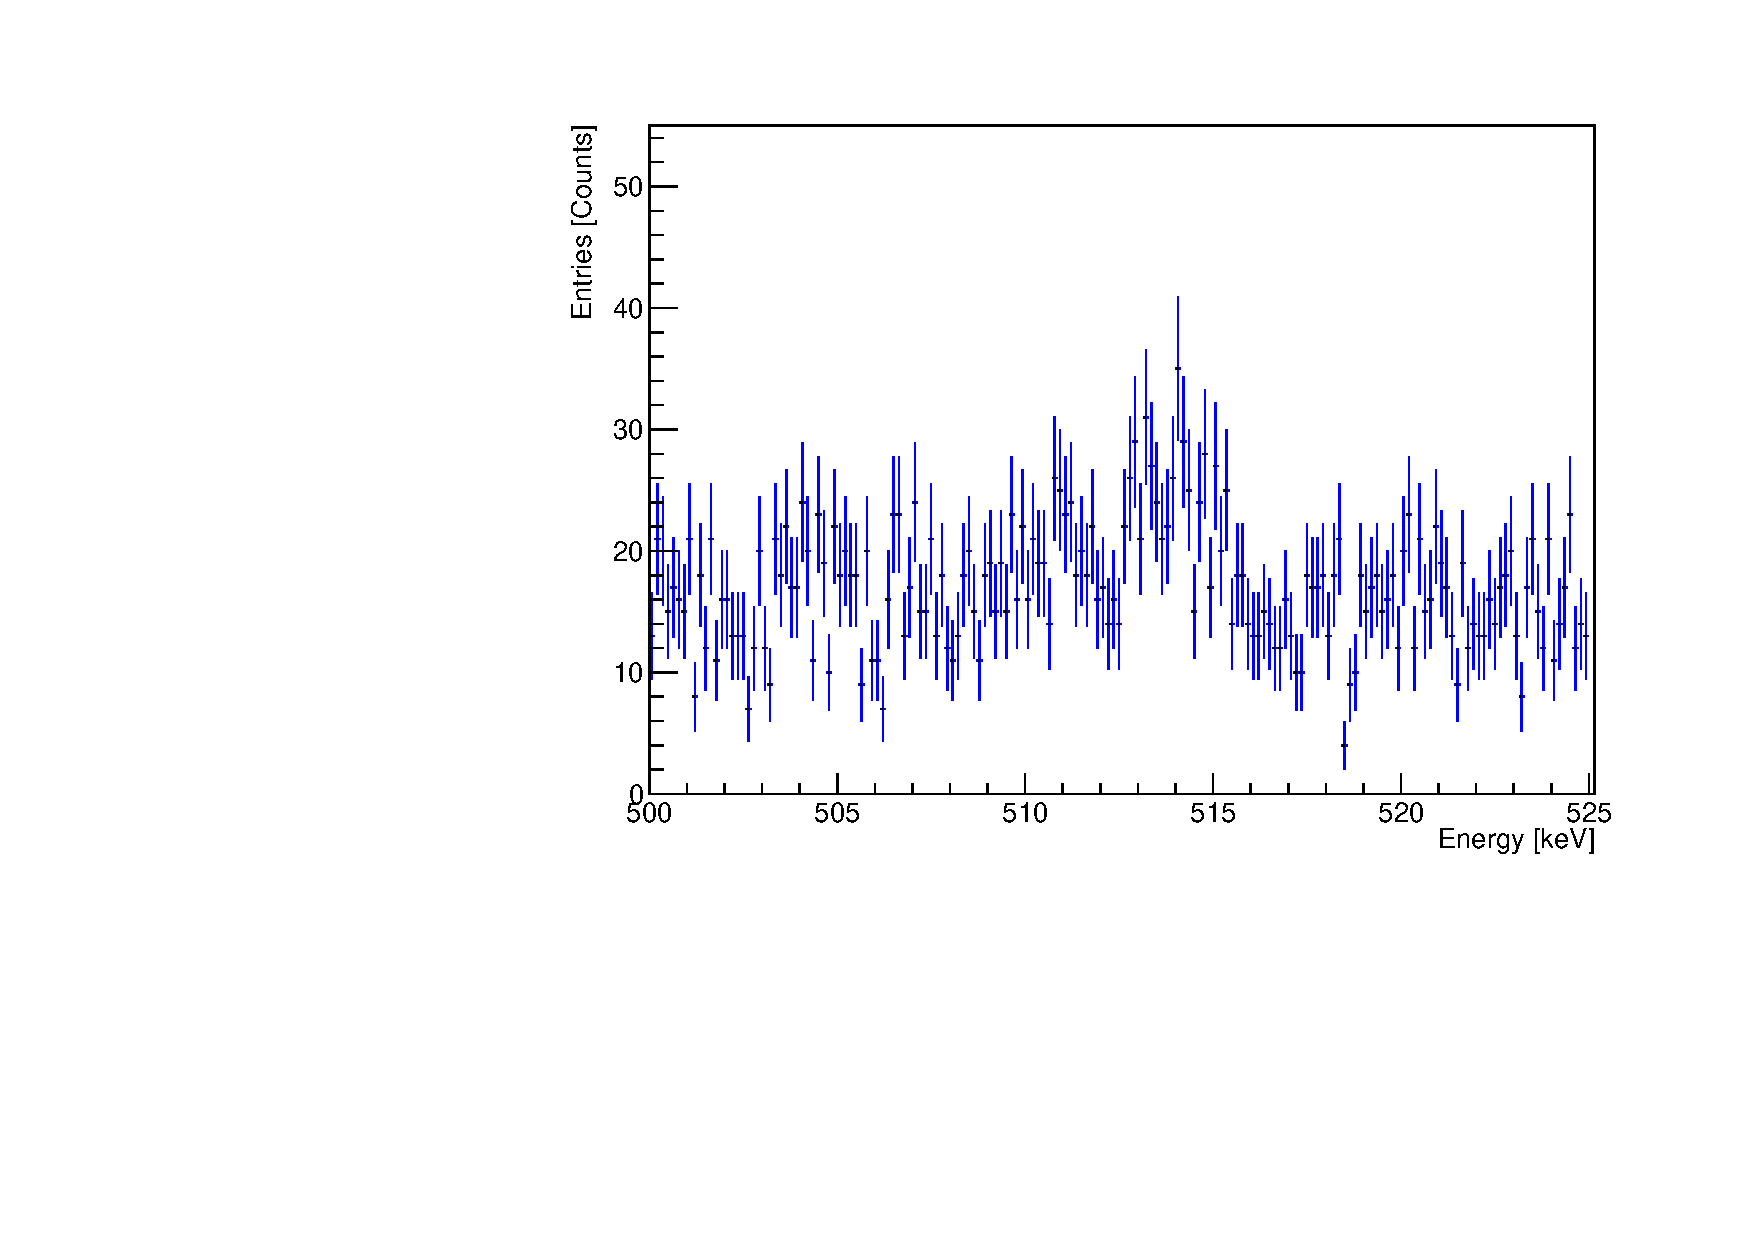
\includegraphics[width=75mm]{./Bilder/500525NoFilterBEGes.pdf}

  \caption{BEGe}
    \label{fig:NoFilterBEGes}
\end{subfigure}\hfill%
\begin{subfigure}{.475\textwidth}
  \centering
	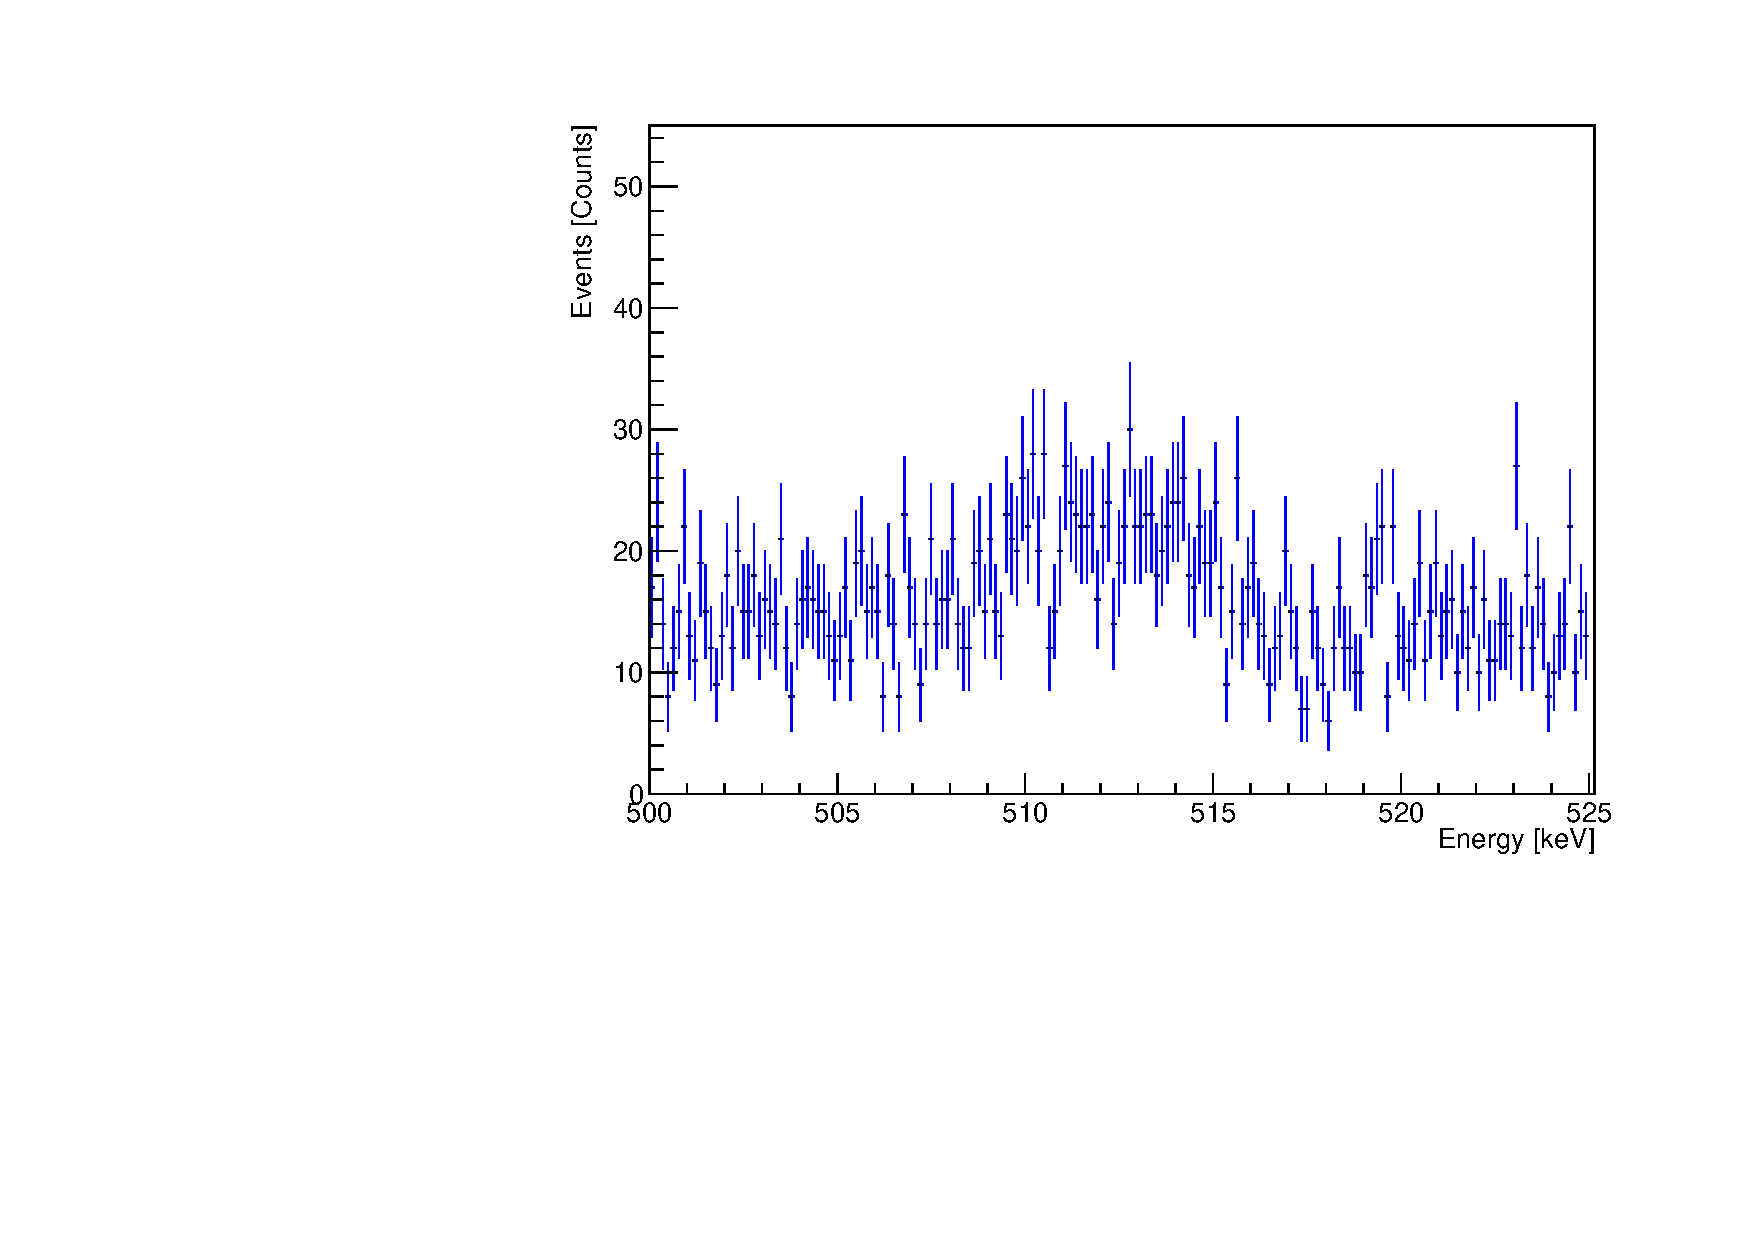
\includegraphics[width=75mm]{./Bilder/500525NoFilterCOAX.pdf}
  \caption{COAX}
  \label{fig:NoFilterCOAX}
\end{subfigure}
	\caption{Energy spectra from 500 to 525 keV after standard \gerda\ analysis cuts, split by the respective detectors the signal was measured in.}
\end{figure}

In figure \ref{fig:NoFilterBEGes} and \ref{fig:NoFilterCOAX} two resulting spectra from 500 to 525 keV of the respective detectors can be seen.
In them a structure at the 511 keV and the 514 keV line can be identified.
The 511 keV line originates from measured gammas created in positron electron annihilation events while the 514 keV line can only originate from the \Kr\ gammas.
From this one can already make the statement that a non negligible amount of \Kr\ must be present in the LAr.
Otherwise no variation from the background level should be visible.
\\

\iffalse
After the adjusting the spectra to a lower background level, one can now determine more precisely the number of measured events in the 514keV peaks of the corresponding detectors (see figure \ref{fig:NoFilterBEGes} for the BEGe and \ref{fig:NoFilterCOAX} for the spectra of the COAX detectors). 
In these two spectra one can see two peaks - one at 511keV that corresponds to the positron electron annihilation events and one at 514keV that corresponds to the photons from the relaxation of \nuc{Rb}{85m}.
From this we can already claim that there must be a non negligible amount of \Kr\ in the liquid argon.
Otherwise no peak should have been able to be measured. 
The difference in resolution as discussed above can be seen in the fact that in the BEGe diagram the two peaks have a smaller full width at half maximum (FWHM).
Compared to the COAX detectors their peaks can easily be distinguished.  
\fi




\iffalse
Another possible approach suppress the annihilation peak using an almost ideal filter and fit the resulting one peak spectrum with the original fit function.
As mentioned above the LAr Veto should be a good candidate for such a filter.

In this thesis both approaches will be applied separately and later their results compared.
Hopefully both will end up delivering the same result as no \Kr\ caused event should make a notable light signal.
But this probability is not zero which is why some events of the 514keV peak might also trigger the veto.
This would result in a smaller peak amplitude and with it a lower specific activity than the actual value. 
Whether or not a rejection process using the LAr veto would be useful in this analysis or not is the topic of the following section.
\\
\fi

\section{Annihilation Peak Suppression}
\label{sec:APS}

Because of the 511 keV peak two different approaches are now possible.
One approach would directly apply a double Gaussian peak fit function to the spectra also fitting the 511 keV peak.
Another approach would try to suppress the 511 keV peak and fit a single peak function through the spectra.
Both of these approaches will be applied in this thesis.
The first method does not need any more preparation while method needs to find an appropriate filter. 
\\

A promising candidate for this is the LAr veto.
This veto is always triggered in the case an event in the Germanium detectors coincides with a scintillation signal of at least about 0.5 phe \cite{agostini_background_2017}.
The \Kr\ decay into the excited \nuc{Rb}{85m} leaves the escaping electron with a maximum of 173 keV which should only create a very weak scintillation light signal.
Any positron creating process, however, should also create a strong scintillation light signal visible to the LAr veto setup.
This way one might be able to discriminate between \Kr\ gamma events and annihilating events.
\\

In figure \ref{fig:LArBEGes} and \ref{fig:LArCOAX} are the energy spectra from 500 to 525 keV after the LAr veto displayed.
In them one can see that the annihilation peak is reduced compare to the spectra befor the LAr veto.
\\

\begin{figure}[t!]
\centering
\begin{subfigure}{0.475\textwidth}
	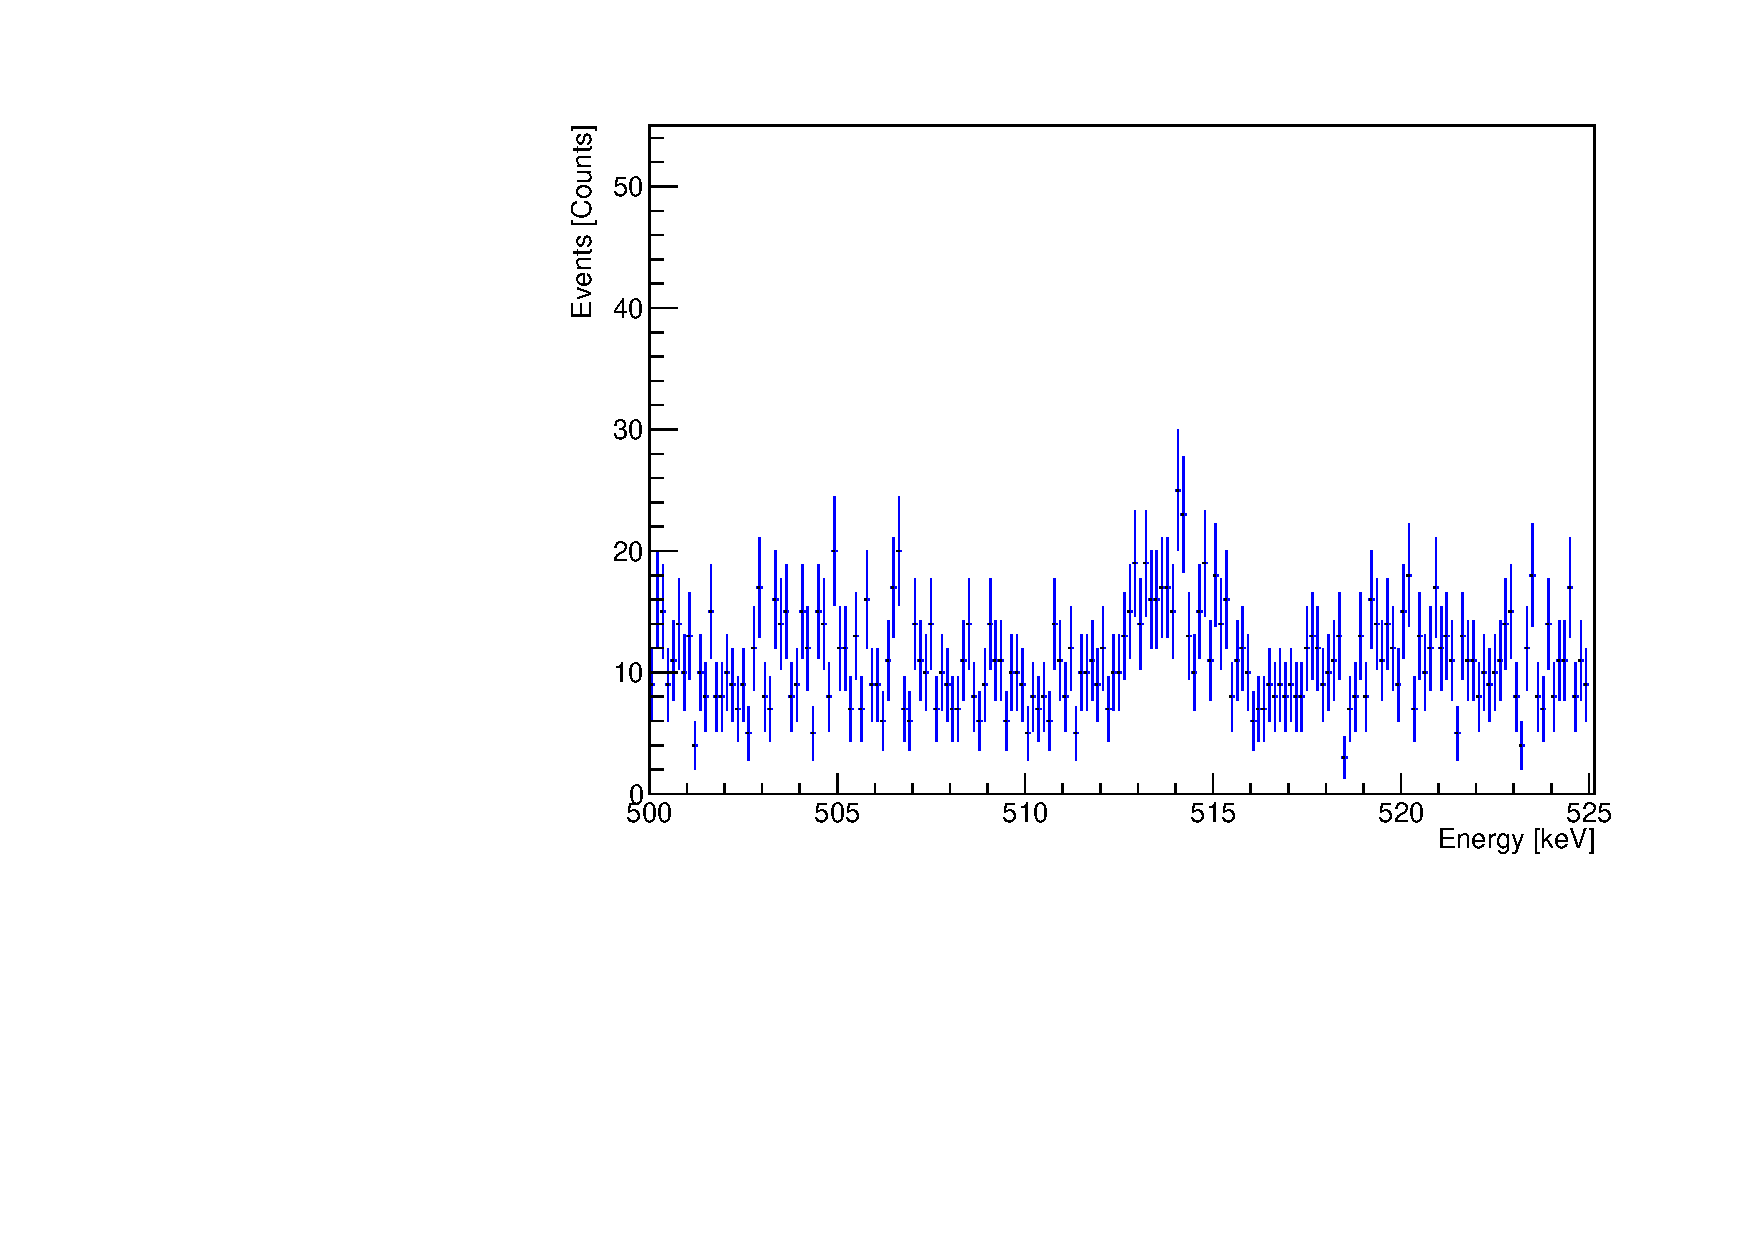
\includegraphics[width=75mm]{./Bilder/500525LArVetoBEGes.pdf}
    \caption{BEGes}
  \label{fig:LArBEGes}
\end{subfigure}\hfill%
\begin{subfigure}{0.475\textwidth}
	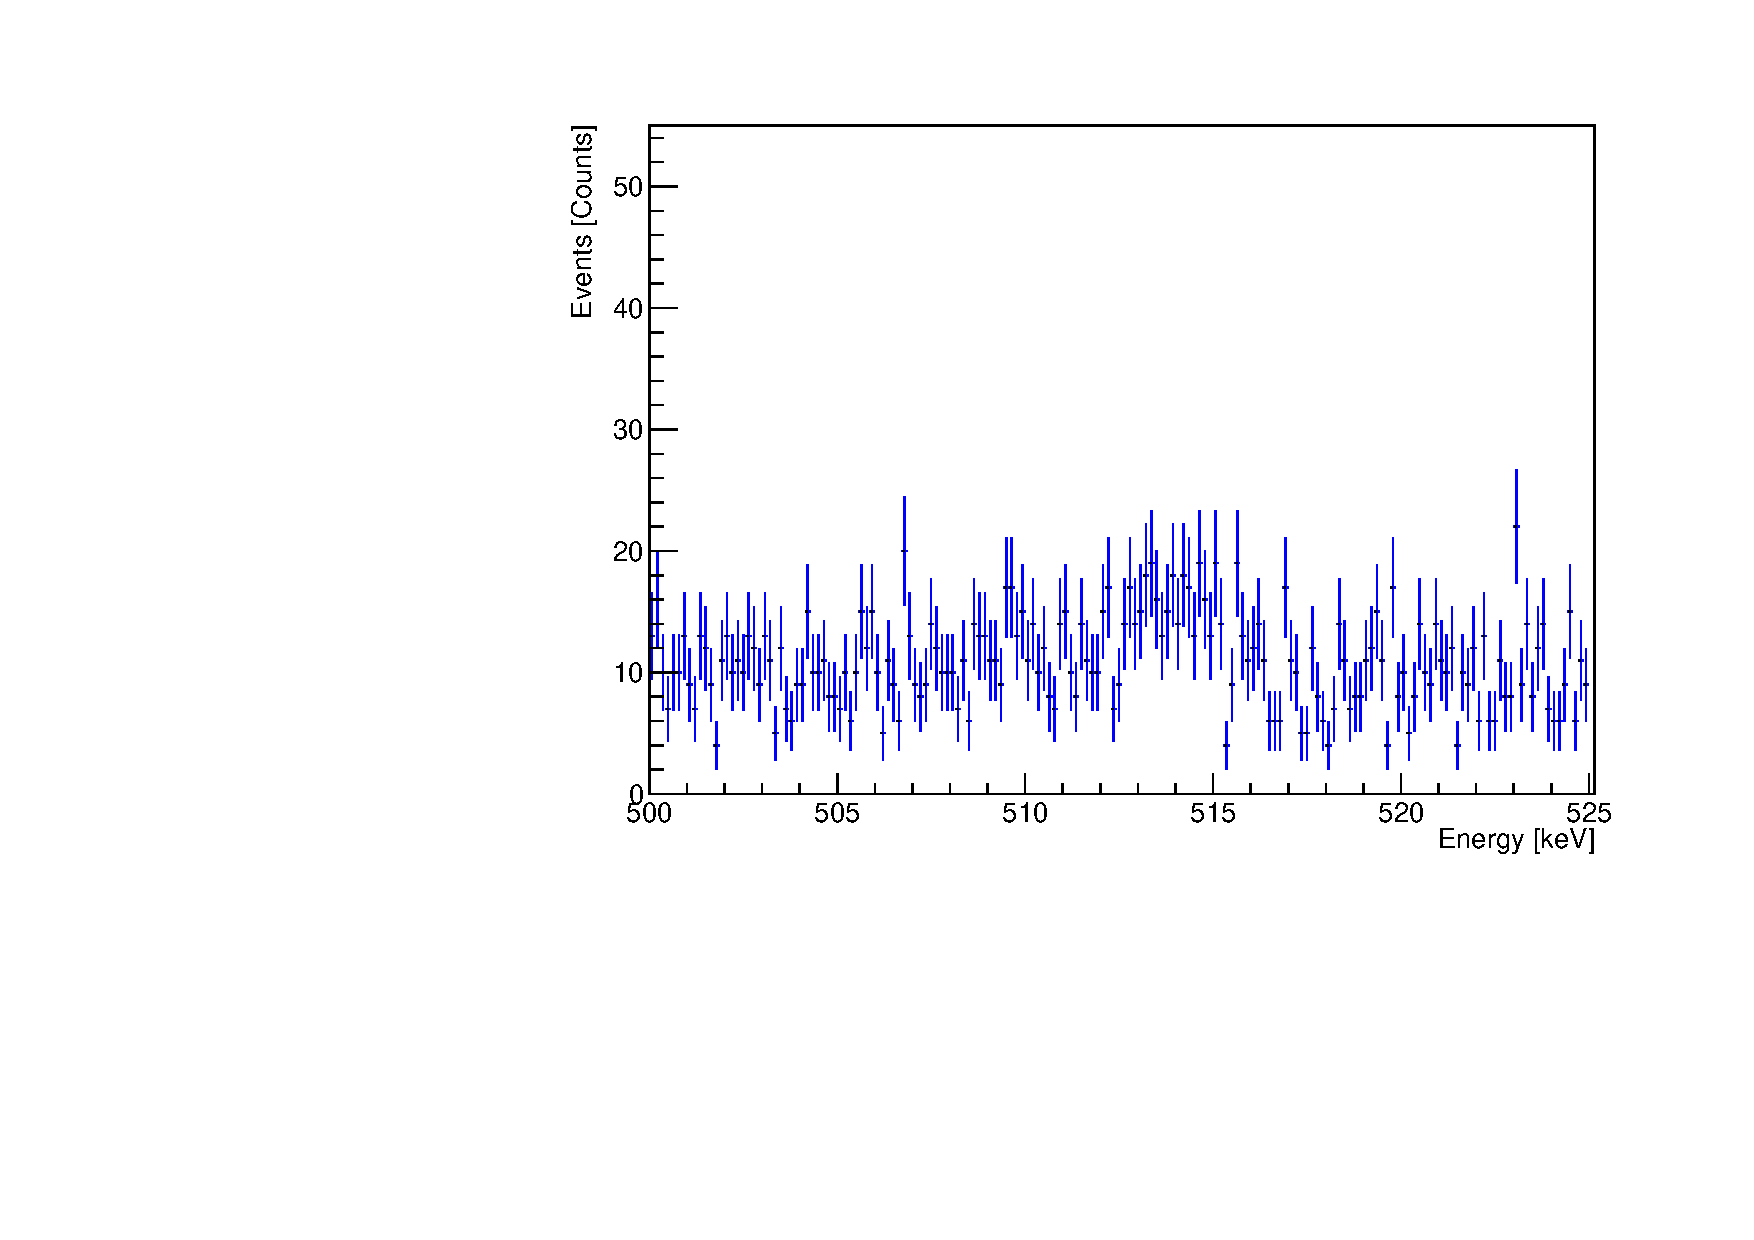
\includegraphics[width=75mm]{./Bilder/500525LArVetoCOAX.pdf}
  \caption{COAX}
  \label{fig:LArCOAX}
\end{subfigure}
    \caption{Energy spectra from 500 to 525 keV after standard \gerda\ analysis cuts and LAr veto.}
\end{figure}

\begin{figure}[t!]
	\centering
	\begin{subfigure}{.5\textwidth}
		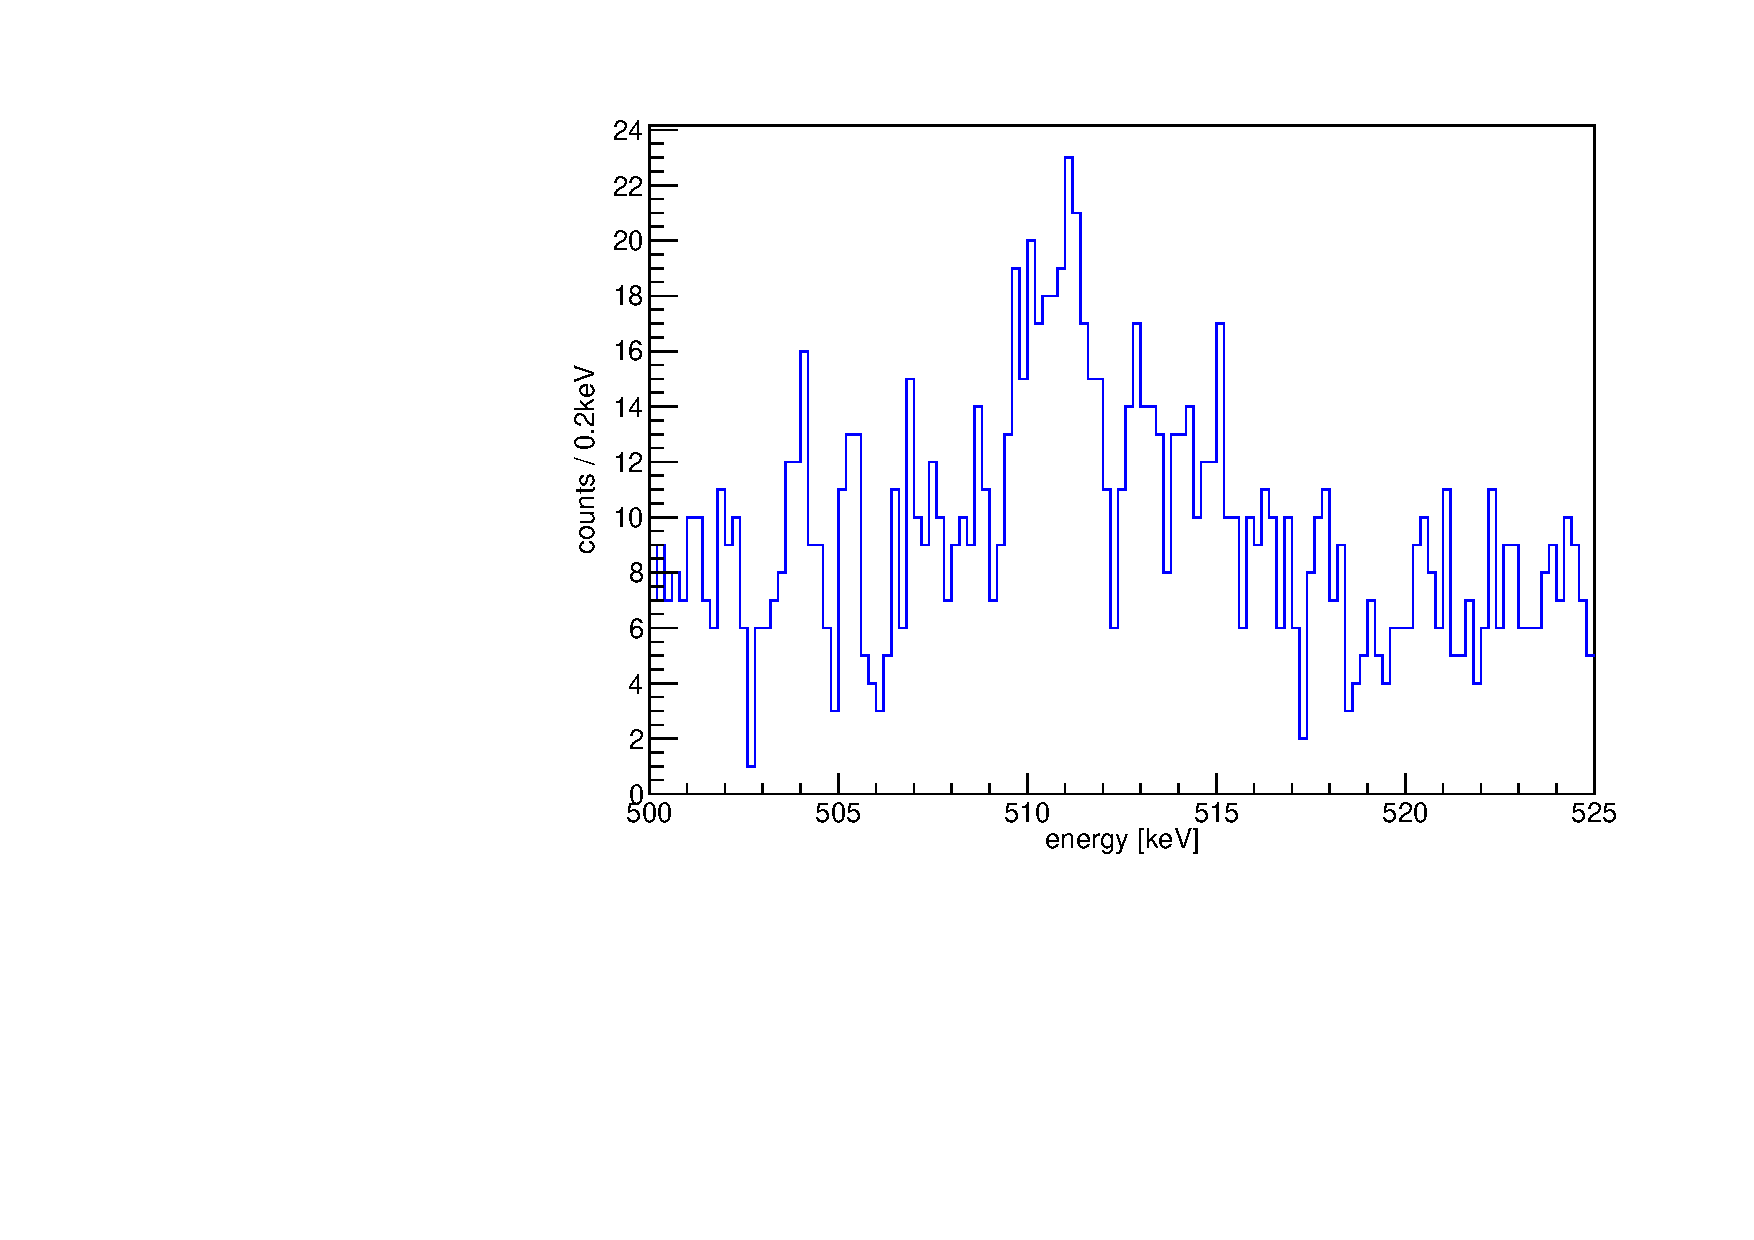
\includegraphics[width=75mm]{./Bilder/AntiLArBEGe.pdf}
		\caption{BEGes}
		\label{fig:AntiLArBEGes}
	\end{subfigure}\hfill%
	\begin{subfigure}{.5\textwidth}
		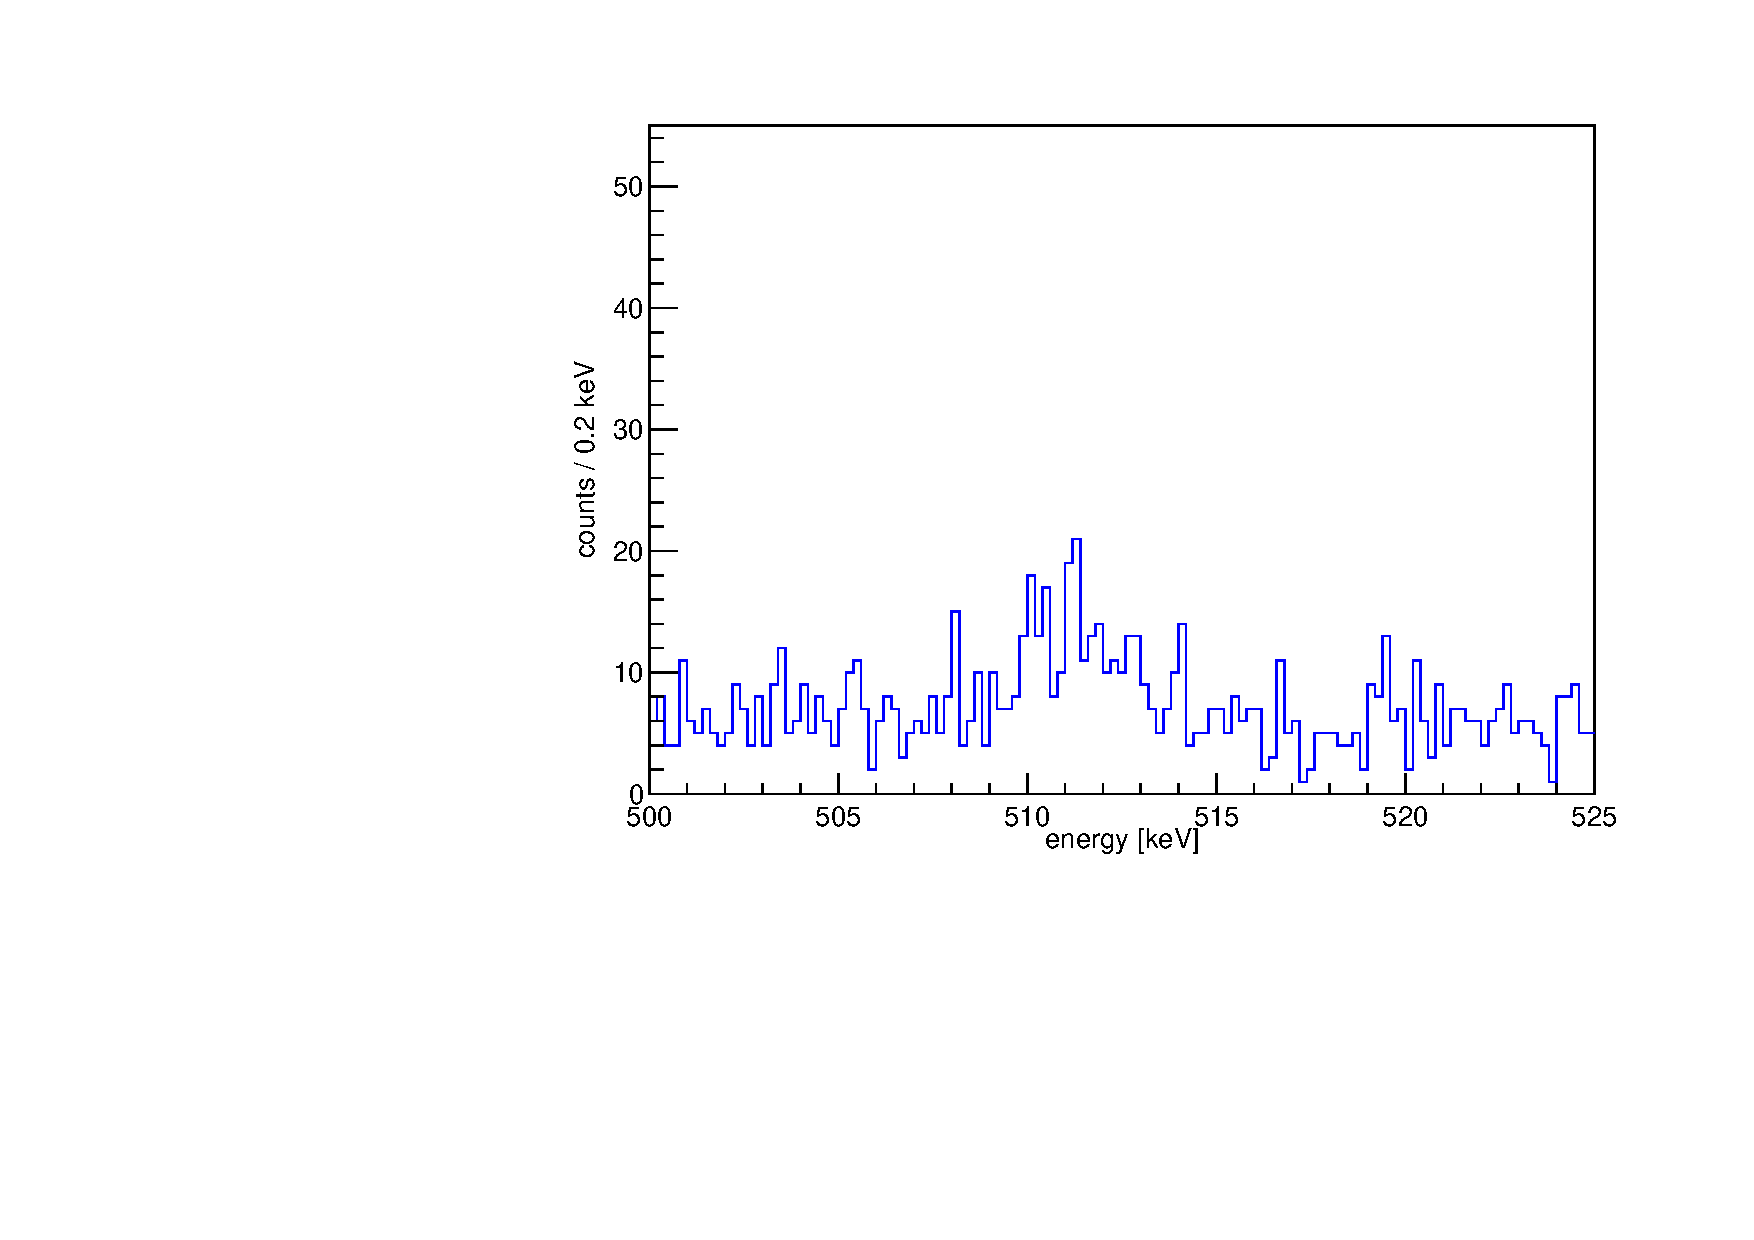
\includegraphics[width=75mm]{./Bilder/AntiLArCOAX.pdf}
		\caption{COAX}
		\label{fig:AntiLArCOAX}
	\end{subfigure}
	\\
	\vspace{0.5cm}
	\caption{Energy spectra from 500 to 525 keV }
\end{figure}

In order to have a better visualization which events have been rejected, all events that triggered the LAr veto are plotted in figures \ref{fig:AntiLArBEGes} and \ref{fig:AntiLArCOAX}).
From those you can see that the majority of the filtered events had an energy around the 511 keV mark.
\\

\section{Search for pre-coincidence}
\label{sec:precoince}

Because the line count would in this case be smaller than in the unfiltered case it is of interest to investigate whether some of the \Kr\ decay caused events might be possible to recover.
The absolute number of events filtered out by the LAr veto in the energy range of 509 to 519 keV is 1728.
This number is too big to look at every individual case manually.
\\

Luckily, the excited \nuc{Rb}{85m} state has a half life of 1.015 \(\unit{\mu s}\).
This means that one should be able to measure pre-coincedence events of the beta creating scintillation light before the germanium detector event.
This way one can hopefully identify the majority of events created by \Kr\ decays over the rest of the filtered signals.
For this purpose, the events used for the investigation must be limited to those that have a negative time difference between the germanium events and the photomultiplier signal.
The time difference for each individual liquid argon events is already analyzed and stored in the vector $"$triggerLAr$"$ of the Tier3 data set.
This vector has the same number of dimensions as photomultipliers and each entry is indexed with the corresponding input channel of one.
The entries of this vector are again vectors that store the time difference for each signal that triggered the LAr veto in the corresponding channel.
Since only the earliest trigger event of the photomultiplier is of interest for the analysis,  for reasons of simplicity only the first entry of this internal vector will be used as they are ordered in ascending order.
From this point, only events where at least one photomultiplier has measured a negative time difference are used for the recovery analysis.
\\

In addition, as already mentioned earlier, the energy of the released beta electron is very low.
This means that one can expect from a \Kr\ decay into an excited state of \nuc{Rb}{85m} that only a small number of photomultipliers should measure a signal.
This is because the effective scintillation yield of the \gerda\ setup is about 60 phe/MeV.
With a mean energy of 47.65keV one can expect that to measure 1 to 4 photons per decay.
thereforee, only events with a maximum of four different triggered photomultipliers are used in the further analysis.
This amount of coincedently triggered photomultiplier leaves still a lot of events.
But due to the fact that later in the analysis a manually investigation into the individually measured events will be performed the filter can be a little coarser here.
\\

\begin{figure}[t!]
	\centering
	\ifmakefigures%
	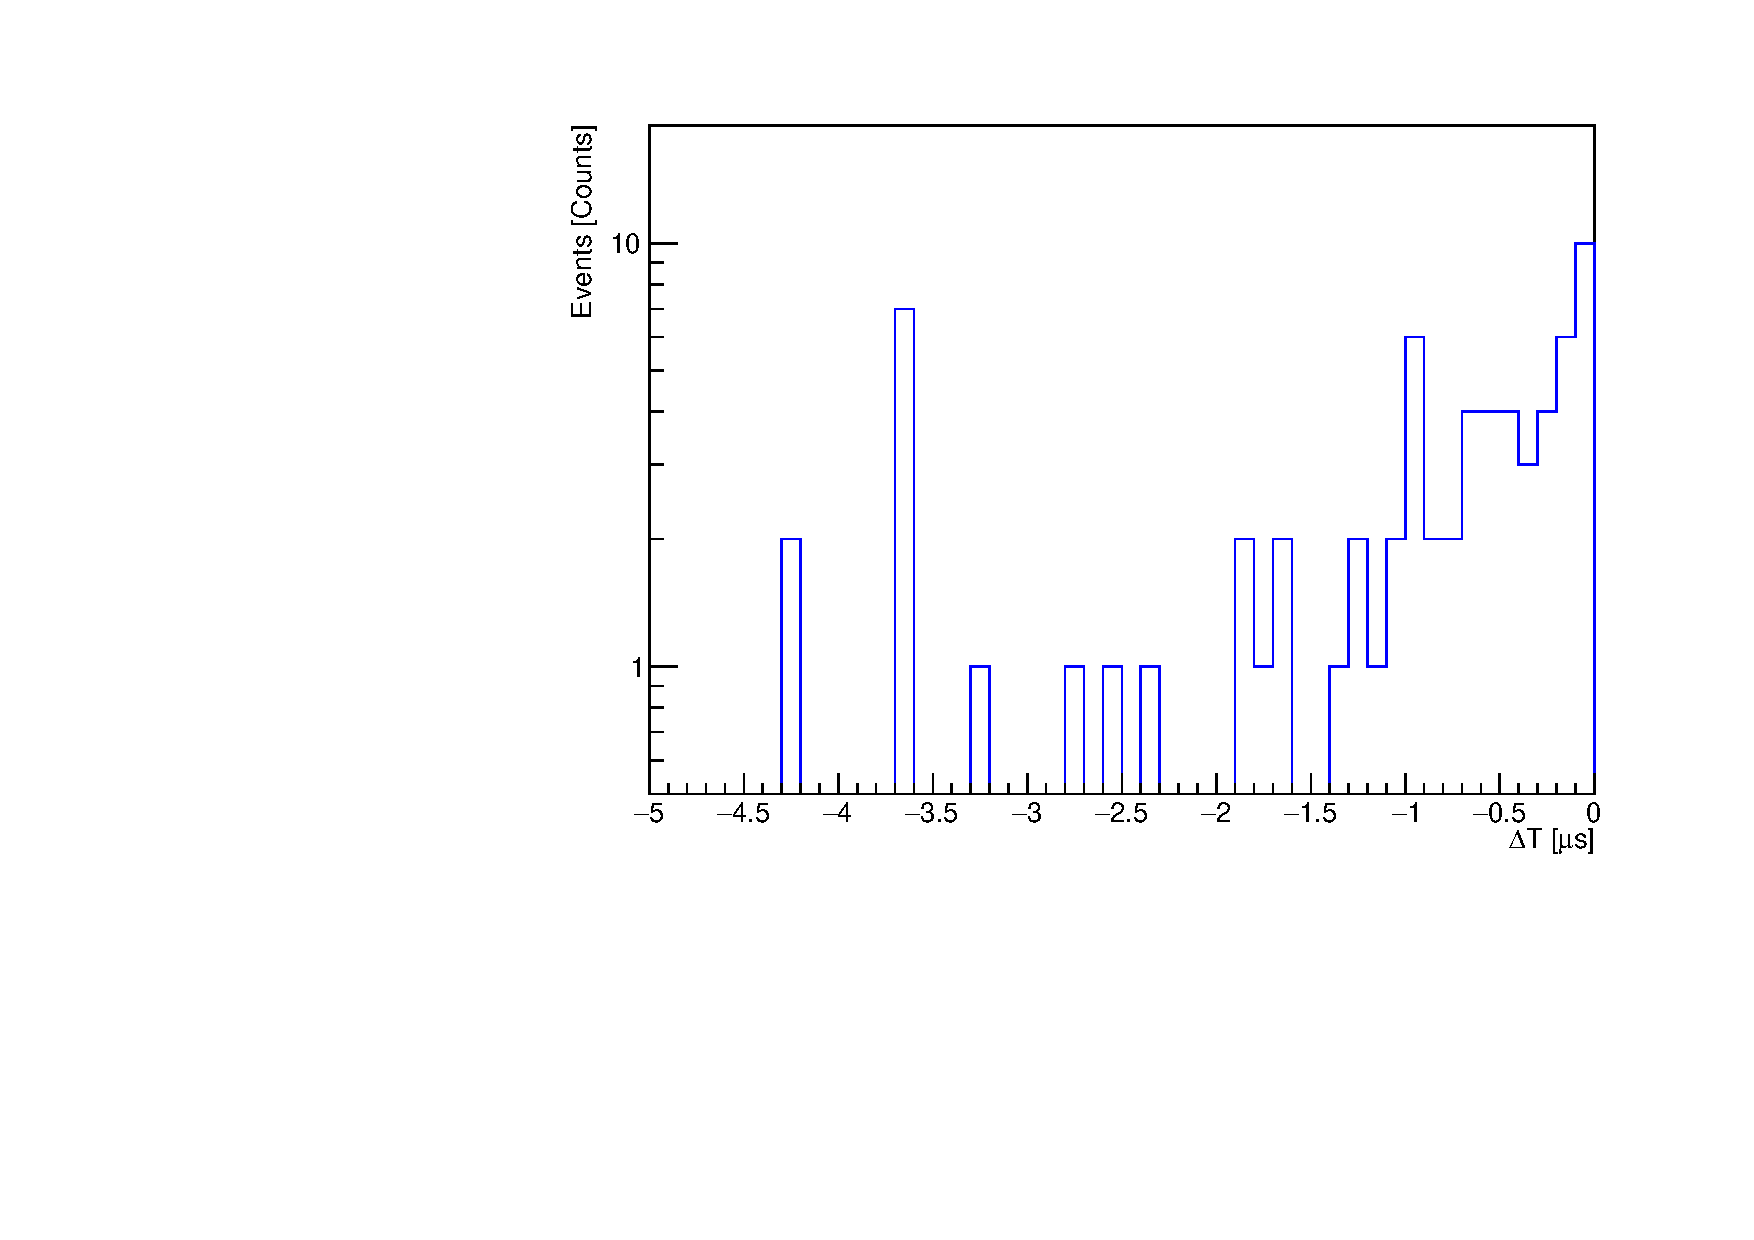
\includegraphics[width=100mm]{./Bilder/TriggerTimeOnly4.pdf}
	\fi%
	\caption{
	    Counts plotted over the time difference between the germanium detector event and the signal in the photomultipliers.
	    The range of the plot only shows the negative time difference from -5 to 0 $\mu$s.
	    This means that all events creating this plot measured a photomultiplier signal before an germanium detector signal.
	    Due to \nuc{Rb}{85m}'s half life of 1.015$\mu$s an exponential increase should be identifiable but with the low amount of counts no statement can be made. 
	}
    	\label{fig:Trigger4}
\end{figure}

Applying these two restrictions to the LAr veto filtered events and using from those only those photomultiplier events with a signal strength of at least 0.5 phe results in a distribution as shown in figure \ref{fig:Trigger4}.
Only the signals that have measured at least 0.5 phe are of interest because they had the necessary intensity to trigger the LAr veto. 
The x axis is the time difference of the events in the photomultipliers from the signal measured in one of the Germanium detectors.
Theoretically it should be possible to see a exponential increase from the negative scale towards a vanishing time difference.
But due to the small number of events, it is basically impossible to make any statements about the course of these events.
\\

Nevertheless, the number of events of interest was reduced from 1728 to only 55.  
These remaining events can now be manually examined with a software called GerLa.
This tool allows one to search for a specific events and see all recorded signals of the Germanium detectors and the photomultipliers around the time frame of this event.
\\

With this program one can now perform a manual filter.
This can be done by looking at the remaining 55 events individually and decide whether to reject an event or not using a specific protocol.
This protocol consists of rejecting every event that has a combined light intensity of over 5 phe and every event that only has a negative time difference in a signal weaker than 0.5 phe.
The upper limit of the light intensity originates again from the expected number of photons as described earlier.
\\

\begin{figure}[t!]
	\centering
	\ifmakefigures%
	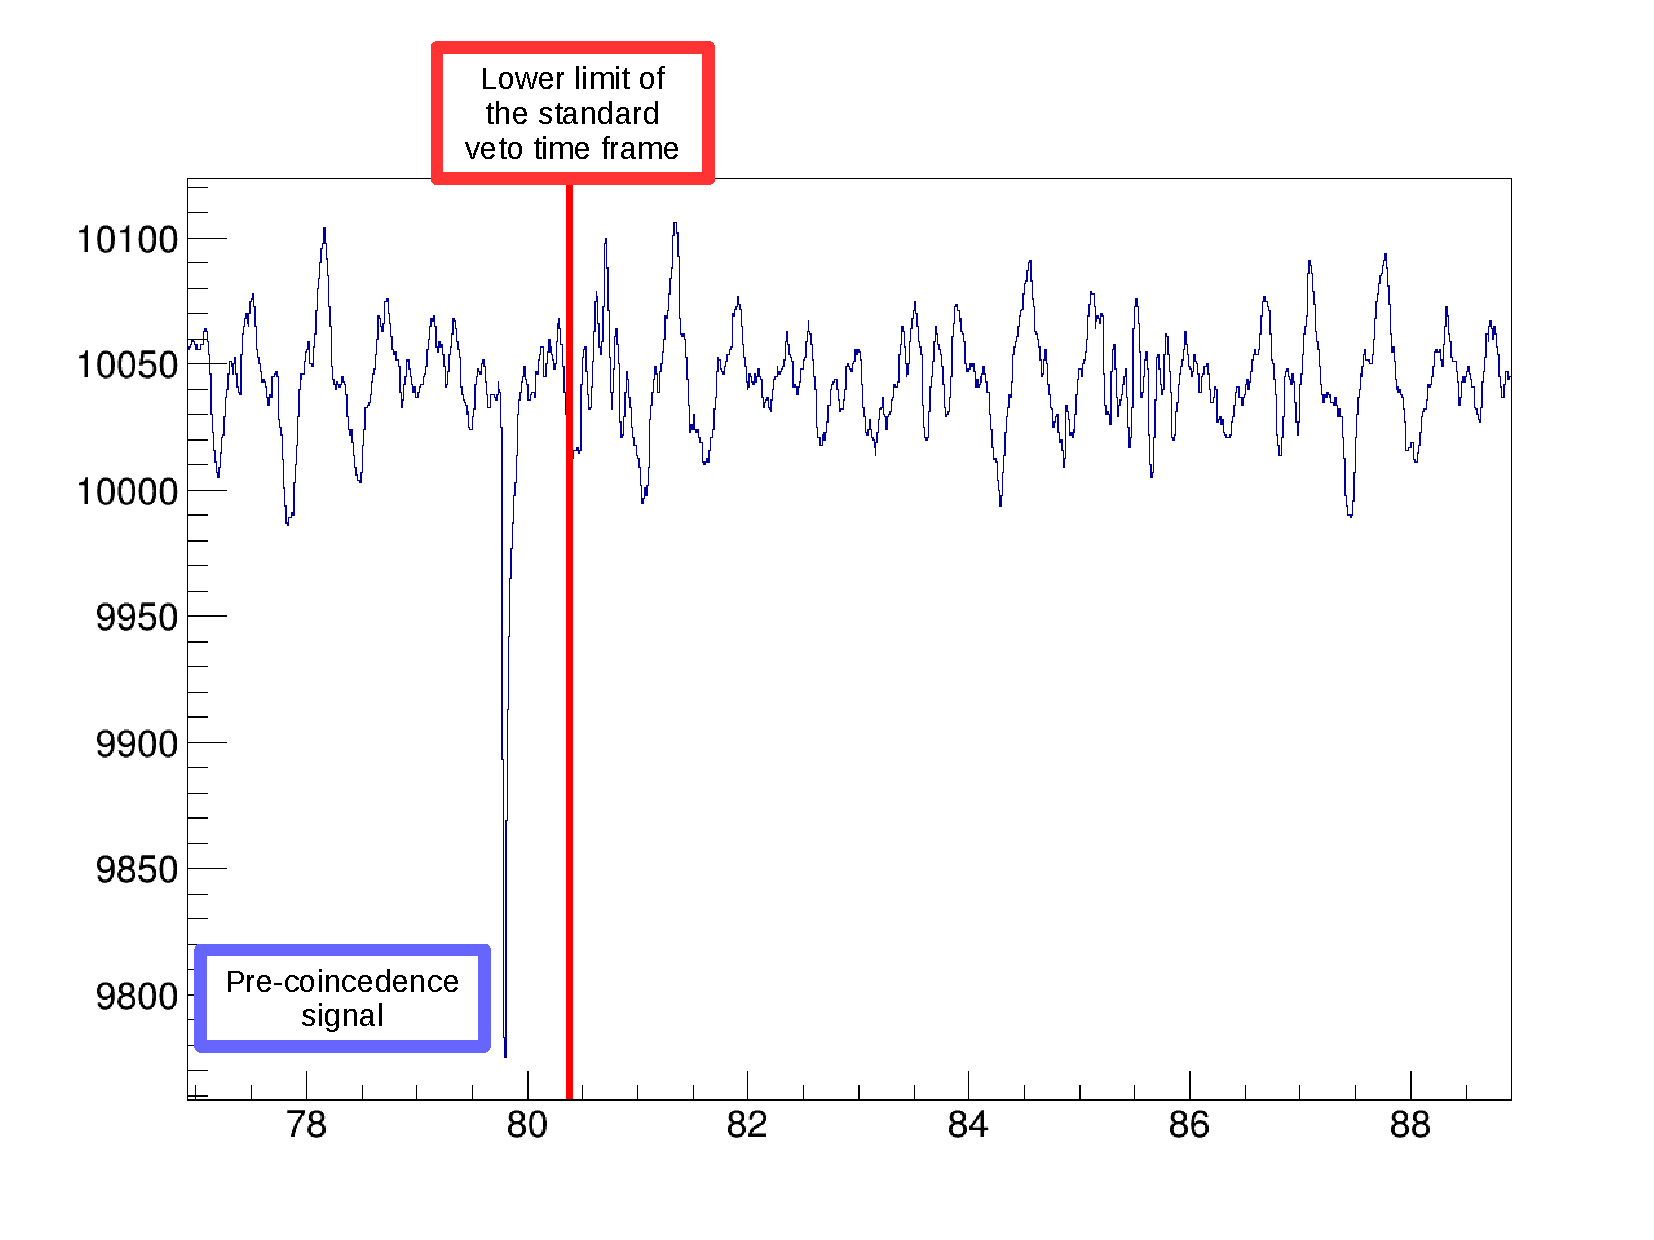
\includegraphics[width=100mm]{./Bilder/BeispielSignal.pdf}
	\fi%

	\caption{
    The recorded signal of photomultiplier tube P4 in event 1614036. 
    In it is the raw energy signal plotted over the recorded time frame. 
    The blue line indicates the moment in time in which an event in one of the germanium detectors was measured. 
    From it one can see that the photomultiplier signal occurred before the germanium detector signal.   
    }
    	\label{fig:BeispielSignal}
\end{figure}

While going through each of the 55 events, it quickly was realized that this procedure does not work as well as we hoped it would.
From the remaining 55 only a handful of events were unambiguous enough that one can claim that the photons must originate from expected beta electron.
After this much filtering it can assume the few that were found are probably all in fact caused by a \Kr\ decays.
Signals like the one shown in figure \ref{fig:BeispielSignal} are a rare example of an almost model signal that were expected to be measured.
The great majority of other events were either background events in the SiPM that seem to randomly triggered the LAr veto or the combined signal strength was much higher than 5 phe.\\

This leads to the conclusion that the majority of signals in the photomultiplier with a negative time difference were in fact not caused by the beta electrons scintillation light but rather coincidences with other signals.
This means it is practically impossible to recover any of them with the process presented here.

The recovery attempt has failed.
\\

Nevertheless we are still able to make some qualitative estimations about why approach might not have worked. 
The problem of this recovery attempt seems to be that the majority of events detected with a negative time difference are in fact background events.
This conclusion came from the fact that almost none of the events investigated have shown the features we expected from them.

An indicator for this can be seen in the fact that the majority of light signals have been measured in the PMTs.
As it will be shown in section \ref{sec:MonteCarlo514}, basically all of the decays that created a measurable 514keV event have happened in the vicinity of the detectors.
The detectors themselves should already block some of the light but when a photon is detected in a photomultiplier it would most likely be a SiPM.
This is because the nylon fibers surrounding the germanium detectors are more likely to absorb and guide the scintillation light to the SiPM than a photon to reach a PMT above or below the detector arrays.
Now that the majority of the detected light events are measured in the PMTs it is very unlikely that these are caused by a \Kr\ decay.

%That the majority of the 
%This might also be able to be seen from figure \ref{fig:AntiLArBEGes} and \ref{fig:AntiLArCOAX}.
%From them one was able to see that the LAr veto also filtered out some of the 514keV line events.
%But from it can also be seen, that the ratio of events filtered out at the 514keV mark over the non filtered value [$N_{\unit{vetoed}}(514\unit{keV})/N_{\unit{unfilered}}(514\unit{keV})]$ is of about the same size as in the background area whereas the positron electron peak shows much higher ratio.
%Considering this the peaks in \ref{fig:AntiLArBEGes} and \ref{fig:AntiLArCOAX} probably came to be  due to the same relative amount of events have their liquid argon veto triggered because of background events.
Because of this it is rather questionable whether the LAr veto is even a good identifier to use when it also filters out events in which background can trigger the veto.
A satisfactory answer however will only be able to obtain through a quantitative analysis which will be performed in the following chapter.
\\

\section{Fitting}
\label{sec:Fitting}

The spectra from before and after the LAr veto will now be fitted.
From the determined fit parameters the amount of measured \Kr\ decay events can then be calculated by integrating over the isolated Gauss function.
\\

The spectra before the LAr vetoes \ref{fig:NoFilterBEGes} and \ref{fig:NoFilterCOAX} show two peaks.
This requires the fit function to include two Gaussian functions from which only the parameters of the second peak will then be used for further analysis.
Additionally to the two Gaussian peaks, a constant background parameter will be added.
Theoretically, the \nuc{Ge}{76} spectrum creating the background changes with energy.
In the investigated area, however, its overall change is so small, as seen in all previously plotted spectra, that it can be approximated as constant. 
\iffalse
When looking at the not LAr veto filtered spectra we can see that over the course of the displayed energy interval no real change of the background can be seen (see figure \ref{fig:NoFilterBEGes} and \ref{fig:NoFilterCOAX}).
Theoretically however, one can expect the background count rate to behave like the phase-space function of the dominant \nuc{Ge}{76} and therefore change with energy.
So it is necessary to also consider this change in count rate over energy in the fit function.
The phase-space function of \nuc{Ge}{76} is very complex.
In this case however the energy interval is relatively small compared to the complete spectrum.
This allows the approximation that its phase-space function changes like an exponential decrease.
\fi
The resulting fit function is shown in equation \ref{equ:FitNoFilters}.
\\

\begin{equation}
\mathrm{f}(x) = \mathrm{A}\frac{1}{\sqrt{2\pi}\mathrm{C}}\exp\left(-\frac{(x-\mathrm{B})^2}{2\mathrm{C}^2}\right) + \mathrm{D}\frac{1}{\sqrt{2\pi}\mathrm{C}}\exp\left(-\frac{(x-\mathrm{E})^2}{2\mathrm{C}^2}\right) + \mathrm{G}
\label{equ:FitNoFilters}
\end{equation}
\\

In figure \ref{fig:FitNoFilterBEGes} and \ref{fig:FitNoFilterCOAX} are the resulting fit plots displayed.
The concrete fit parameter values can be seen in the table of the figures.
Fitting parameters B and E - the mean values of the peaks - where fixed to the values of 511 keV and 514 keV respectively.
All other values were left free under the condition of a positive value.
Also, Parameters C - the sigma value - was used in both peaks as the resolution of the detectors should not vary much over this small interval.
Their measured values resemble the expected value of ... and ... calculated from the respective resolution relatively well.  
\\

\begin{figure}[t!]
	\centering
	\begin{subfigure}{.5\textwidth}
		\centering
		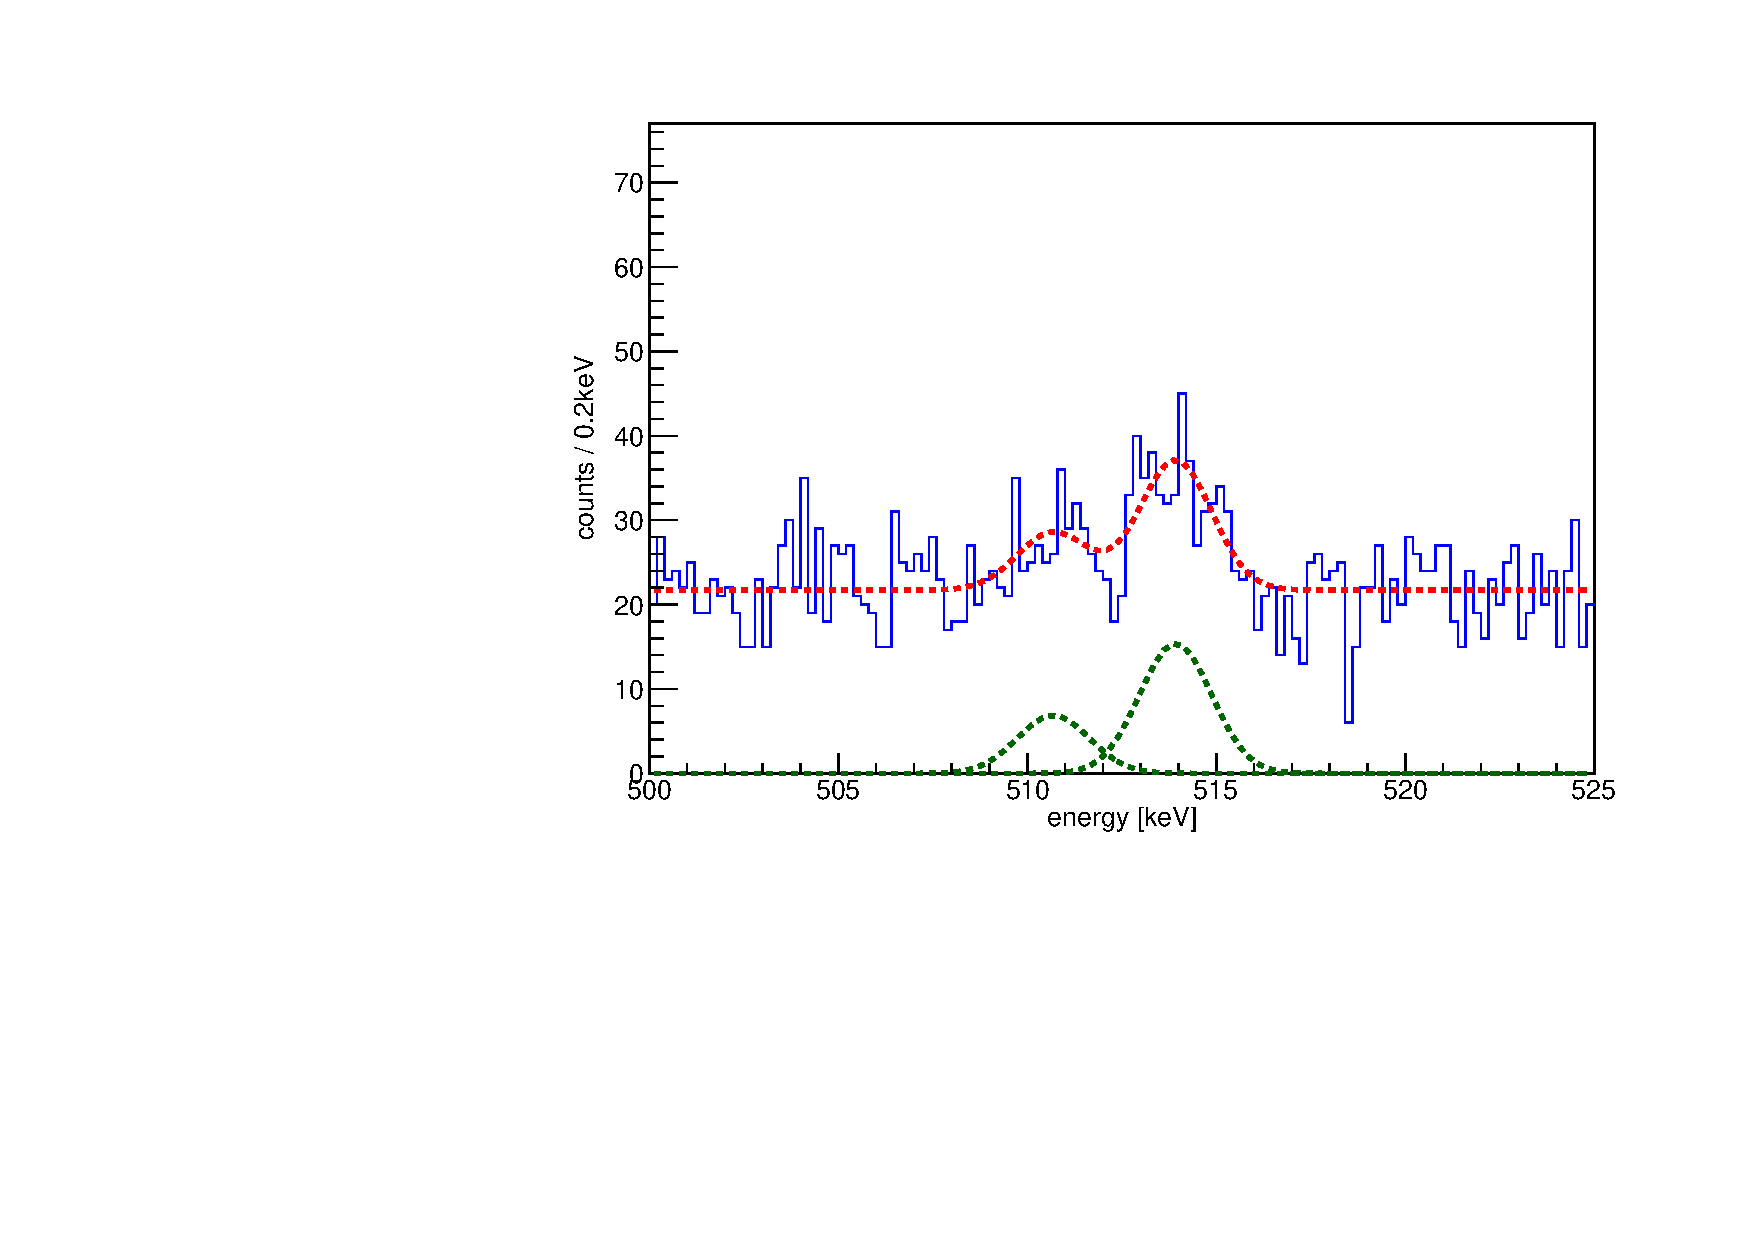
\includegraphics[width=75mm]{./Bilder/500525FitNoFilterBEGes.pdf}
		\caption{BEGes}
		\label{fig:FitNoFilterBEGes}
	\end{subfigure}\hfill%
	\begin{subfigure}{.5\textwidth}
		\centering
		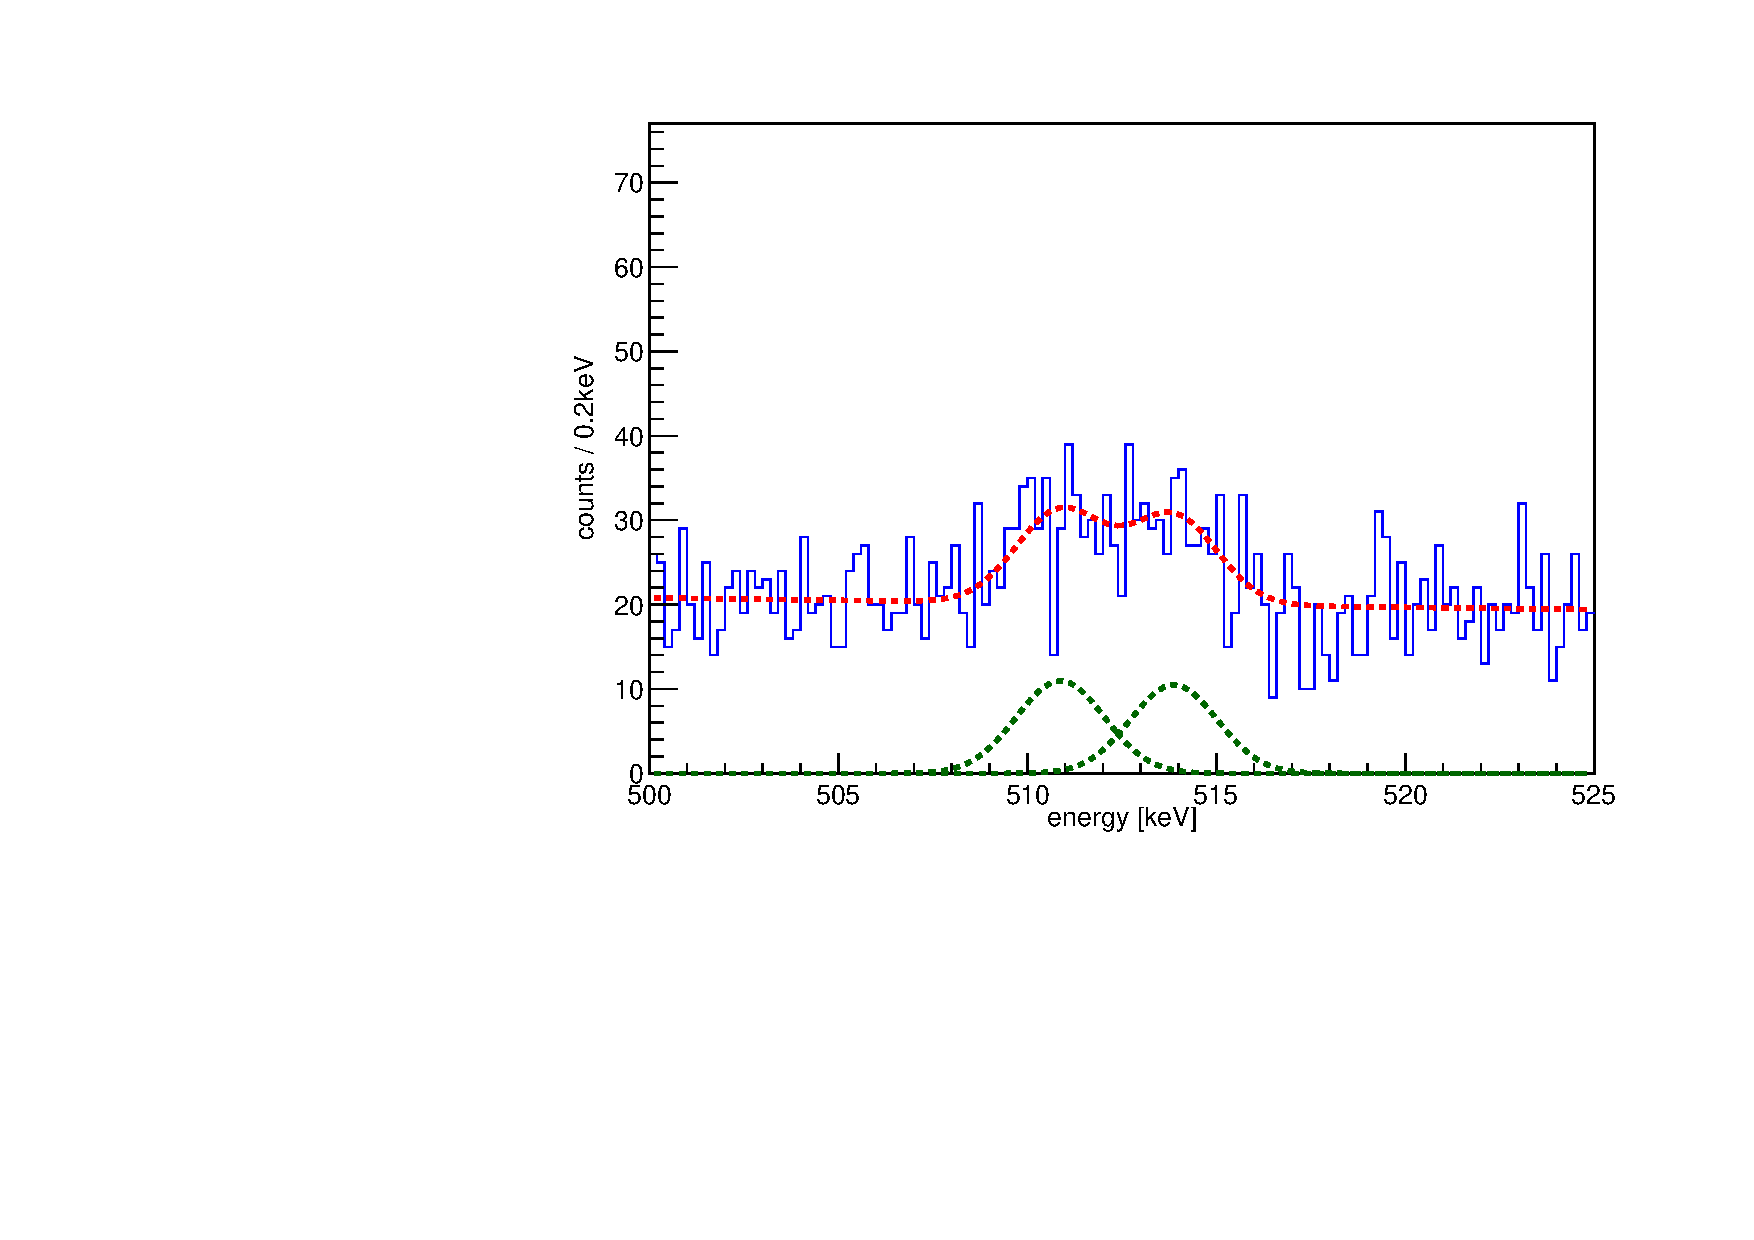
\includegraphics[width=75mm]{./Bilder/500525FitNoFilterCOAX.pdf}
		\caption{COAX}
		\label{fig:FitNoFilterCOAX}
	\end{subfigure}
    \\
	\caption{
		Fitted energy spectra from 500 to 525 keV before the LAr veto cut. 
		Function \ref{equ:FitNoFilters} was used as fit function. 
		Its course is indicated in red. 
		The two green plots at the bottom of the figures indicate the two independent peak responsible for the deviations. 
		}
\end{figure}
\\

\iffalse

\begin{table}[t!]
\centering
\begin{tabular}{|l|c|c|}
\hline
Name	& Value [BEGe] & Values [COAX]\\ 
\hline
A [counts $\times$ / 0.2 ] &	(15.98 \(\pm\)	4.54)&	(31.93\(\pm\)7.08)	\\	
\hline
B [keV] &	(510.87 \(\pm\)	0.22)&	(510.88 \(\pm\)	0.190)\\	
\hline
C [keV] &	(0.952 \(\pm\)	0.011)	&	(1.165 \(\pm\)	0.010)	\\
\hline
D [counts / 0.2 keV] &	(36.66 \(\pm\)	4.99)	&	(30.40 \(\pm\)	5.24)	\\
\hline
E [keV] &	(513.95 \(\pm\)	0.16)	&	(513.87 \(\pm\)	0.14)	\\
\hline
F [keV] &	(0.953 \(\pm\)	0.014)	&	(1.145 \(\pm\)	0.012)	\\
\hline
G [counts / 0.2 keV] &	(11.98 \(\pm\)	5.27)	&	(11.35 \(\pm\)	7.45)	\\
\hline
H [counts / 0.2 keV] &	(189.92 \(\pm\)	110.05)	&	(996.72 \(\pm\)	972.62)	\\
\hline
I [1/keV] &	(5.80 \(\pm\) 1.22)$\times10^{-3}$	&	(9.24 \(\pm\)1.83)$\times10^{-3}$ \\
\hline

\end{tabular}
\caption{
	Fit parameters of fit function \ref{equ:FitNoFilters} applied on the spectra of the respective detectors. 
	Variable A and D correspond to the amplitudes of the two Gaussian peaks, B and E to the position of their maxima, C and F their standard deviation. 
	On the other hand is G the constant background, H the amplitude of the exponential background and I its decrease parameter.
	}
\label{tab:FitParNoFilter}
\end{table}
\\
\fi

However, the only fit parameter that is of real interest here is variable D.
Its value is the amplitude of the second Gaussian peak.
Because the Gaussian peak was already chosen in the normalized form this value also represents the amount of \Kr\ decays measured per binning of the histogram.
From it one can finally determine an amount of $N_{\mathrm{peak,BEGe}} = (183\pm25)$ counts in the peak of the BEGe spectrum and $N_{\mathrm{peak,COAX}} = (152\pm26.2)$ counts in the COAX spectrum.
\\

Now to spectrum after the LAr veto.
Fit function \ref{equ:FitNoFilters} will also be used.
This is an advantage because it will also fit around a possible remaining 511 keV peak that might otherwise would have affected the outcome.

\iffalse
As mentioned above one can assumed that the positron electron annihilation peak is fully suppressed.
therefore only one Gaussian peak has to be fitted together with the background function.
Additionally in the ideal case, that the majority of all \Kr\ decay events got through the LAr veto, one can expect the amplitude of the Gaussian peak to be equal to the amplitude of the not LAr veto filtered case.
The fit results in the function displayed in equation \ref{equ:FitFilters}.
\\ 

\begin{equation}
\mathrm{f}(x) = \mathrm{A}\frac{1}{\sqrt{2\pi}\mathrm{C}}\exp\left(-\frac{(x-\mathrm{B})^2}{2\mathrm{C}^2}\right) + \mathrm{D}\exp\left(\mathrm{-E}x\right) + \mathrm{F}
\label{equ:FitFilters}
\end{equation}
\\
\fi

Diagrams \ref{fig:FitLArVetoBEGes} and \ref{fig:FitLArVetoCOAX} show the fitted plots.
As above, the amplitude D of the second Gaussian peak corresponds to the number of events measured in the area of the peak per binning.
This results in an amount of $(120\pm19.3)$ counts for the BEGe and $(128\pm22.1)$ for the COAX spectrum.
\\

Compared to the values of the not filtered spectra however, it can be seen that the number of counts in the BEGe and in the COAX detectors have dropped considerably.
This means that some of the  \Kr\ decay events must have also been rejected by the LAr veto and a recovery would be necessary. !!!!! hier noch umschreiben !!!!!
But due to that not being possible those results can not be used in further course of this analysis.
The second approach was only intended as a cross-check for the values not filtered by LAr veto anyway, so no real loss there.
It still would have been great if it had worked as a crosscheck.
\\

\begin{figure}[t!]
	\centering
	\begin{subfigure}{.5\textwidth}
		\centering
		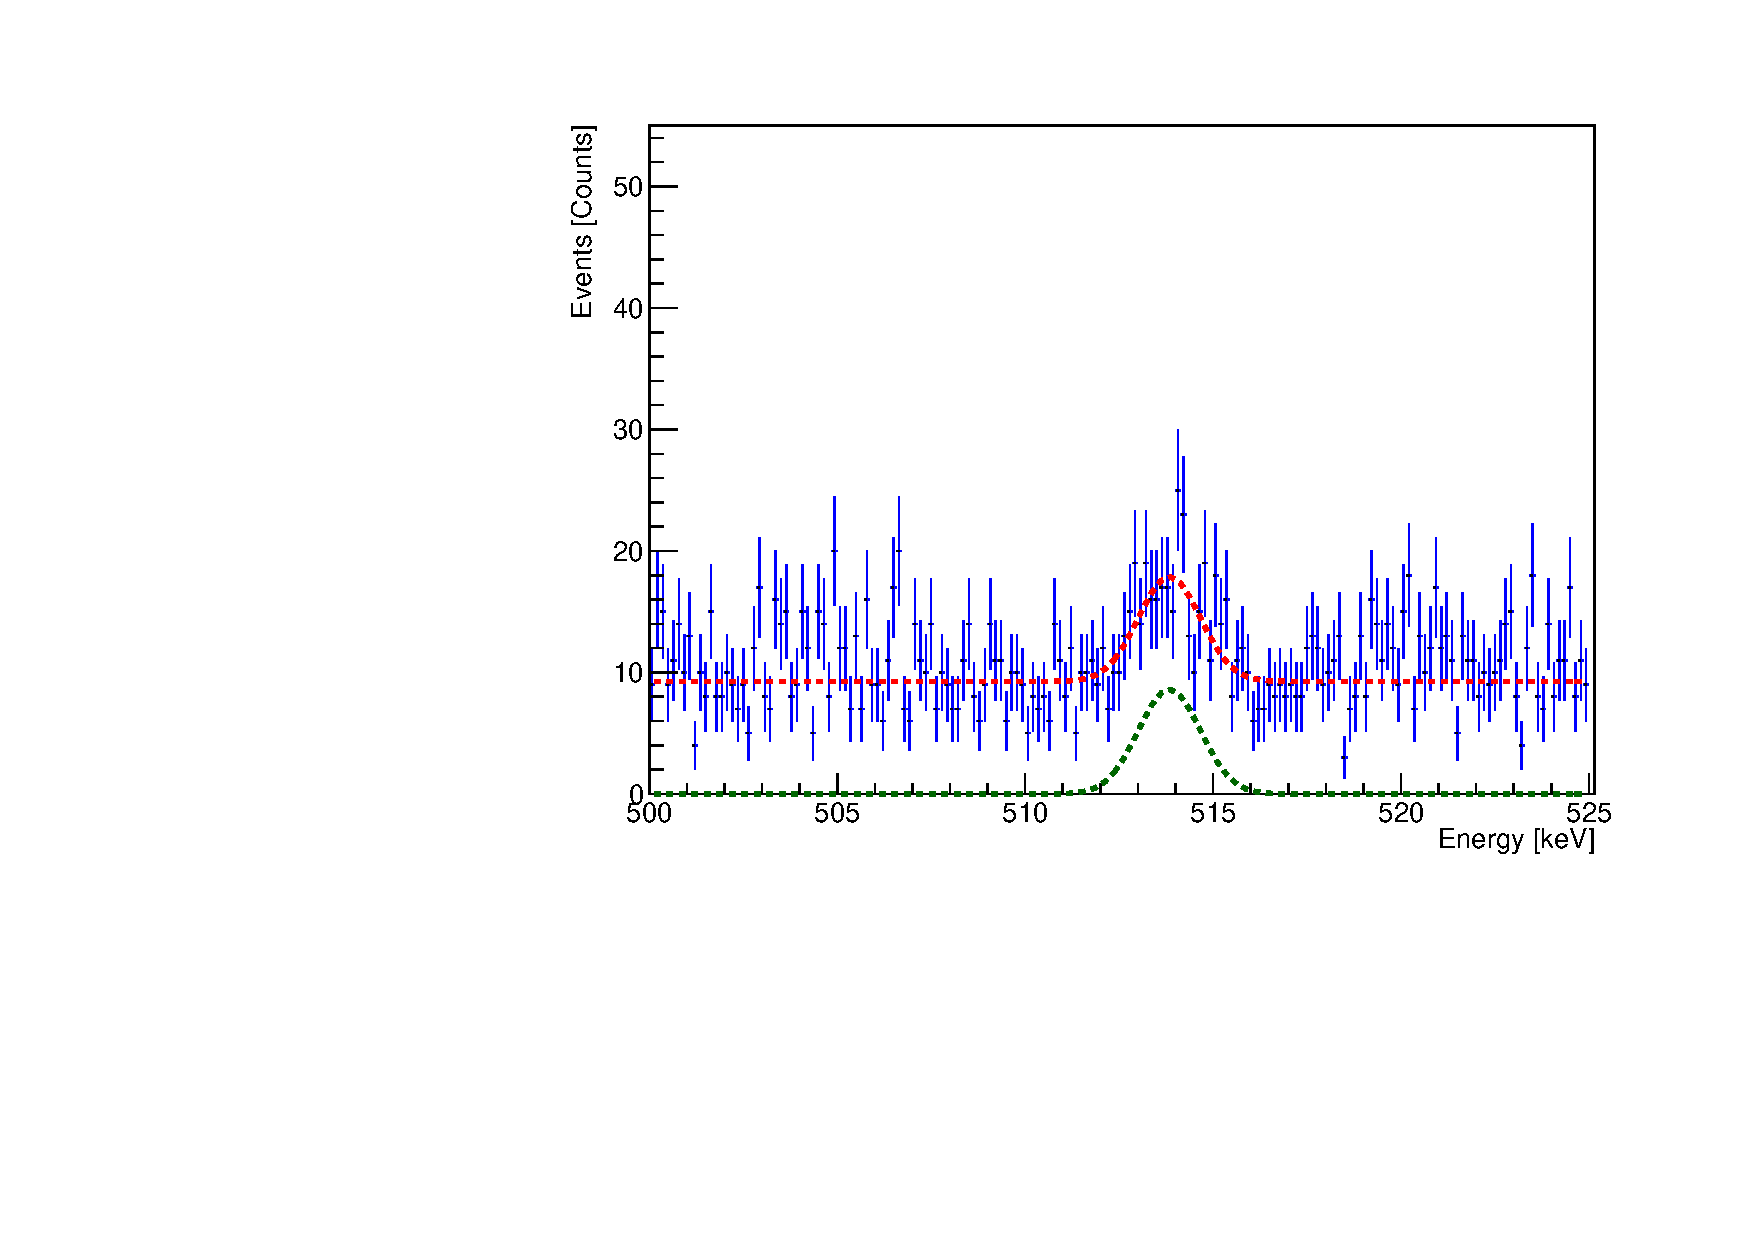
\includegraphics[width=75mm]{./Bilder/500525FitLArVetoBEGes.pdf}
		\caption{BEGes}
		\label{fig:FitLArVetoBEGes}
	\end{subfigure}\hfill%
	\begin{subfigure}{.5\textwidth}
		\centering
		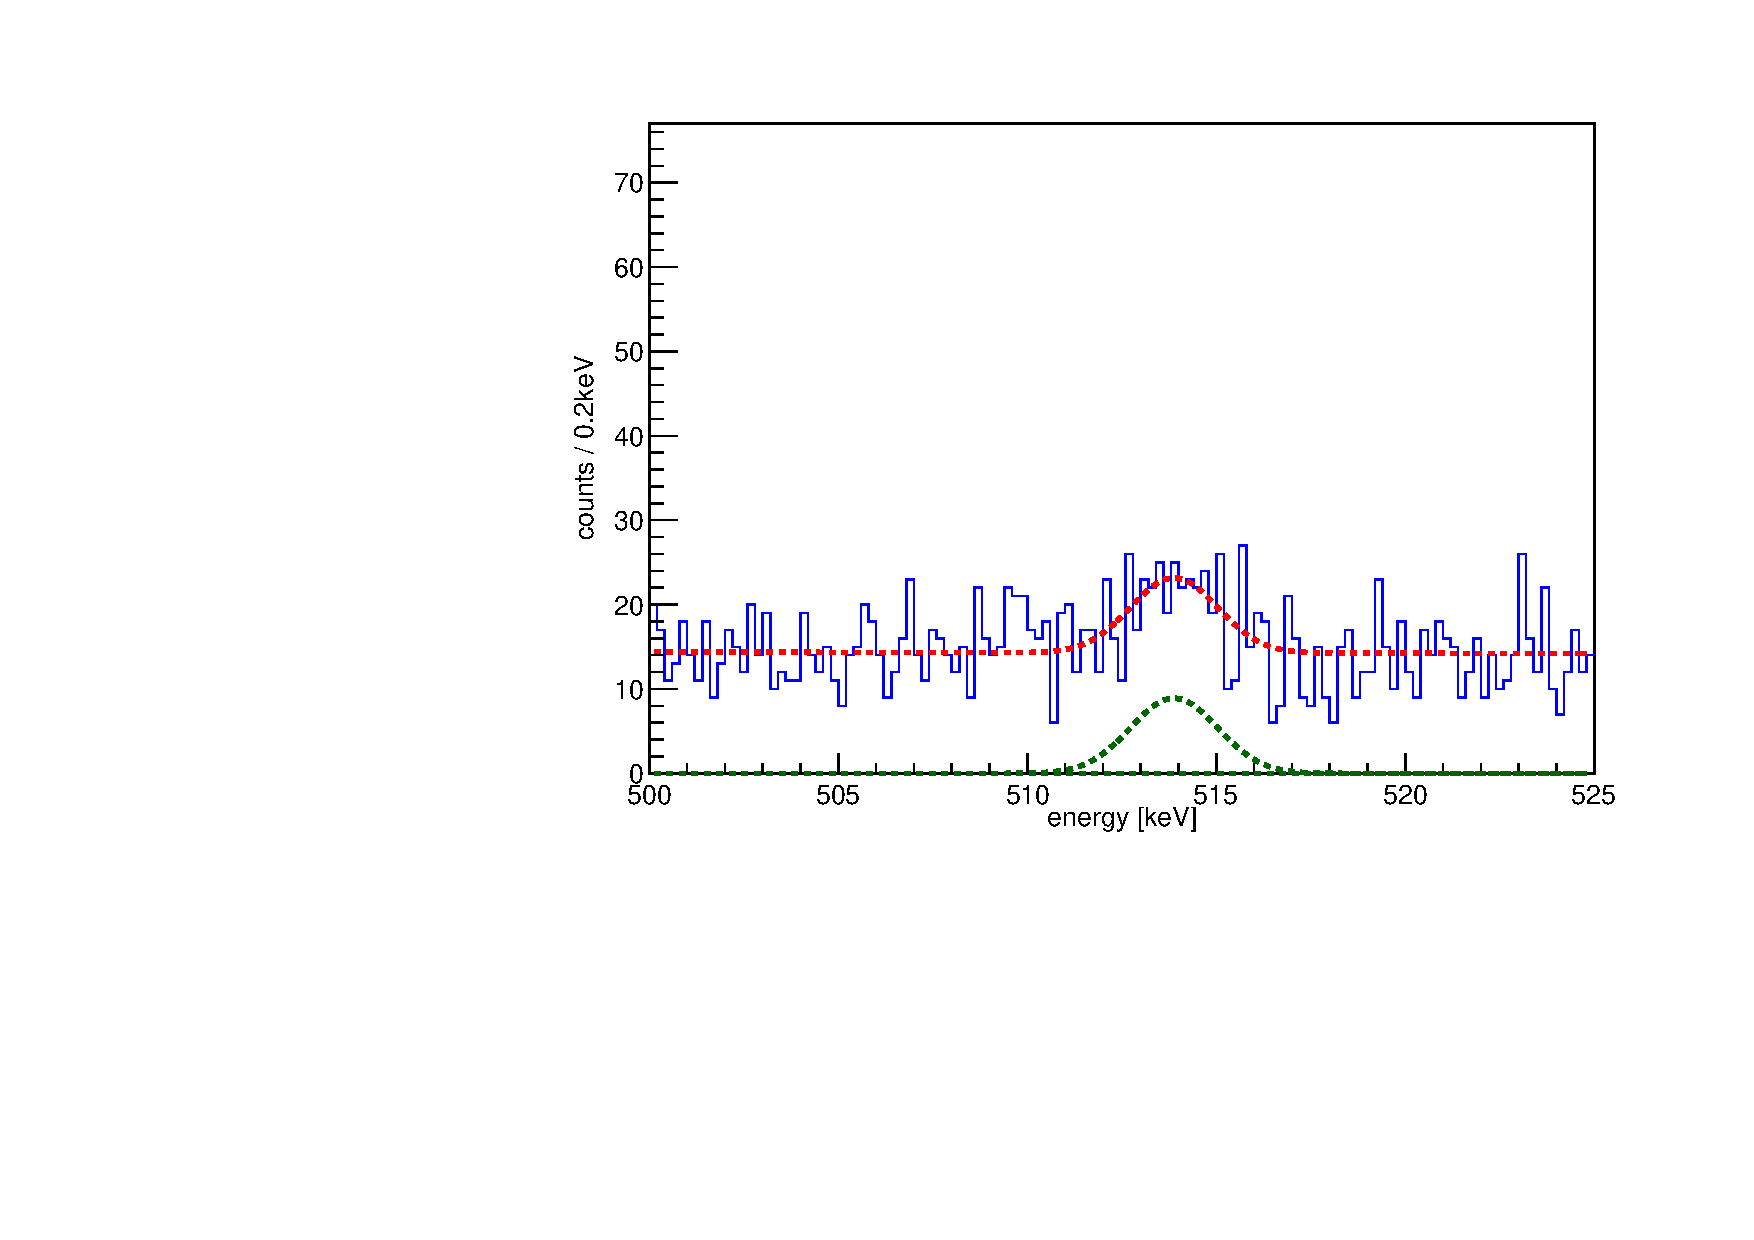
\includegraphics[width=75mm]{./Bilder/500525FitLArVetoCOAX.pdf}
		\caption{COAX}
		\label{fig:FitLArVetoCOAX}
	\end{subfigure}
	\caption{
	Fitted energy spectra from 500 to 525 keV when only considering those event that got though the Muon veto, the detector anti-coincidence veto and the LAr veto. 
	Function \ref{equ:FitFilters} was used as fit function. 
	Its course is indicated in red. 
	The green plots at the bottom of the figures indicate the peaks responsible for the deviation. 
	Their course was determined from the corresponding fit parameter.
	}
\end{figure}
\iffalse
\begin{table}[t!]
	\centering
	\begin{tabular}{|l|c|c|}
		\hline
		Name	& Value [BEGes] & Value [COAX]\\ 
		\hline
		A [counts  / 0.2 ] &	(24.094734$\pm$3.856334)&	(25.680418$\pm$4.424006)\\	
		\hline
		B [keV] &	(513.925781$\pm$0.129591)&	(513.884766$\pm$0.185506)\\	
		\hline
		C [keV] &	(0.952731$\pm$0.019180)	&	(1.145909$\pm$0.018075)\\
		\hline
		D [counts / 0.2 keV] &	(14.548210$\pm$0.349083)	&	(10.602730$\pm$8.090884)\\
		\hline
		E [counts / 0.2 keV] &	(0.607414$\pm$5.193491)	&	(10.000000$\pm$9.831094)\\
		\hline	
		F [1 / keV] &	(0.901209$\pm$2.409593)	&	(0.001950$\pm$0.004637)\\
		\hline
	\end{tabular}
	\caption{
		Fit parameters of fit function \ref{equ:FitNoFilters} applied on the spectra of the respective detectors. 
		Variable A correspond to the amplitudes of the Gaussian peak, B to the position of its maximum, C its standard deviation. 
		On the other hand is D the constant background, E the amplitude of the exponential background and F its decrease parameter.
		}
			\label{tab:FitParFilter}

\end{table}
\fi
\iffalse
Nevertheless, the line count rate $N_{\mathrm{peak,BEGe}}$ and $N_{\mathrm{peak,COAX}}$ used in the further analysis were successfully determined from the fit of the unfiltered spectra.
These values represent the amount of events that were with almost absolute certainty caused by a 514 keV photon of the \nuc{Rb}{85m} relaxation.  
To be able to calculate the values of actual amount of \Kr\ per liter necessary for this amount of counts to be measured one has to determine a conversion factor. 
How this conversion factor can be determined is the topic of the following section.
\\
\fi

\section{Monte Carlo Simulation}
\label{sec:MonteCarlo514}

It is possible to calculate the decay density of \Kr\ necessary to create the measured line count by determining the conversion factor $\frac{1}{\epsilon V_{\mathrm{sim}} p}$ between them. 
Such a conversion factor can be determined with the help of a Monte Carlo simulation.
The tool used to perform this simulation is \mage (MAjorana-GErda), a GEANT4-based physics simulation software developed jointly by MAJORANA and \gerda\ \cite{boswell_mage_2010}.
\mage is specialized to simulate radioactive decays and their corresponding measured events in Germanium detectors.
To simulate the \gerda\ environment as good as possible, MAGE computes all parts of the internal and external experiment setup as well as some of LNGS.
\\

The simulation used here consists of a cylindrical volume of 2.5m of height and 3m diameter, in which at the center the detector arrays of the \gerda\ experiment is placed.
The resulting volume of the liquid argon is $V_{\mathrm{sim}} = 17.65 \mathrm{m}^3$ .
Compared with the volume of 64 m\(^3\) of LAr used in the \gerda\ experiment this volume is much smaller.
But as we will see later, this volume is by far big enough for this purpose.
A total of $N_{\mathrm{sim}}$ = 50.000.000 gammas with an energy of 514 keV were simulated in of this volume. 
As it can be seen in figure \ref{fig:CrossSecAb}, the density of the decays is as by design constant over the whole volume.
\\

\begin{figure}[t!]
	\centering
	\begin{subfigure}{.5\textwidth}
		\centering
		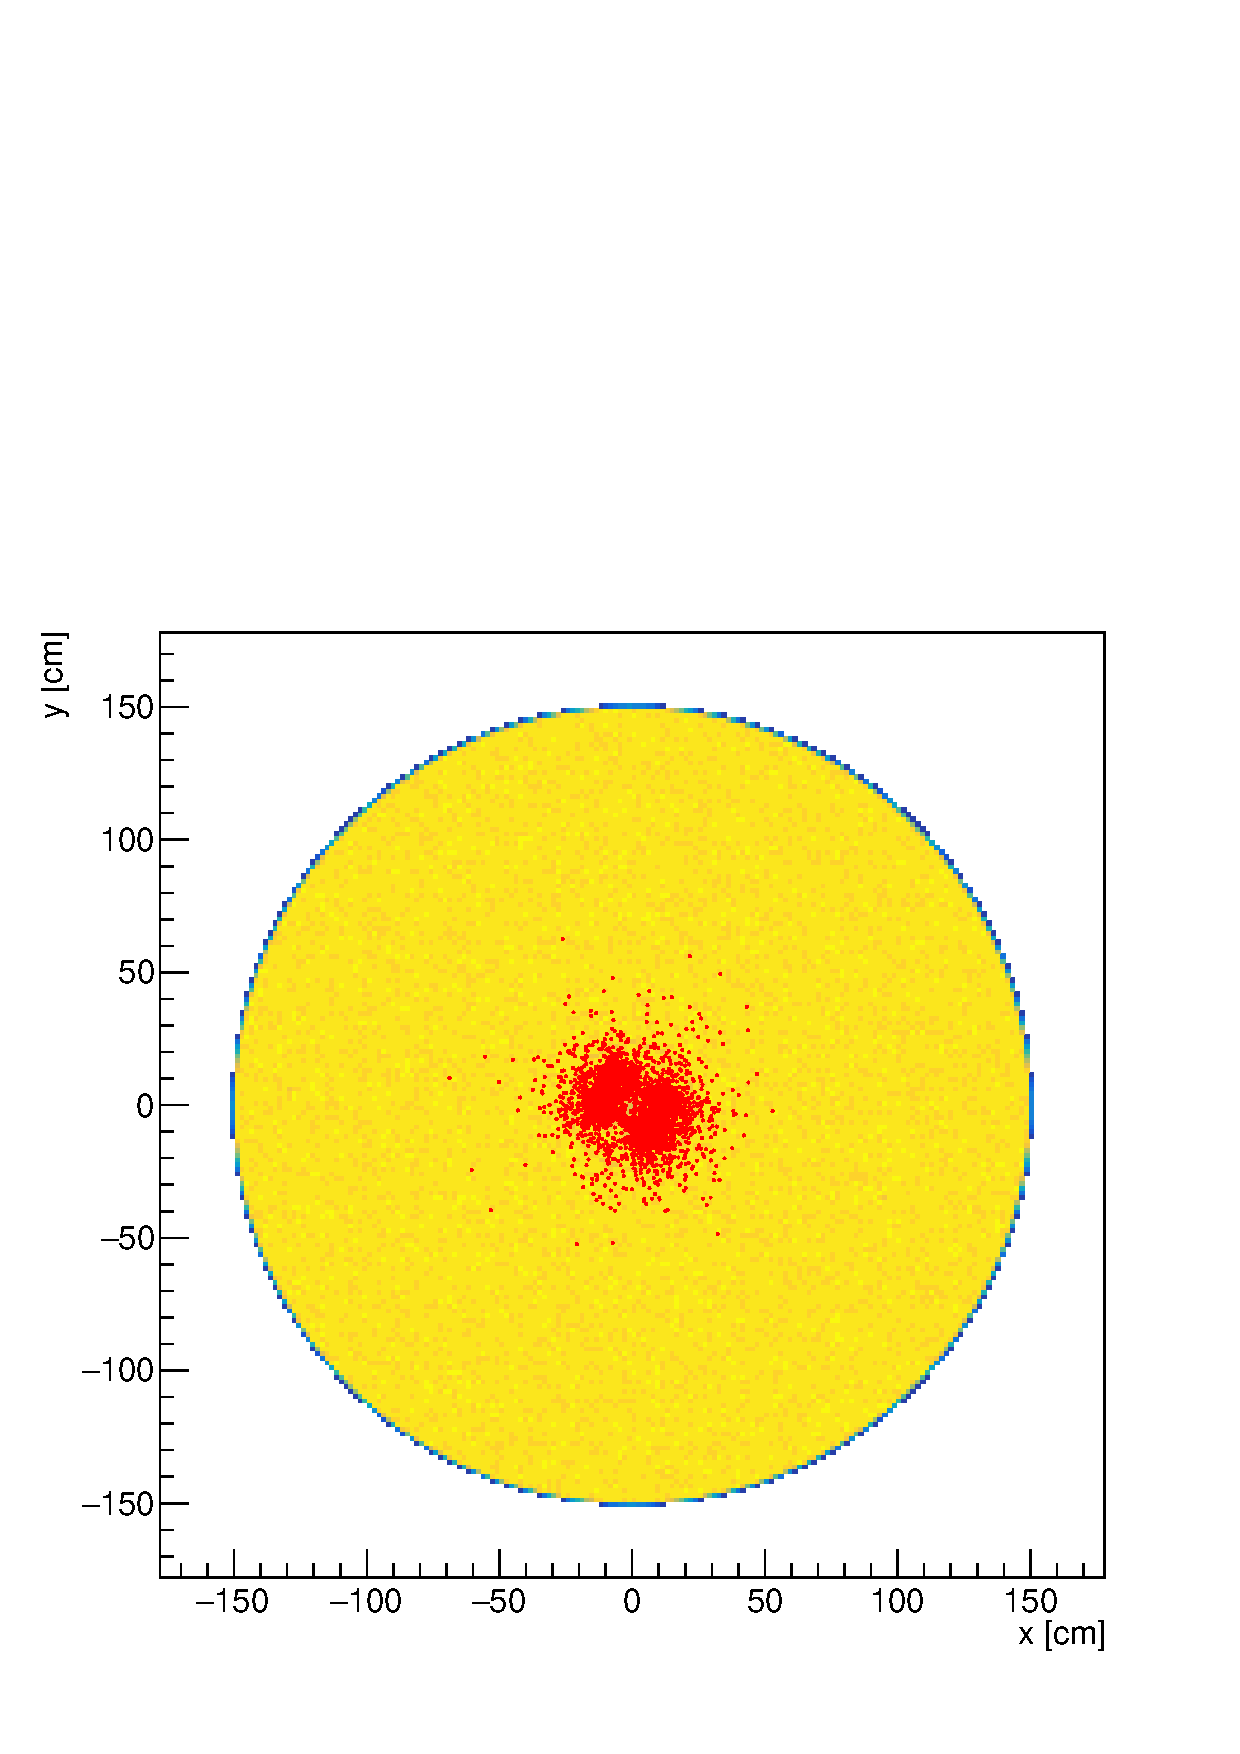
\includegraphics[height=75mm]{./Bilder/MC-Querschnitt-BEGes.pdf}
		\caption{Cross section from above}
		\label{fig:CrossSecAb}
	\end{subfigure}\hfill%
	\begin{subfigure}{.5\textwidth}
		\centering
		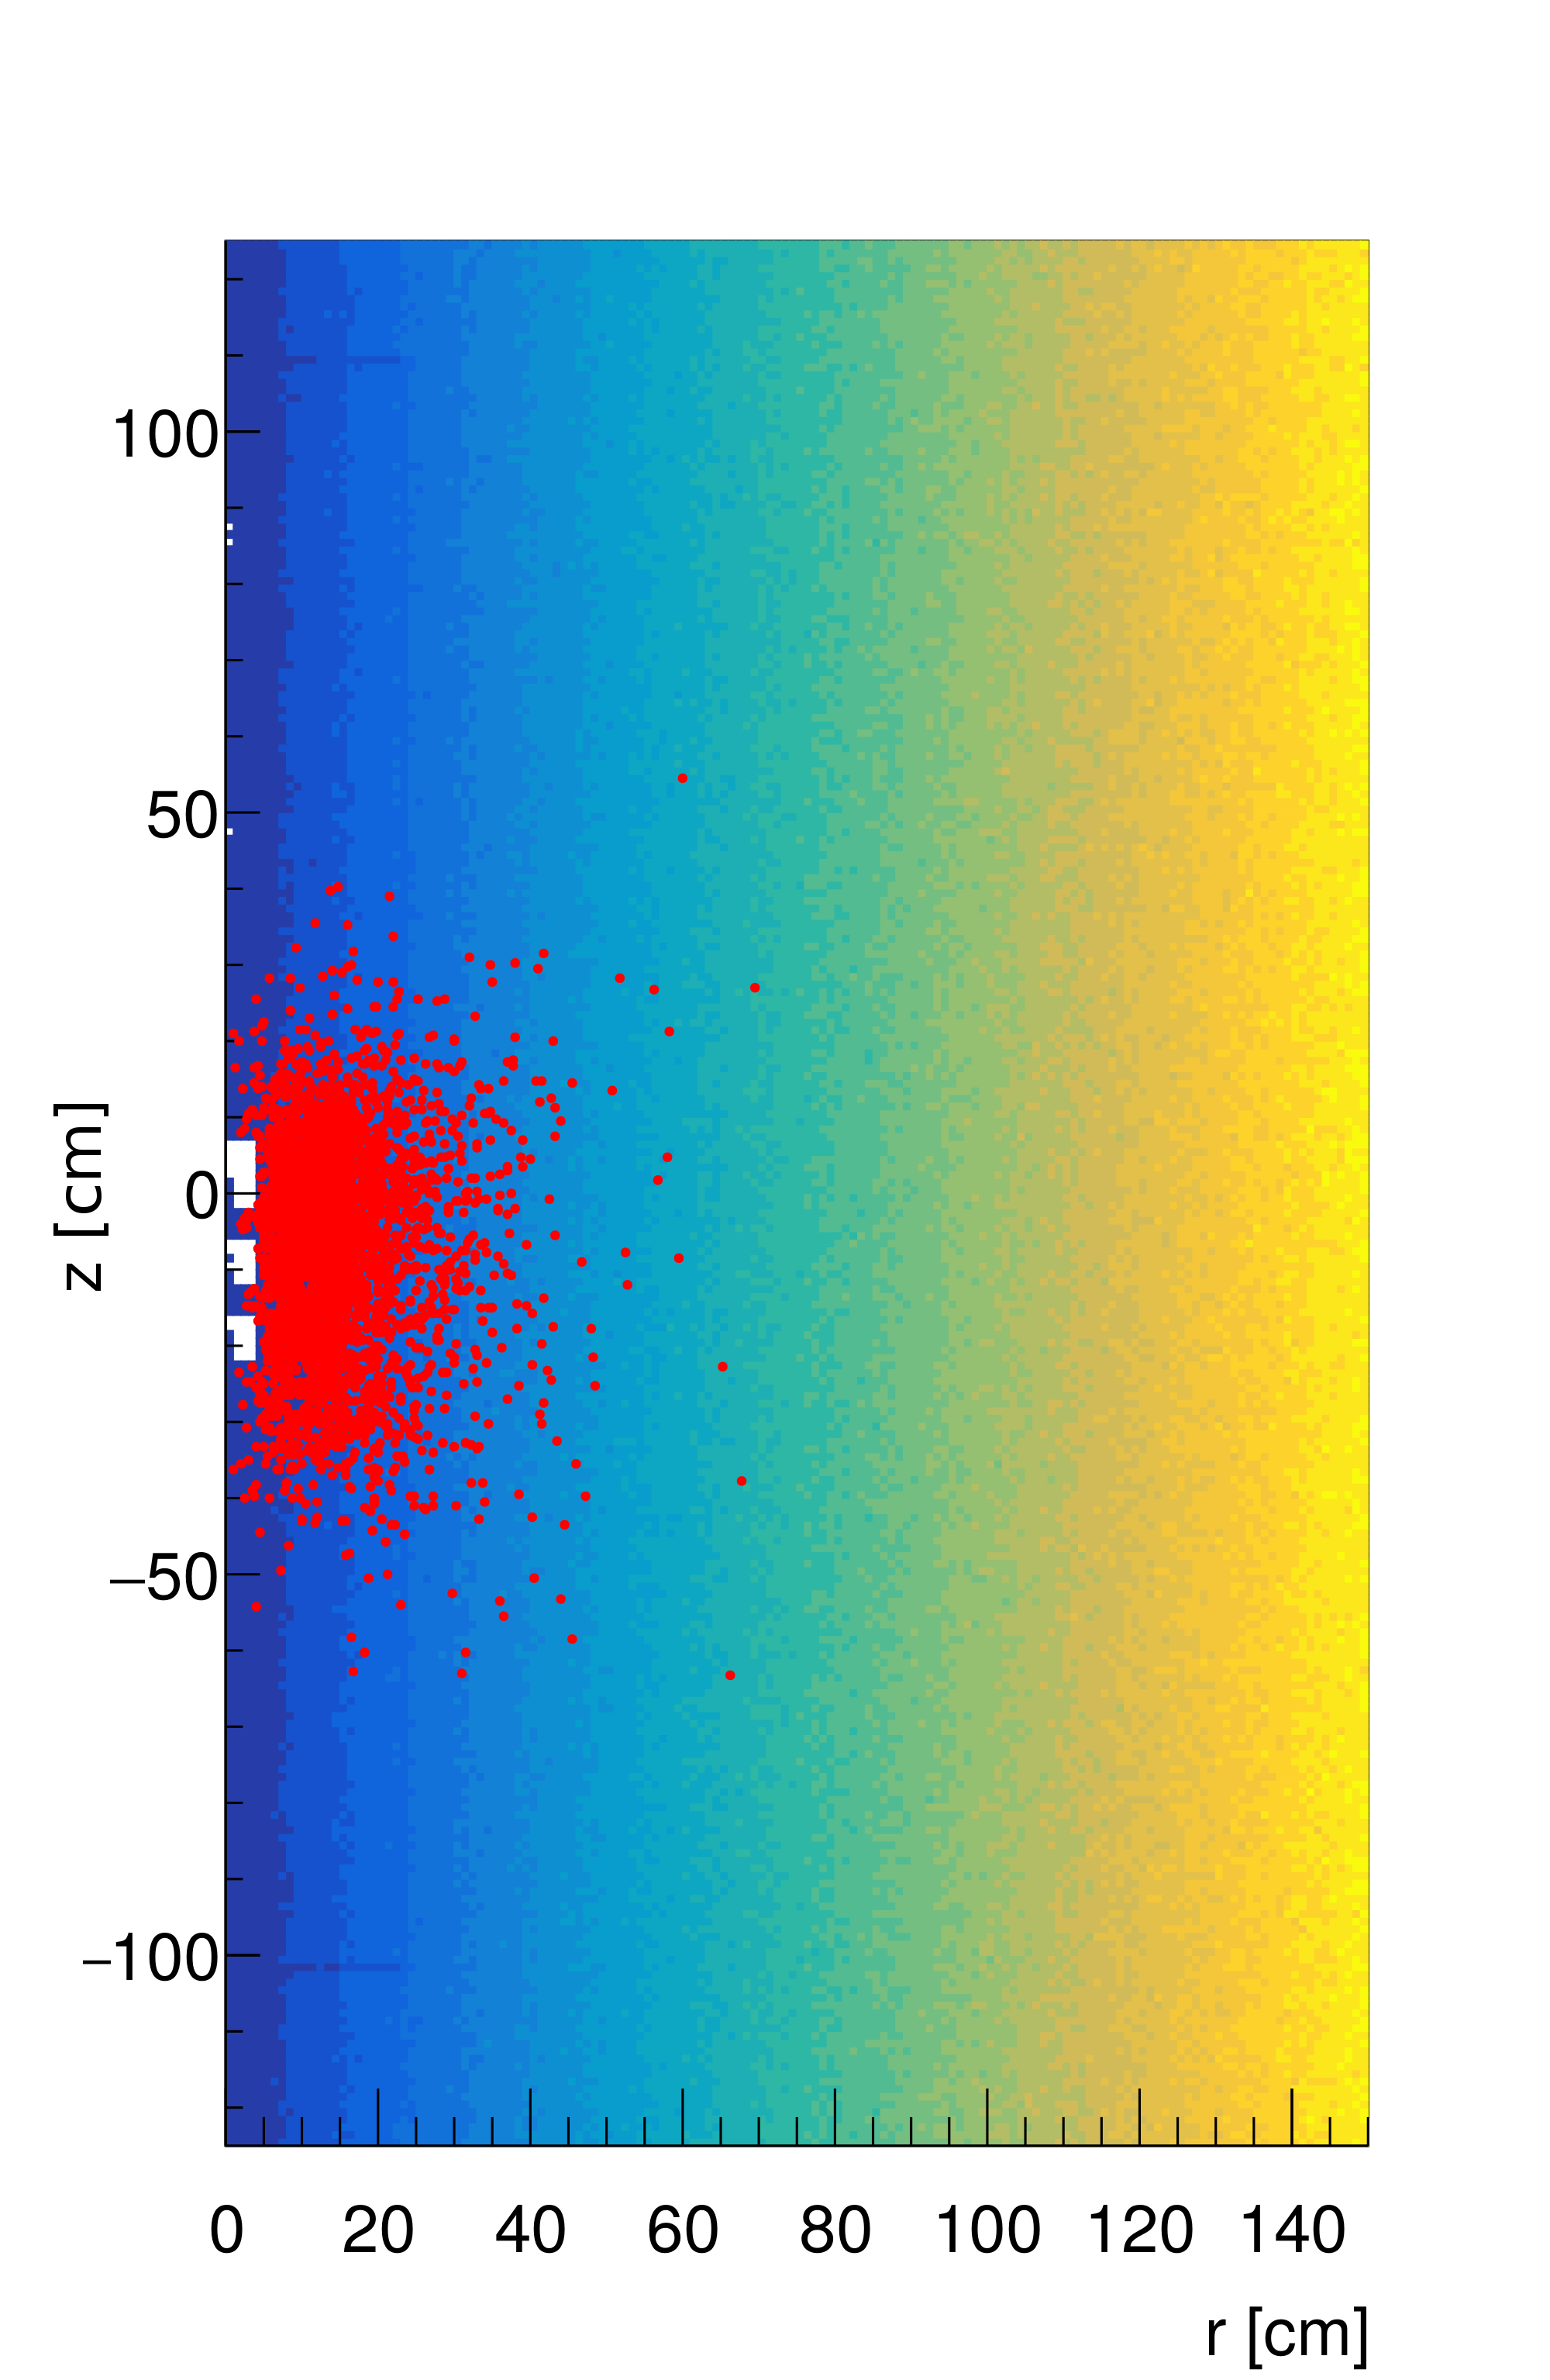
\includegraphics[height=75mm]{./Bilder/MC-Radius-BEGes.png}
		\caption{Radial cross section}
		\label{fig:CrossSecRa}
	\end{subfigure}
    \\
	\vspace{0.5cm}
    \caption{
    	The cross section of the simulated volume from above and radial.
    	The colored area shows the density of simulated decays. 
    	The red points indicate all events that were measured by BEGe detectors.
    	From it can be seen that photons that have been emitted far away from the detectors created no measurable signal in the detectors.
    	}
\vspace{0.5cm}
\end{figure}
\\

From these 50 million simulated decays with the anti-coincidence veto already applied only about 90 thousand have created a signal in a detector, only 30.465 of them in a BEGe and 24.902 in a COAX.
The spatial distribution of all measured events in the BEGe detectors can be seen as red dots in figure \ref{fig:CrossSecAb} and \ref{fig:CrossSecRa}.

\iffalse
From it one can see that the overwhelming majority of the detected events were positioned close to the detectors themselves.
At longer distances, the majority of all decays were no longer measured.
This means that, while holding the simulated decay density constant, the amount of measured events should not change when enlarging the volume.
But that would also mean that the detector efficiency $\epsilon$ would have a reciprocal proportionality to the simulated volume.
thereforee, one can expect the ratio $\frac{1}{\epsilon V_{\mathrm{sim}}}$ to be invariant with change of volume, provided that the volume is large enough.   
This is the reason why the usage of a smaller volume of LAr in the Monte Carlo simulation was justified.
This ratio easily be adapted to a conversion factor from the amount of measured counts in the 514keV line to the density of \Kr\ necessary to create the measured peak, just by dividing the ratio through the probability $p = 0.434\%$ of \Kr\ decaying into the excited state of \nuc{Rb}{85m}.
\\
\fi


\begin{figure}[t!]
	\centering
	\ifmakefigures%
	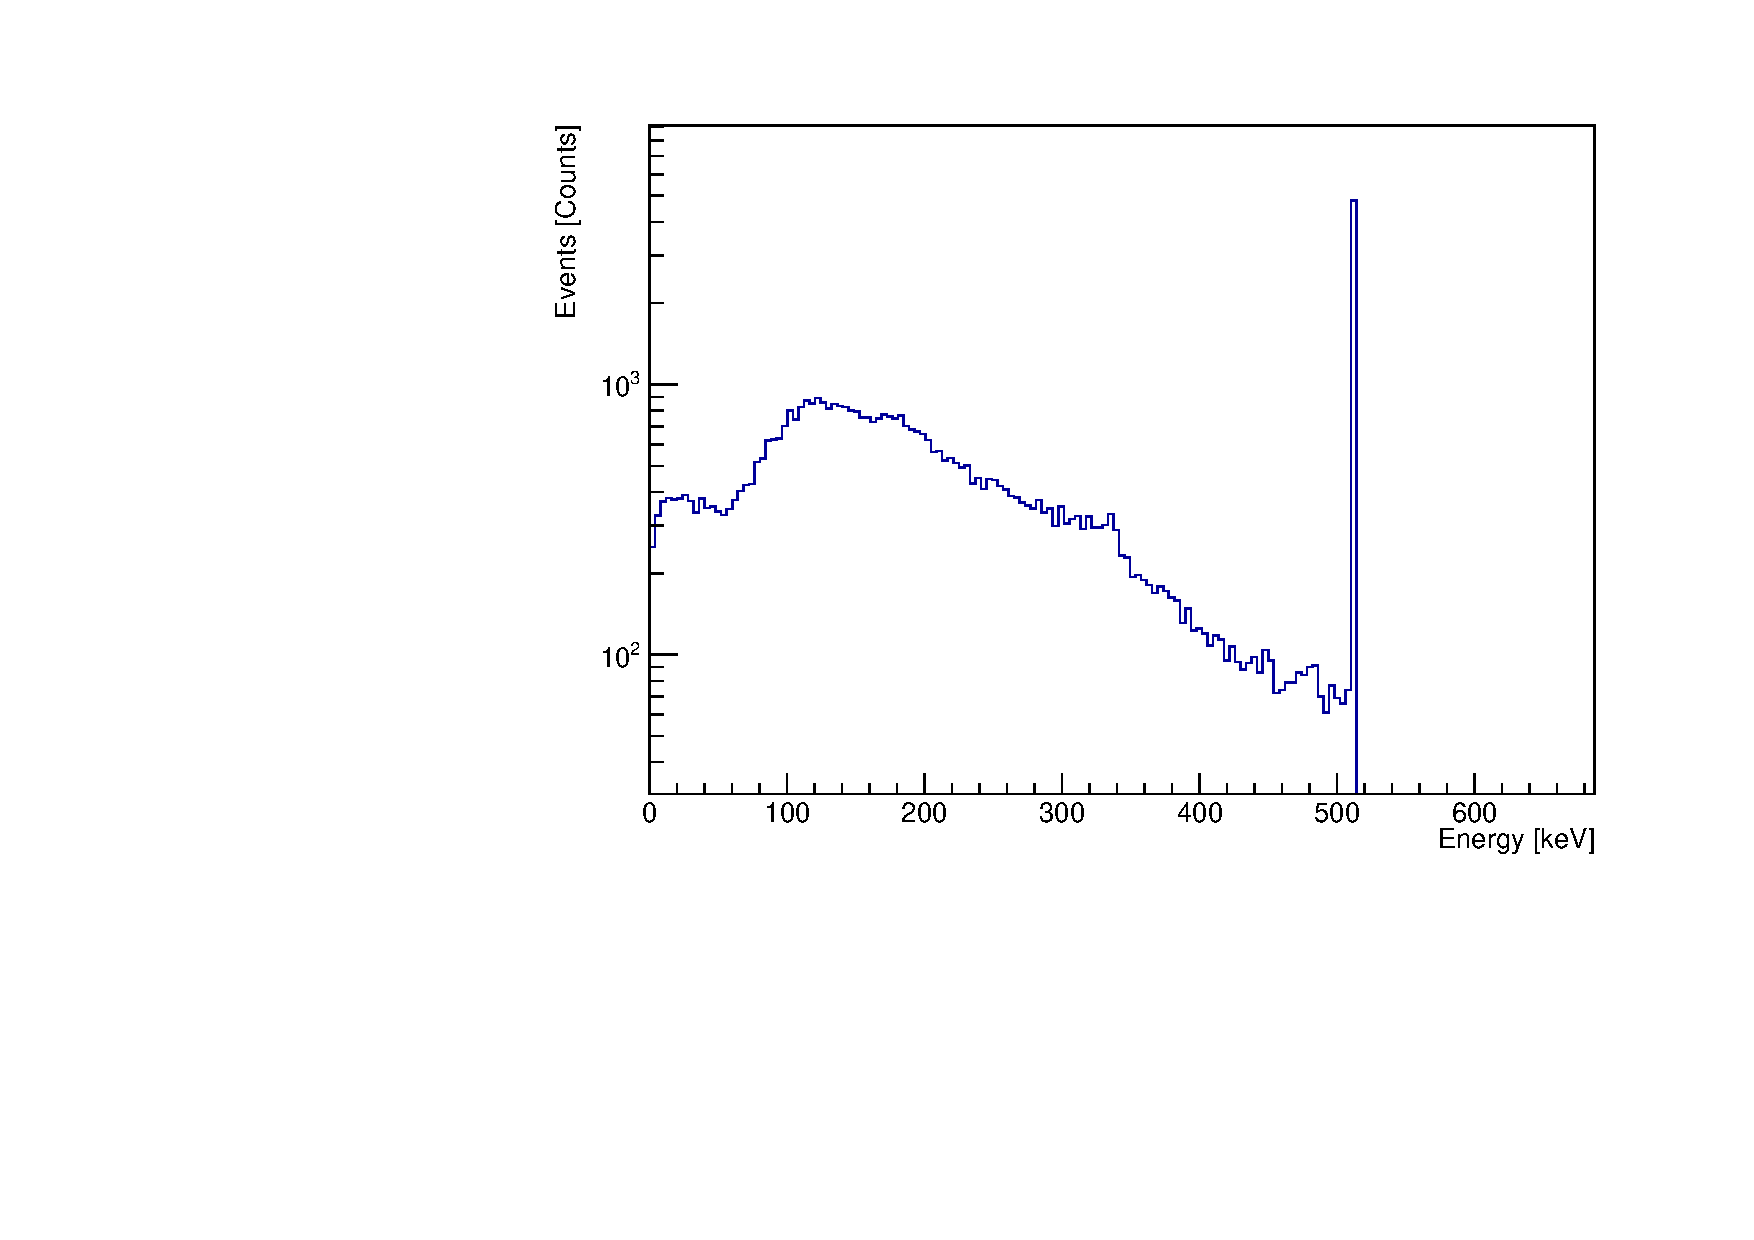
\includegraphics[width=100mm]{./Bilder/MC-514-Phasenraum.pdf}
	\fi%
	\caption{
    Energy spectrum of simulated events measured in BEGe detectors.
	The blue colored bin represents the counts used for determining the detector efficiency.
	The majority of measured signals had an energy below 514 keV.
	Among other things, the Compton peak at roughly 343keV can be seen.  
	}
	\label{fig:PhasenraumMC514}
\end{figure}


The spectrum of all the events detected in BEGe detectors is shown in figure \ref{fig:PhasenraumMC514}.
From it one can see that only a small amount cases the gamma deposited 514 keV in the detectors
The great majority of photons measured must scattered before they arrived in the detector or did not deposit all of their energy in them.
But to calculate the detector efficiency, only the measured events at the 514keV peak have to be accounted for.
In the BEGe detector spectrum the peak contains a total of \(\Delta N_{\mathrm{BEGe}} = 4511\pm67\) counts while the COAX peak contains  \(\Delta N_{\mathrm{COAX}} = 3706\pm60\) .
With a total of 50 million initial decays, this results in a efficiency of 
\begin{equation*}
\epsilon_{\mathrm{BEGe}} = \frac{\Delta N_{\mathrm{BEGe}}}{N_{\mathrm{sim}}} = (9.02\pm0.13) \times 10^{-5}  \frac{\mathrm{event}}{\mathrm{gamma}}
\end{equation*}
\begin{equation*}
\epsilon_{\mathrm{COAX}} = \frac{\Delta N_{\mathrm{COAX}}}{N_{\mathrm{sim}}} = (7.412\pm0.12) \times 10^{-5}  \frac{\mathrm{event}}{\mathrm{gamma}}
\end{equation*}
for the volume of the simulated cylinder.
This means that if a 514keV photon is emitted at any location in the liquid argon container, it has a probability \(\epsilon_{\mathrm{BEGe}}\) of being measured by one of the BEGe detectors.
On the other hand, it can also be said, that for every measured 514keV photon in one of the BEGe detectors an amount of about $1 / \epsilon_{\mathrm{BEGe}} = 10515$ \nuc{Rb}{85m} relaxations must occur.
In other words, the value $1 / \epsilon_{\mathrm{BEGe}}$ is a factor to convert from the measured entries to the actual amount of \nuc{Rb}{85m} relaxations.
\\

However, this value is direct proportional to the simulated volume $V_{\mathrm{sim}}$.
This dependency can be identified from figures \ref{fig:CrossSecAb} and \ref{fig:CrossSecRa}.
The red dots in them represent the location the measured gamma was released.
It can be seen that essentially all measured gamma originated in the immediate vicinity of the detectors.
This would mean that, with a big enough volume and a constant decay density $\rho_{\mathrm{dec}}$, the value $\Delta N$ of each detector remains constant under change of volume.
$N_{\mathrm{sim}}$ on the other hand is directly proportional to the volume due to definition of $N_{\mathrm{sim}} = \rho_{\mathrm{dec}} V_{\mathrm{sim}}$.
This results in a direct proportionality of $\frac{1}{\epsilon}$ with the simulated volume.
\\

A problem already mentioned above is that simulated that LAr volume $V_{\mathrm{sim}}$ was chosen smaller than it is in the actual setup. 
This makes it necessary for the wanted conversion factor to be volume independent.
But after $\epsilon$'s dependency with the simulated volume has already been determined, such a value can easily be generated by dividing $\frac{1}{\epsilon}$ through $V_{\mathrm{sim}}$.
This new value $\frac{1}{\epsilon V_{\mathrm{sim}}}$ is a conversion factor from the measured line count to the gamma emissions per liter.
By also dividing this new value by the probability $p=0.434 \frac{\mathrm{gamma}} {\mathrm{decay}}$, you finally get the desired conversion factor $\frac{1}{ p\epsilon V_ {\mathrm{sim}}}$ between the measured line numbers and the necessary \Kr\ decay density to generate this peak. 
 
\begin{equation*}
\frac{1}{ p \epsilon_{\mathrm{BEGe}} V_{\mathrm{sim}}} = (144.65\pm2.15) \frac{\mathrm{decay}}{\mathrm{event} \times l}
\end{equation*}
\begin{equation*}
\frac{1}{p \epsilon_{\mathrm{COAX}} V_{\mathrm{sim}}} = (176.07\pm2.90) \frac{\mathrm{decay}}{\mathrm{event} \times l}
\end{equation*}



\section{Mean measuring time}
\label{sec:CalcActiv}

The last remaining value to be determined is the mean measuring time $\bar{t}$ of all respective detectors.
The reason why not simply the entire duration of \PII\ was used as measuring time is due to the fact that not all detectors were recording all the time.
For determining this mean measuring time the exposures of all individual detectors has to be known.
An easy way to determine those values involves the test pulse signal.
Due to its periodicity of 0.05 Hz, the effective measurement times of the individual detectors can be determined by counting the number of measured test pulse signals in each detector and multiplying with the 20 seconds:
\begin{equation}
    t_\mathrm{i} = N_{\mathrm{TP}}(\mathrm{i}) \times 20\mathrm{s}
\end{equation}
The masses of the individual detectors are also known.
The individual exposures are therefore also easily determinable by applying 
\begin{equation}
    \varepsilon_\mathrm{i} = t_\mathrm{i} \times m_\mathrm{i}
\end{equation}
The combined exposure of all detectors of the same kind can then be calculated by adding up all of the exposures of the individual detectors.  
\begin{equation}
    \varepsilon_{\mathrm{comb}} = \sum_\mathrm{i} \varepsilon_\mathrm{i}
\end{equation}
The mean measuring times of the two detector types can then be determined by dividing their combined exposure through their combined masses. 
\begin{equation}
    \bar{t} = \frac{\varepsilon_{\mathrm{comb}}}{M} = \frac{\sum_\mathrm{i} N_{\mathrm{TP}}(\mathrm{i}) \times 20\mathrm{s} \times m_\mathrm{i}}{\sum_\mathrm{i} m_\mathrm{i}}
\end{equation}
By following this procedure the mean measuring times for the BEGe and the COAX detectors were determined to be
\begin{equation*}
    \bar{t}_{\mathrm{BEGe}} = 1.540 \unit{yr}
\end{equation*}
\begin{equation*}
    \bar{t}_{\mathrm{COAX}} = 1.803 \unit{yr}
\end{equation*}

These mean measurement times are exactly the times that each detector must have measured to obtain the same amount of combined exposure as from the actual measurement times.
Of course, this is only a simplification that generates a certain error.
Theoretically it would also have been possible to use the exposures of all individual detectors in the Monte Carlo simulation and determine how much a detector actually contributes to the detector efficiency.
However, this would have been too complicated and the error that results from the simplification can be neglected, since the measuring times of the individual detectors are almost always of the same sizes.
\\

\iffalse
The determination of the mean measuring time needs the exposures of the individual detectors.
Those values can be calculated by looking at how many test pule signals have been recorded by it ($N_{\mathrm{TP}}(\mathrm{i})$). 
Since the test pulse signals have been set to a frequency of $f_\mathrm{TP} = 0.05\unit{Hz} $ over the entirety \PII\, an effective measurement time can be calculated, by multiply the number of counted test pulse signals it by 20 seconds.
The individual effective measuring times are therefore given by
\begin{equation*}
    t_\mathrm{i} = N_{\mathrm{TP}}(\mathrm{i}) \times 20\mathrm{s}
\end{equation*}
where i is the index of the respective input channel of each detector.
\\

The second problem arises from the fact that the decay densities were  calculated with the assumption that one could merge all detectors of the same kind into one single detector.
This would mean that fro the remainder of the analysis one would be able to calculate as if the BEGe or the COAX detectors were only one detector respectively.
But now that the effective measurement times of each individual detector is supposed to be used, this assumption does not hold true anymore.
There are two different workarounds for this.
\\

In the first method another Monte Carlo simulation would be run, this time considering the amount of time each detector was actually measuring.
This would be very inefficient.
\\

The second method works around the merging problem by calculating an average measurement time for all detectors of one kind.
With this one could then calculate with the detector block as if they were such a single detectors.
This is very elegant solution because it is by far easier then running another simulation.
\\

For this average measuring time one has to consider the fact that a weigh on each individual detectors effective measuring time has to be applied.
This arises from the fact that every detector has an individual mass.
It is known, the detector efficiency of a single detector is directly dependent on its mass.
If one wants to combine all single detectors into one large detector, one has to consider that heavier detectors contribute more to the detector efficiency than lighter detectors.
It is therefore necessary to weight the measuring time of each detector with its individual mass.
But the multiplication of the individual measuring time of a detector with its mass are also the exposure the individual detectors.
This means that to calculate the mean measuring time, one just has to divide the combined exposure of all detectors of one kind through their combined mass.
\\

With this one can finally determine the mean measuring times using equation \ref{meanmeauringtime}.

\begin{equation*}
    \bar{t} = \frac{\sum_\mathrm{i} t_\mathrm{i} \times m_\mathrm{i}}{\sum_\mathrm{i} m_\mathrm{i}}
\label{meanmeauringtime}
\end{equation*}
From this, an average measurement time for the BEGes of $\bar{t}_{\mathrm{BEGe}} = (1.540\pm0.001)\unit{yr}$ and for the COAX of $\bar{t}_{\mathrm{COAX}} = (1.803\pm0.001)\unit{yr}$ can be calculated.
\\
\fi

With the mean measuring times, the line counts rates and the conversation factors the mean specific activity $\bar{a}$ of \Kr\ over the curse of all of \PII\ can  finally calculate by applying equation \ref{equ:activityDieErste}.
The resulting mean specific \Kr\ activities are
\begin{equation*}
    \bar{a}_{\mathrm{BEGe}} = (0.546\pm0.083)	\frac{\unit{mBq}}{\unit{l}}
\end{equation*}
and
\begin{equation*}
    \bar{a}_{\mathrm{COAX}} = (0.470\pm0.089)	\frac{\unit{mBq}}{\unit{l}}
\end{equation*}
These two values differ only inside their range of uncertainty.
From these two values an average specific \Kr\ activity for the whole period of \PII\ could then be calculated to
\begin{equation*}
\bar{a} = (0.508\pm0.086)\frac{\unit{mBq}}{\unit{l}}
\end{equation*}
\\
%5.07978E-04	8.57336E-05

\iffalse

One can now make some comparisons of this value with the WARP and the Darkside experiments.
In the case of the WARP experiment a specific activity of $(160\pm130)\frac{\unit{mBq}}{\unit{l}}$ \label{} was measured for the \Kr.
On the other hand, an specific activity of $(2.8577 \pm 0.18122) \frac{\unit{mBq}}{\unit{l}}$ was measured in the Darkside experiment.
The here determined value of $(0.508\pm0.085)\frac{\unit{mBq}}{\unit{l}}$ is about one order of magnitude smaller than the specific activity in the Darkside and whole three orders of magnitude smaller than the WARP experiment.
From these comparisons one can see, that the specific activity of \Kr\ in \gerda\ \PII\ seems to be much smaller than in other experiments using LAr.
\\

What one can also do is take the specific activities of the other two experiments and determine how many counts one would have been able to measure if the \Kr\ had their specific activity.
As simplification only the theroeticall values for the BEGe detectors was determined. 
How many counts the corresponds activity would induce in the BEGe detectors can be determined with the help of formula \ref{equ:correspondingEvents}.
\begin{equation}
\mathrm{N} = \bar{a} \times p \times \epsilon_\mathrm{BEGe} V_{\mathrm{sim}} \times \bar{t}
\label{equ:correspondingEvents}
\end{equation}
With the activity and the values determined from the analysis above one can calculate a corresponding amount of about 76152 events for the WARP experiment.
In the case of the WARP experiment one could expect the count rate to be much higher than the 183 events determined from the actual measurement.
For the Darkside experiment with an amount of 1360 counts is again about one order of magnitude higher than the here measured events.
From these comparisons one can see that for a much higher specific activity of \Kr\ to have actually been present a much bigger amount of events should have been counted.
As a graphical representation, the peaks that would have been able to be seen in the measured spectrum are displayed in figure \ref{fig:WARP} and \ref{fig:Darkside}.
\\

\begin{figure}[t!]
	\centering
	\begin{subfigure}{.5\textwidth}
		\centering
		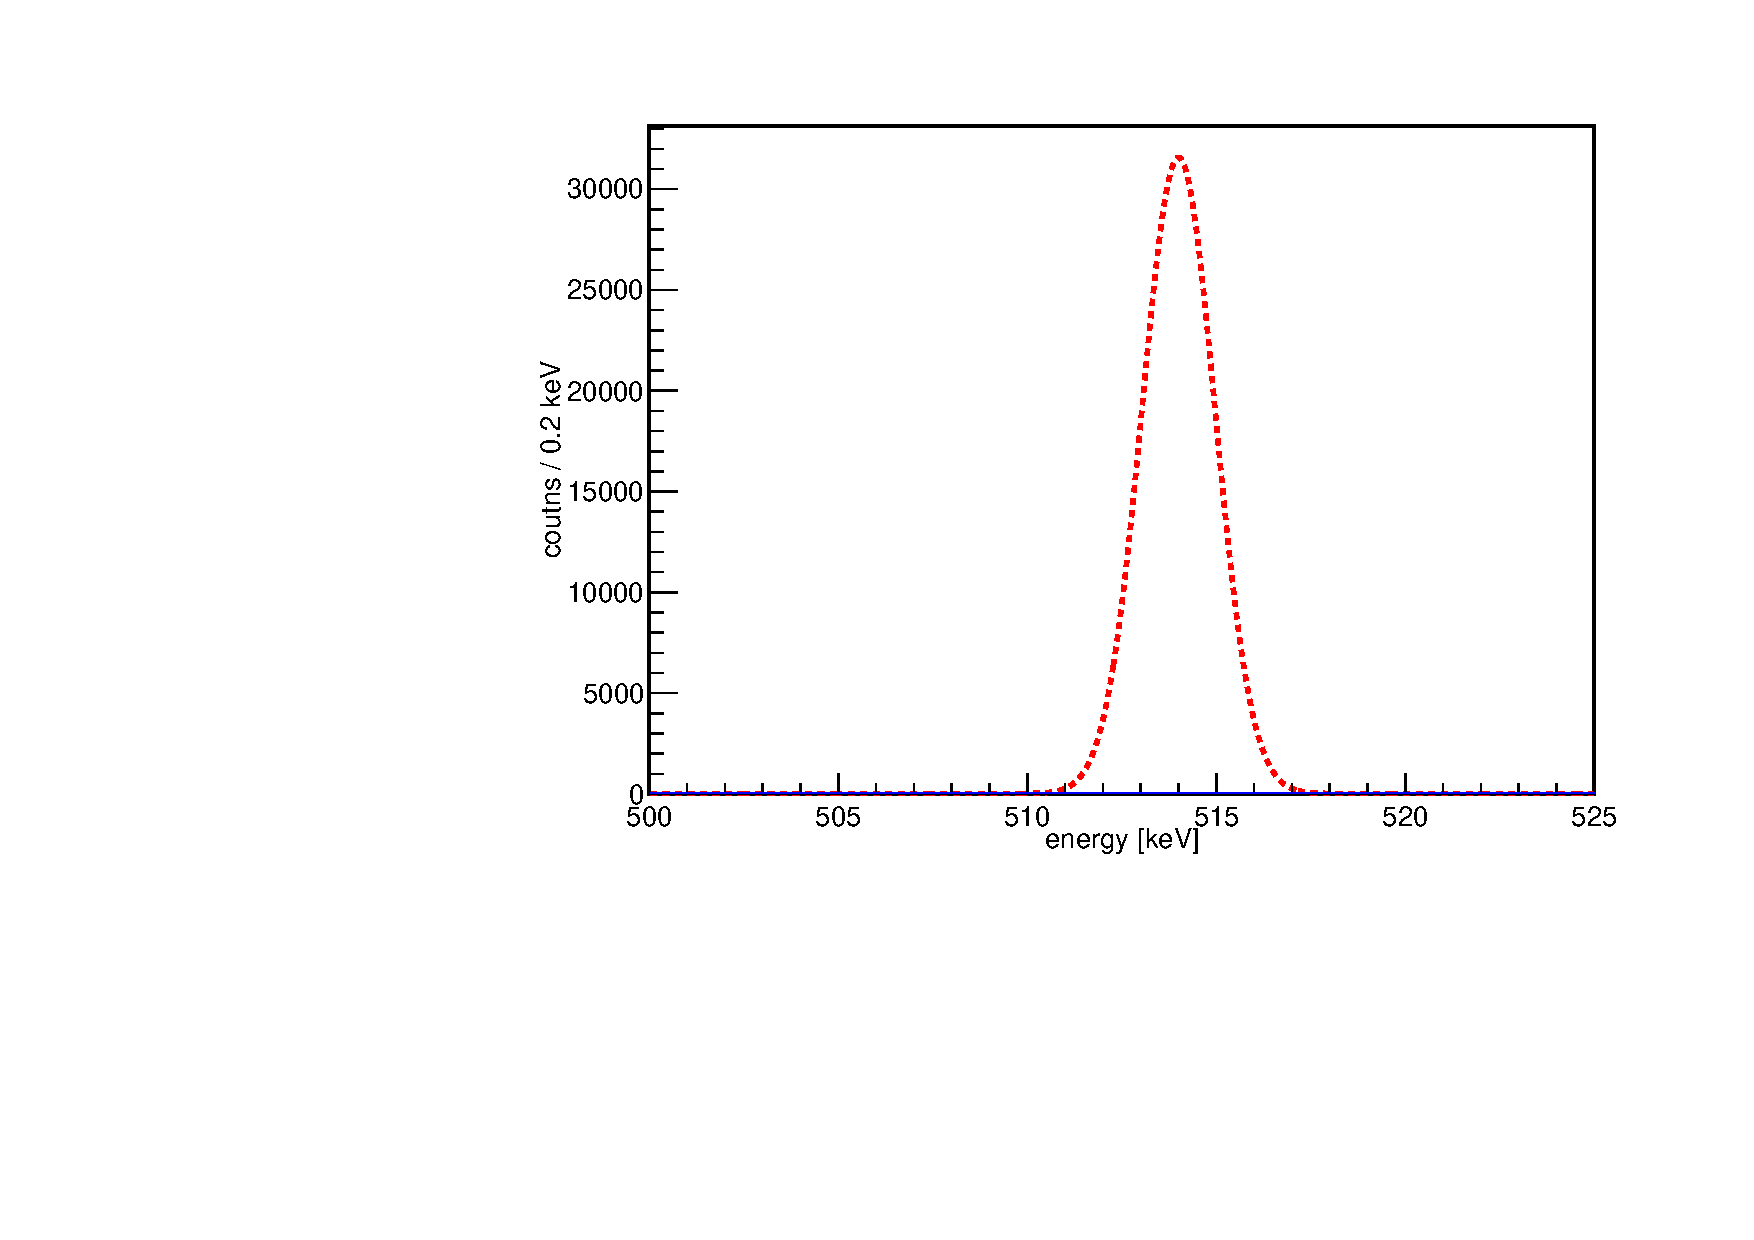
\includegraphics[width=75mm]{./Bilder/WARP.pdf}
		\caption{WARP}
		\label{fig:WARP}
	\end{subfigure}\hfill%
	\begin{subfigure}{.5\textwidth}
		\centering
		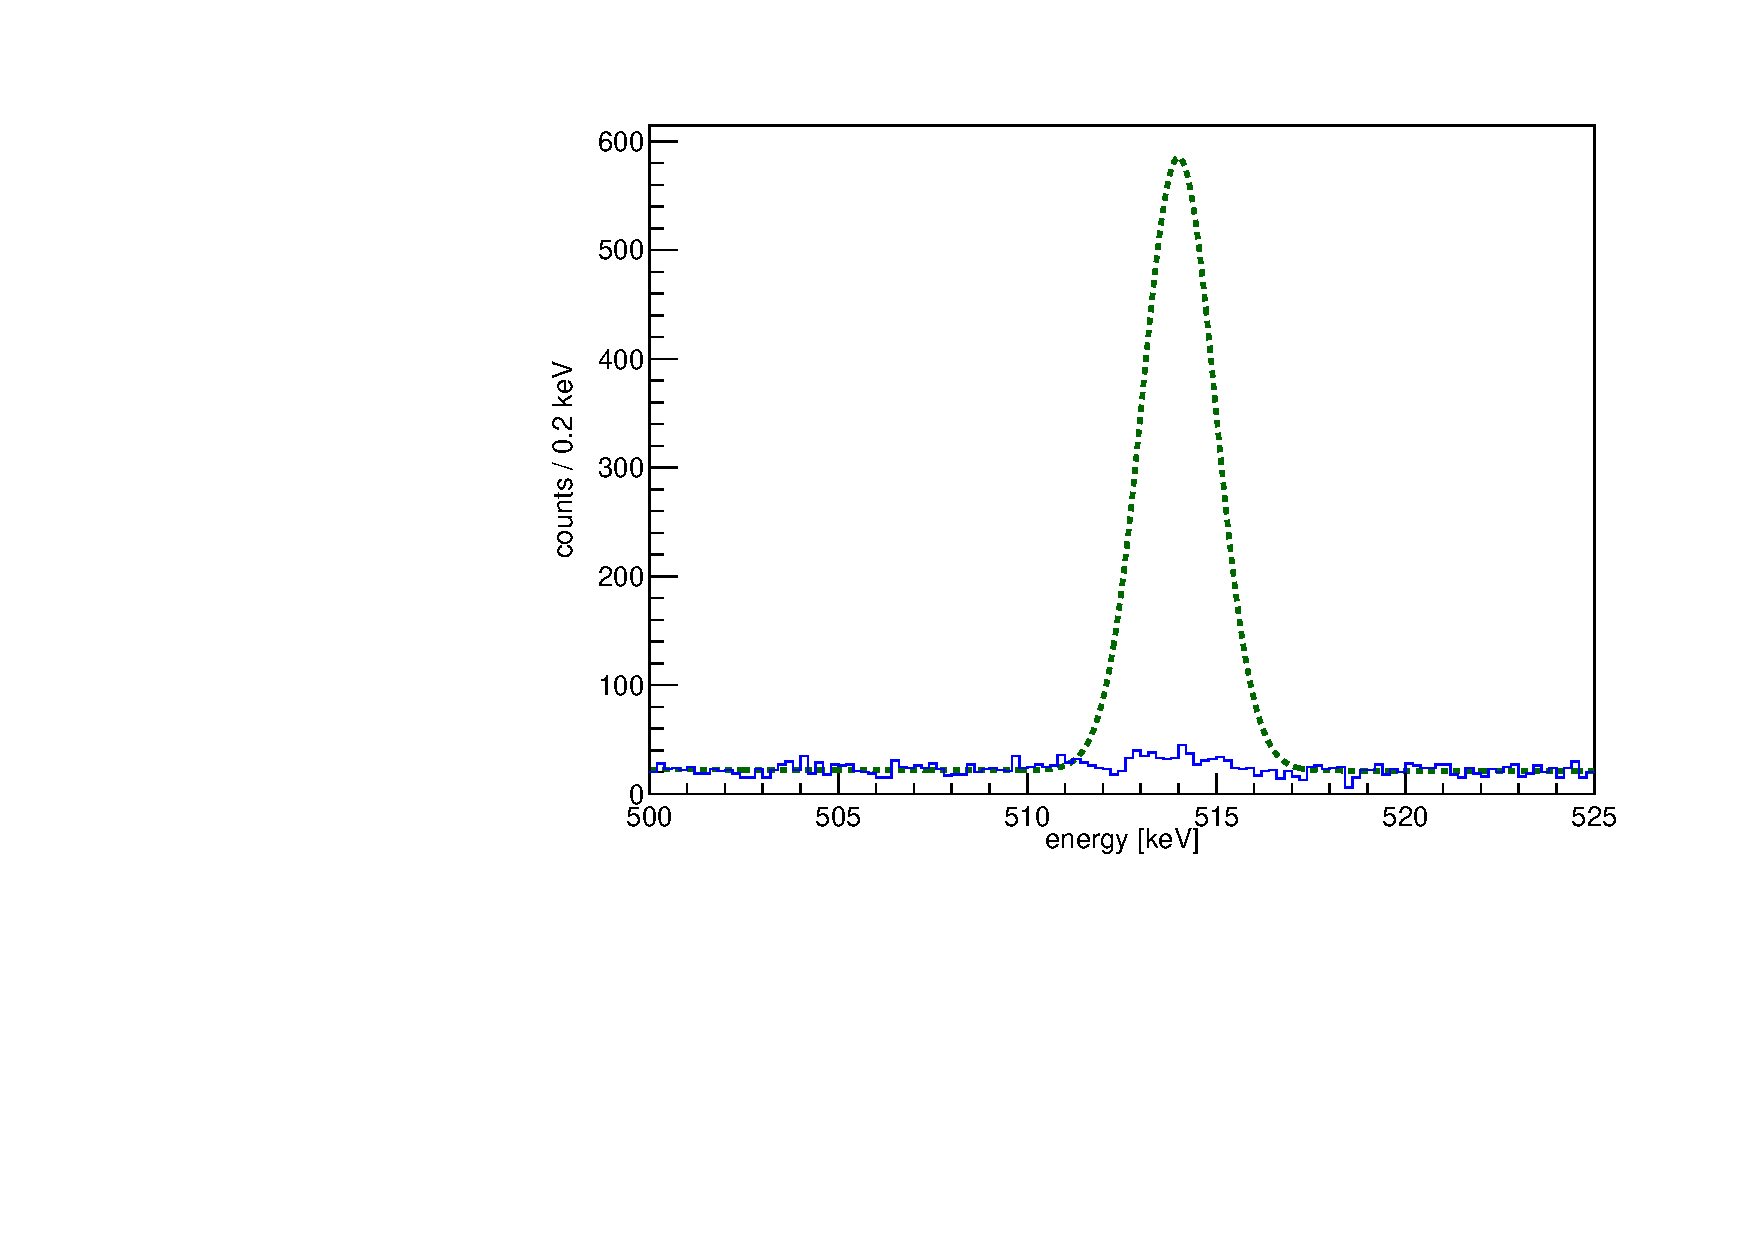
\includegraphics[width=75mm]{./Bilder/Darkside.pdf}
		\caption{Darkside}
		\label{fig:Darkside}
	\end{subfigure}
    \\
    \caption{
    	Energy spectra of the BEGe detectors from 500 to 525 keV.
    	The green plots in the spectra represent the theoretical peaks one could expect to measure if a specific activity of the respective experiment was present.
    	In both cases it would have created a much greater signal than observed above.
    	}
\end{figure}
\\

But why is the specific activity of \Kr\ in \gerda\ \PII\ so much smaller than in any other experiment?
As it was elaborated above, due to the argon being extracted from the atmosphere, \Kr\ should be present.
And the majority of the \Kr\ there should originate from nuclear power plants.
WARP's LAr also originated from the atmosphere but its specific activity was measured to be almost three orders of magnitude higher than \gerda's.
A possible explanation would be that the air from which the argon of WARP was extracted from was taken from a place with much a lot of nuclear power plants surrounding it while the argon of the \gerda\ experiment originated from air far away from any reactor.
On the other hand Darkside's argon originated from an underground reservoir where only natural fission decays produce any \Kr\.
But its specific activity is still much higher than \gerda's.
Also no extra purification of the LAr was applied.
This would mean that in the case of the LAr in \gerda\ one was extremely lucky to have found argon that had such low \Kr\ concentration that its impact on the background can basically be neglected.
\\

Now that a concrete value for the specific activity of \Kr\ has been determine the second attempt to measure the specific activity will described in the next chapter.
\\  
\fi



%	4.70E-04	8,87E-05	Bq/l


% calculate Amplitude of Gauss peak at 514keV and use factor from Monte Carlo Simulation to estimate

% look at phase diagram at range of 500 to 525 keV, use different filters and fit remaining data with Gaussian function
% -> get amplitude
% make a Monte Carlo simulation to estimate actual Kr85 activity in LAr from measured activity in detectors
% -> with amplitude and factors from MC-Simulation one can calculate the specific activity

\chapter{Change in Count Rate over Time}
\label{sec:SAfromDecrease}

As described in the beginning of section \ref{sec:SAfrom514}, the line count analysis method of the rare \Kr\ decay was expected to be relatively precise.
By following this procedure we were able to determine the activity down to the order of 10$^{-4} \frac{\mathrm{Bq}}{\mathrm{l}}$ with reasonable uncertainty.
This chapter will now concentrate on implementing and discussing the second approach of determining the specific activity by using the change in count rate over time.
This method does not rely on any of the values used in the line count rate analysis which is why this approach is truly independent of the other method.
Ideally, a similar result from this method would confirm the specific activity determined in the previous chapter. 
\\

But compared to the line count rate analysis is the second method  expected to be relatively imprecise.  
This estimation comes from the fact that this method relies on a the approximation, that \Kr\ is the only radioactive isotope in the \gerda\ setup that has a non negligible change in its specific activity.
The idea is that \Kr\ has the lowest half-life (T = 10,739\unit) of all other remaining radioactive isotopes in liquid argon and therefore only \Kr\ should change its decay rate.
In comparison, other radioactive isotopes that are of interest are \nuc{Ar}{42} with a half-life of 32.9 y \cite{chen_nuclear_2016}, \nuc{Ar}{39} with 269 y \cite{singh_nuclear_2006} and \nuc{Po}{210} with 138d \cite{kondev_nuclear_2008}.
\\

Even though\nuc{Po}{210} has a much lower half life than \Kr, the mean energy of the escaping alpha particle is much higher than the mean beta energy of all of the isotopes above.
This is important because in the course of this chapter it is explained that only those events are considered in the analysis which have deposited an energy between 200 and 400 keV. 
This means even though \nuc{Po}{210} has a much lower half life it would not create much of a change in count rate in the investigated interval due to its much lower probably to release an alpha particle in this energy range.
\\

The two different types of argon isotopes have both a mean beta energy close to \Kr's 251.59 keV.
Their change in event rate should therefore be measurable in the investigated interval.
The change in activity of \nuc{Ar}{39} can be neglected because its half life is one order of magnitude larger then \Kr's.
\nuc{Ar}{42} on the other hand has a half life that is in the same order of magnitude as \Kr.
But its specific activity has already been determined to be about $148\mathrm{\mui Bq/l}$ \cite{becerici_schmidt_results_2014} which is about factor 3.5 smaller than the expected \Kr\ specific activity.
Whether or not one have to consider the influence of this isotope will be discussed later in this thesis.
For now the simplification will be applied that its change will be much smaller than \Kr's so that one can neglect it.
\\

All other radioactive isotopes that are residual in the liquid argon have either a much longer half life than \nuc{Ar}{42}, their mean beta energy is much higher than 400keV or their specific activity is too small too small to measure any kind of change over time.
It can thereforee be assumed that all changes in intensity are only due to \Kr\ decay.
Even if the specific activity determined with this method is not expected to be as precise as the first method, it can still be used as a crosscheck for the other specific activity determined above.
\\

It has now been shown that this approach can be applied in the case of \gerda\ \PII\.
thereforee it is now necessary to discuss how exactly the specific activity can be determined by changing the intensity.
To measure the change in count rate every measured event will have to be drawn over time in a fit function and through the resulting plot an exponential fit applied.
From the amplitude of the resulting exponential function a count rate $R_{\mathrm{count}}$ of counts per second can be determined.
\\

To calculate the specific activity of \Kr\ with this value one again has to use a Monte Carlo simulation to calculate a conversion factor between those values. 
One cannot use the same simulation from the first method because in this case actual \Kr\ decays have to be simulated, not only the emission of 514keV photons as it was done in the prior chapter.
That is why another Monte Carlo simulation has to be carried out.
With it a new conversion factor $\frac{1}{\epsilon V_{\mathrm{sim}}}$ between the measured counts and the decays necessary to create this amount of counts can be determined.
\\

Finally the specific activity can be calculated from these two values.
\begin{equation}
a(t=0) = \frac{R_{\mathrm{count}}}{\epsilon V_{\mathrm{sim}}}
\label{equ:ActivityDieZweite}
\end{equation}
It is important to note that this approach determines the specific activity of \Kr\ at the start of \PII\ while the first method calculates the mean specific activity over all of \PII.
To compare those two results, in the end a mean specific activity of the second method has to be determined.
The following sections will focus on the concrete implementation of this method and the values determined by them.
\\

\section{Event Rate}
\label{sec:EventAct}

\begin{figure}[t!]
	\centering
	\begin{subfigure}{.475\textwidth}
		\centering
		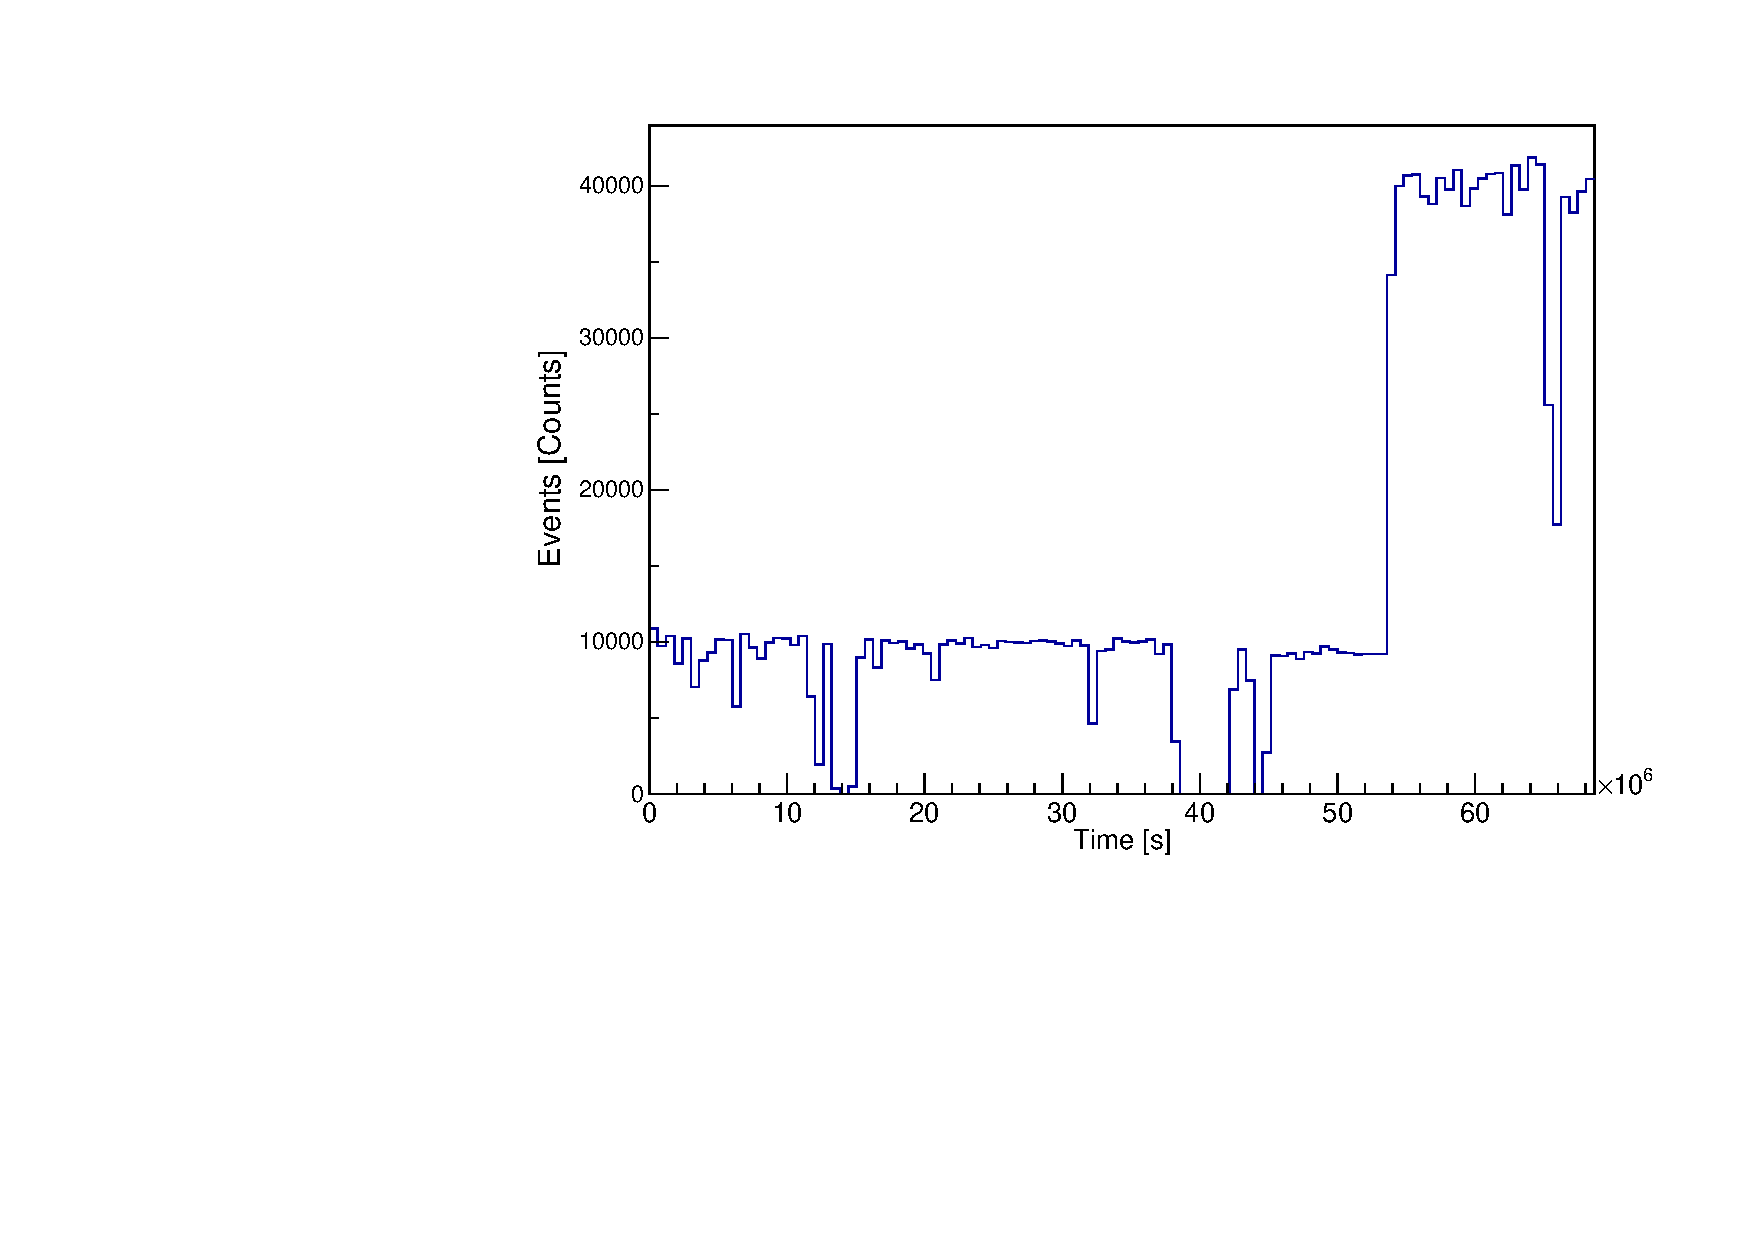
\includegraphics[width=\textwidth]{./Bilder/ZeitverlaufALLE.pdf}
		\caption{every event}
		\label{fig:ZeitAll}
	\end{subfigure}\hfill%
	\begin{subfigure}{.475\textwidth}
		\centering
		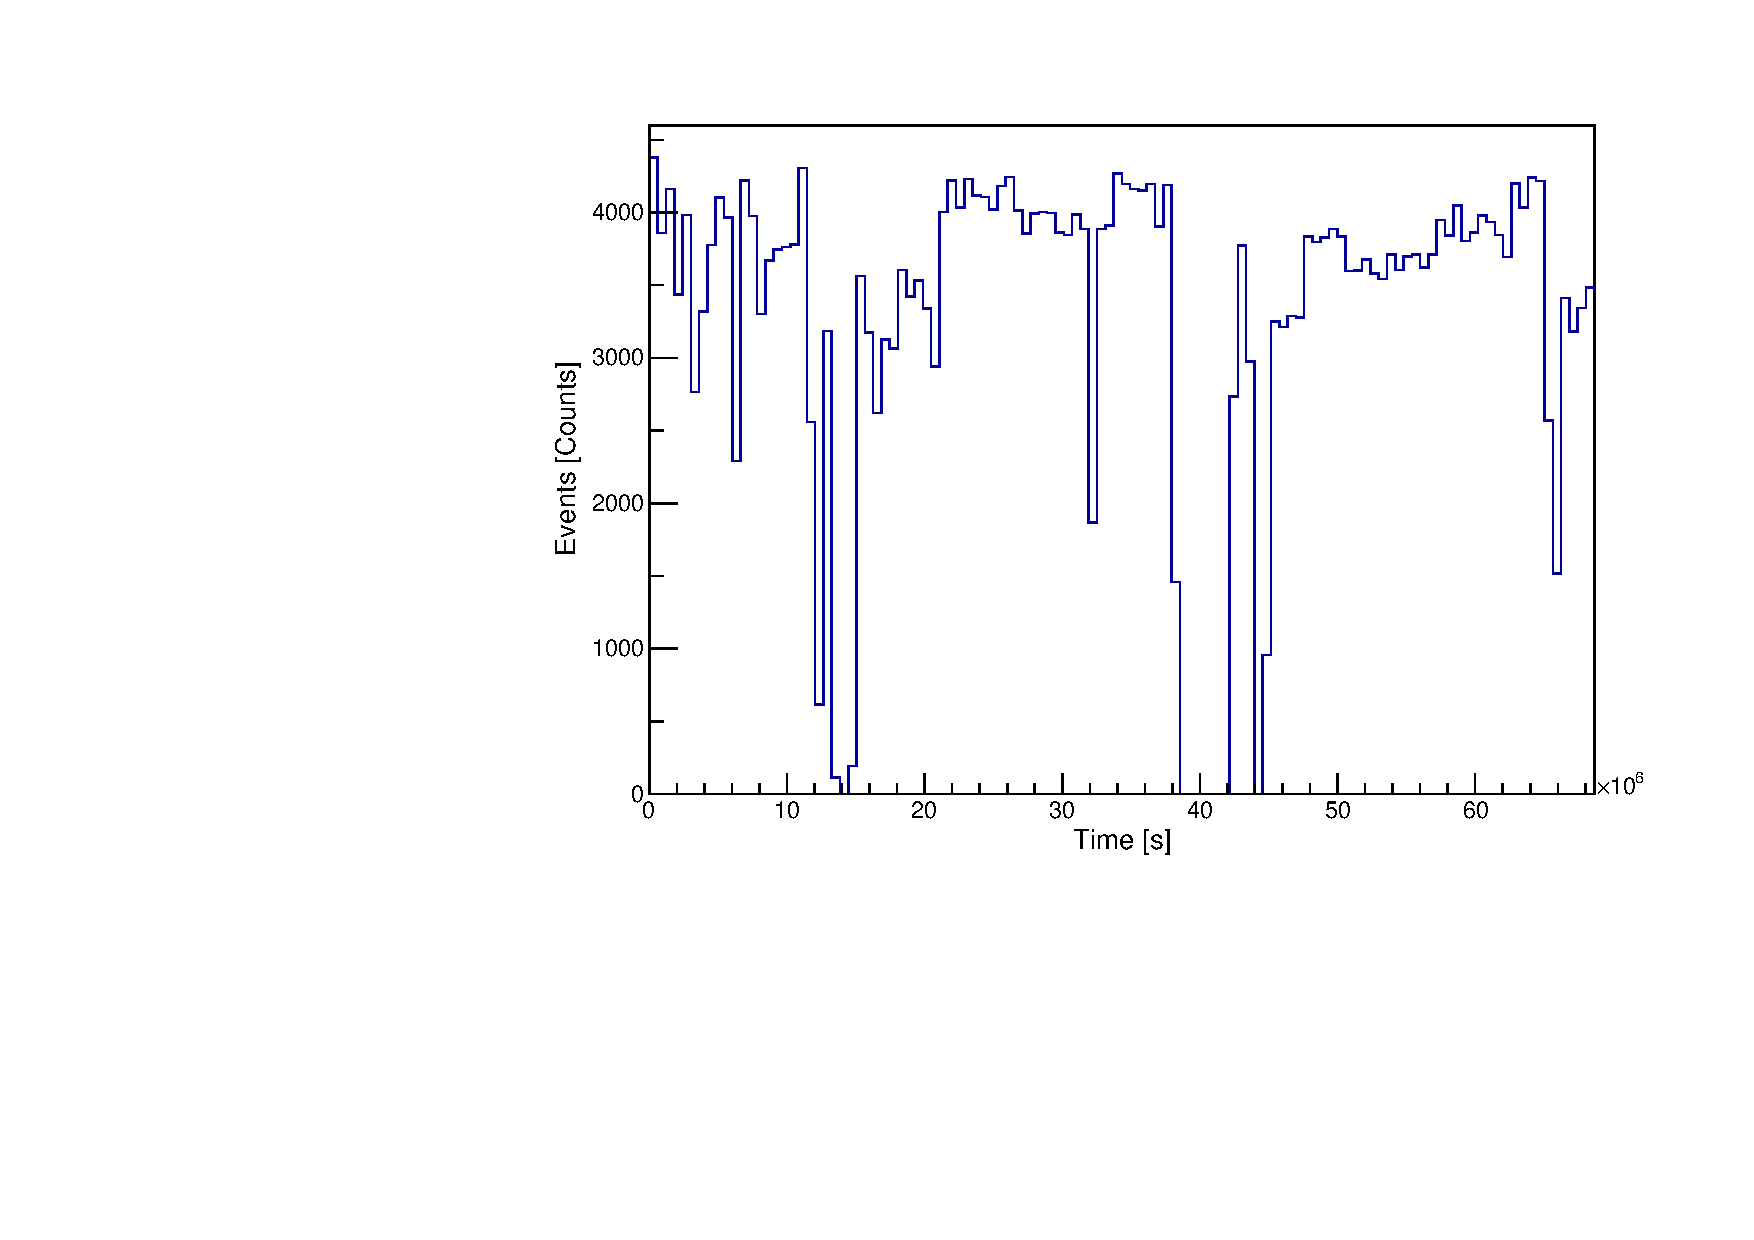
\includegraphics[width=\textwidth]{./Bilder/ZeitverlaufLimits.pdf}
		\caption{only energies between 200 and 400keV}
		\label{fig:ZeitLimits}
	\end{subfigure}
    \\
    \caption{
    	The change of count rate over time. 
    	In both figures the amount of events measured in one week are plotted over the whole time frame of \PII. 
    	In figure (a) no filters were imposed onto the used events while in (b) only those events were used that have an energy between 200 and 400 keV. 
    	One can see that further precautions must be taken before an exponential decrease can be determined. 
    	}
\end{figure}

To determine the change of count rate with time one has to plot the amount of measured events over time in a histogram with a suitable binning (see figure \ref{fig:ZeitAll}).
In this case a binning of one week per bin was chosen which results in about 114 bins for the 2.17 years of \PII.
As in the line count rate analysis, histogram \ref{fig:ZeitAll} only used events where the Muon veto and the detector anticoincidence veto were not triggered.
When looking at the histogram two new problems seem to occur.
Firtsly, there seems to be a great jump in the amount of events measured in the second half of \PII.
And secondly, there are times in which the amount of events measured drop to zero.
These two discontinuous changes to the expected exponential decrease make it impossible to lay an exponential fit function throug the graph.
It is therefore necessary to find a way to suppress them.
But for this to be done one has to investigate where these discontinuities originate from.
\\

Firstly, we discuss the big jump in number of events measured.
This jump originates from the lowering of the energy threshold on the 12.10.2017.
This reduction of the lower threshold dramatically increased the number of events measured.
Due to every detector having different characteristics, the limit was set for each detector individually.
Before the lowering the highest limit was set at about 140keV for the BEGes and at 185 for the COAX.
After the lowering all event with an energy of at least about 15keV could be recorded by all detectors.
For a graphical representation, see the beginning of the spectra in figure \ref{fig:before} for all events measured before and figure \ref{fig:after} for all events after the lowering of the limit. 
This means that from the 12.10.2017 on a much higher event rate was measured just because more event were actually recored.
To work around this continuity problem all one has to do is limit the events used for the analysis to those that have a minimal energy of about 200keV. 
While doing so one can also set up an upper limit on the energy.
Its purpose is to suppress events caused by isotopes with a much higher  mean energy than \Kr.
Even though they should only create a constant background, not considering \nuc{Po}{210}, but their presence make a change in intensity harder to identify.
therefore was 400 keV chosen as an upper limit for the event energy.
Theoretically the endpoint energy of \Kr\ is at 687keV, but its count rate towards the endpoint is that low that one would basically only include more constant background by setting the upper limit higher.
A new plot including only events between the energy limits of 200 and 400keV can be seen in figure \ref{fig:ZeitLimits}.
\\
\begin{figure}[t!]
	\centering
	\begin{subfigure}[t]{.475\textwidth}
		\centering
		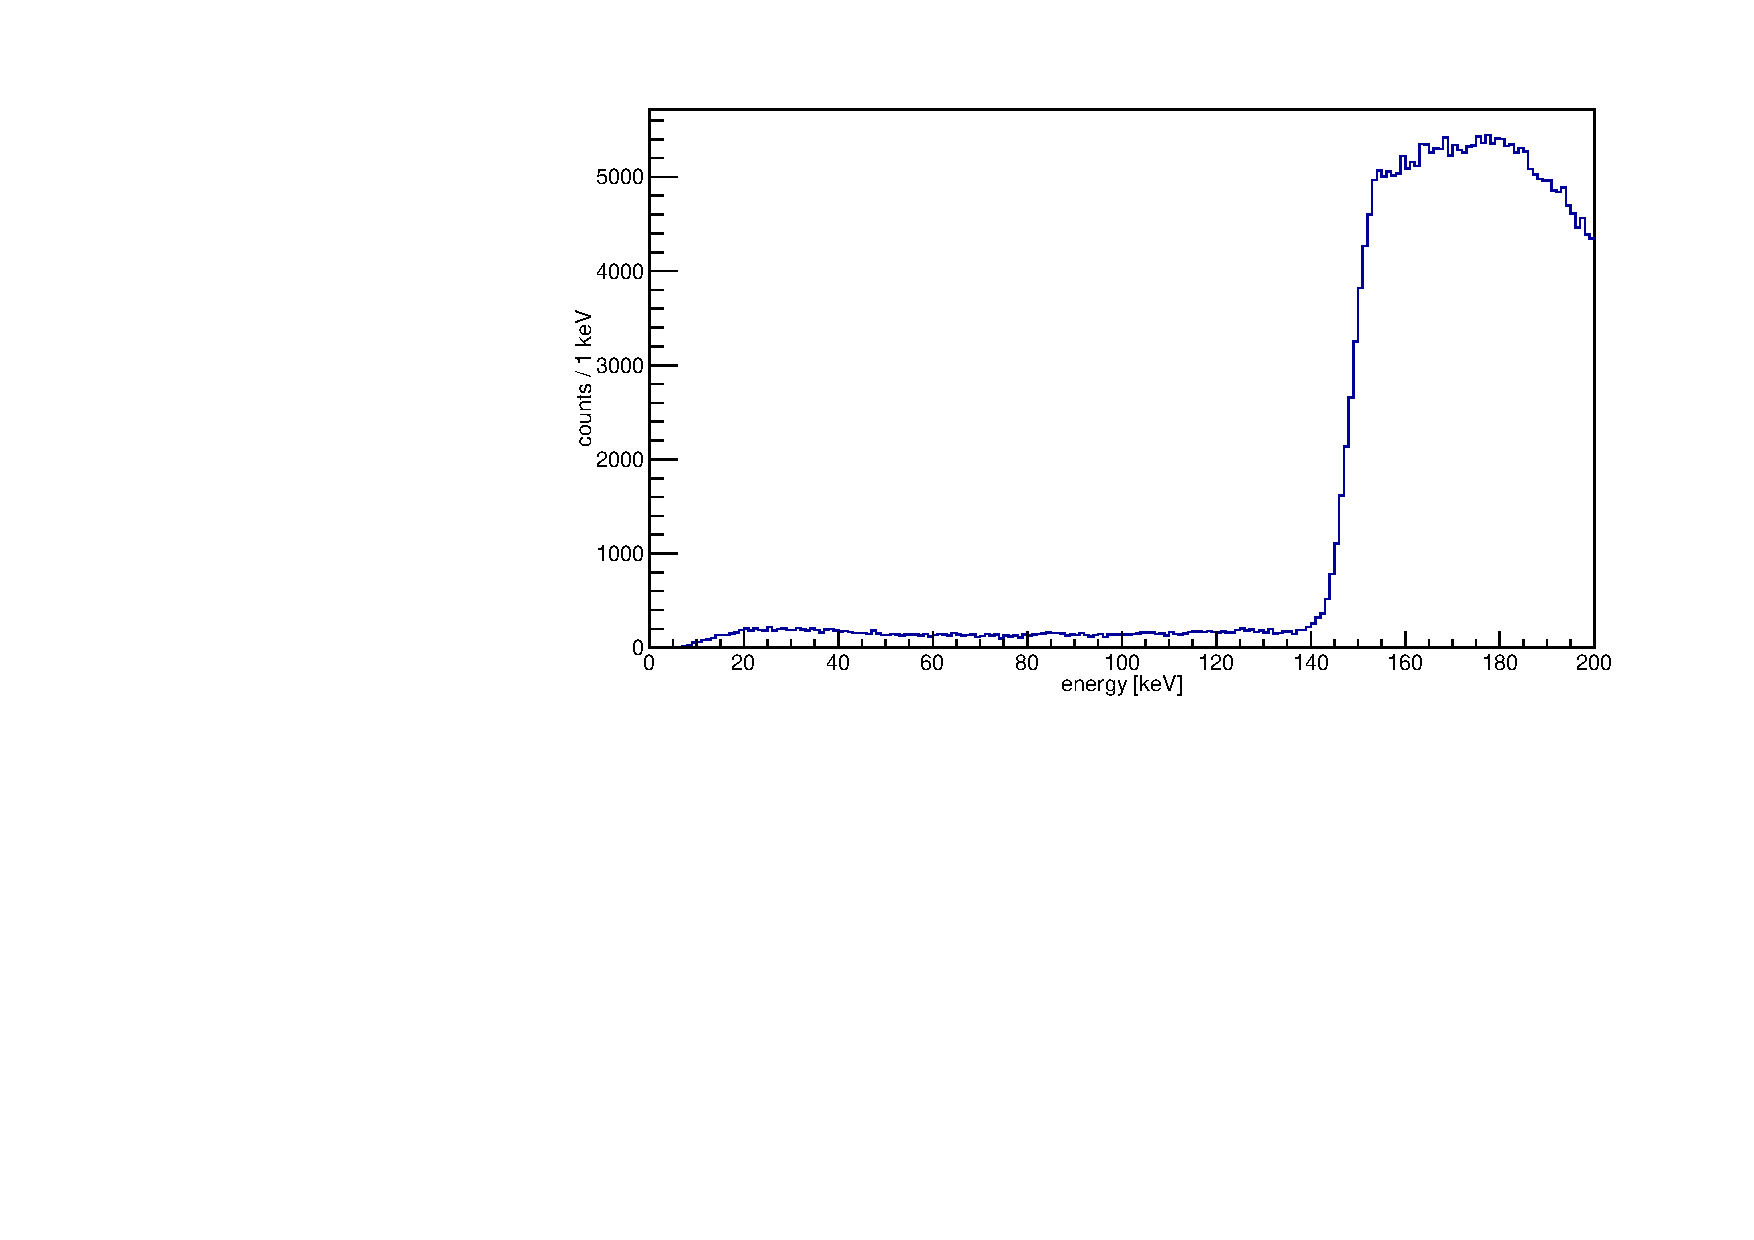
\includegraphics[width=\textwidth]{./Bilder/beforeTheFall.pdf}
		\caption{before}
		\label{fig:before}
	\end{subfigure}\hfill%
	\begin{subfigure}[t]{.475\textwidth}
		\centering
		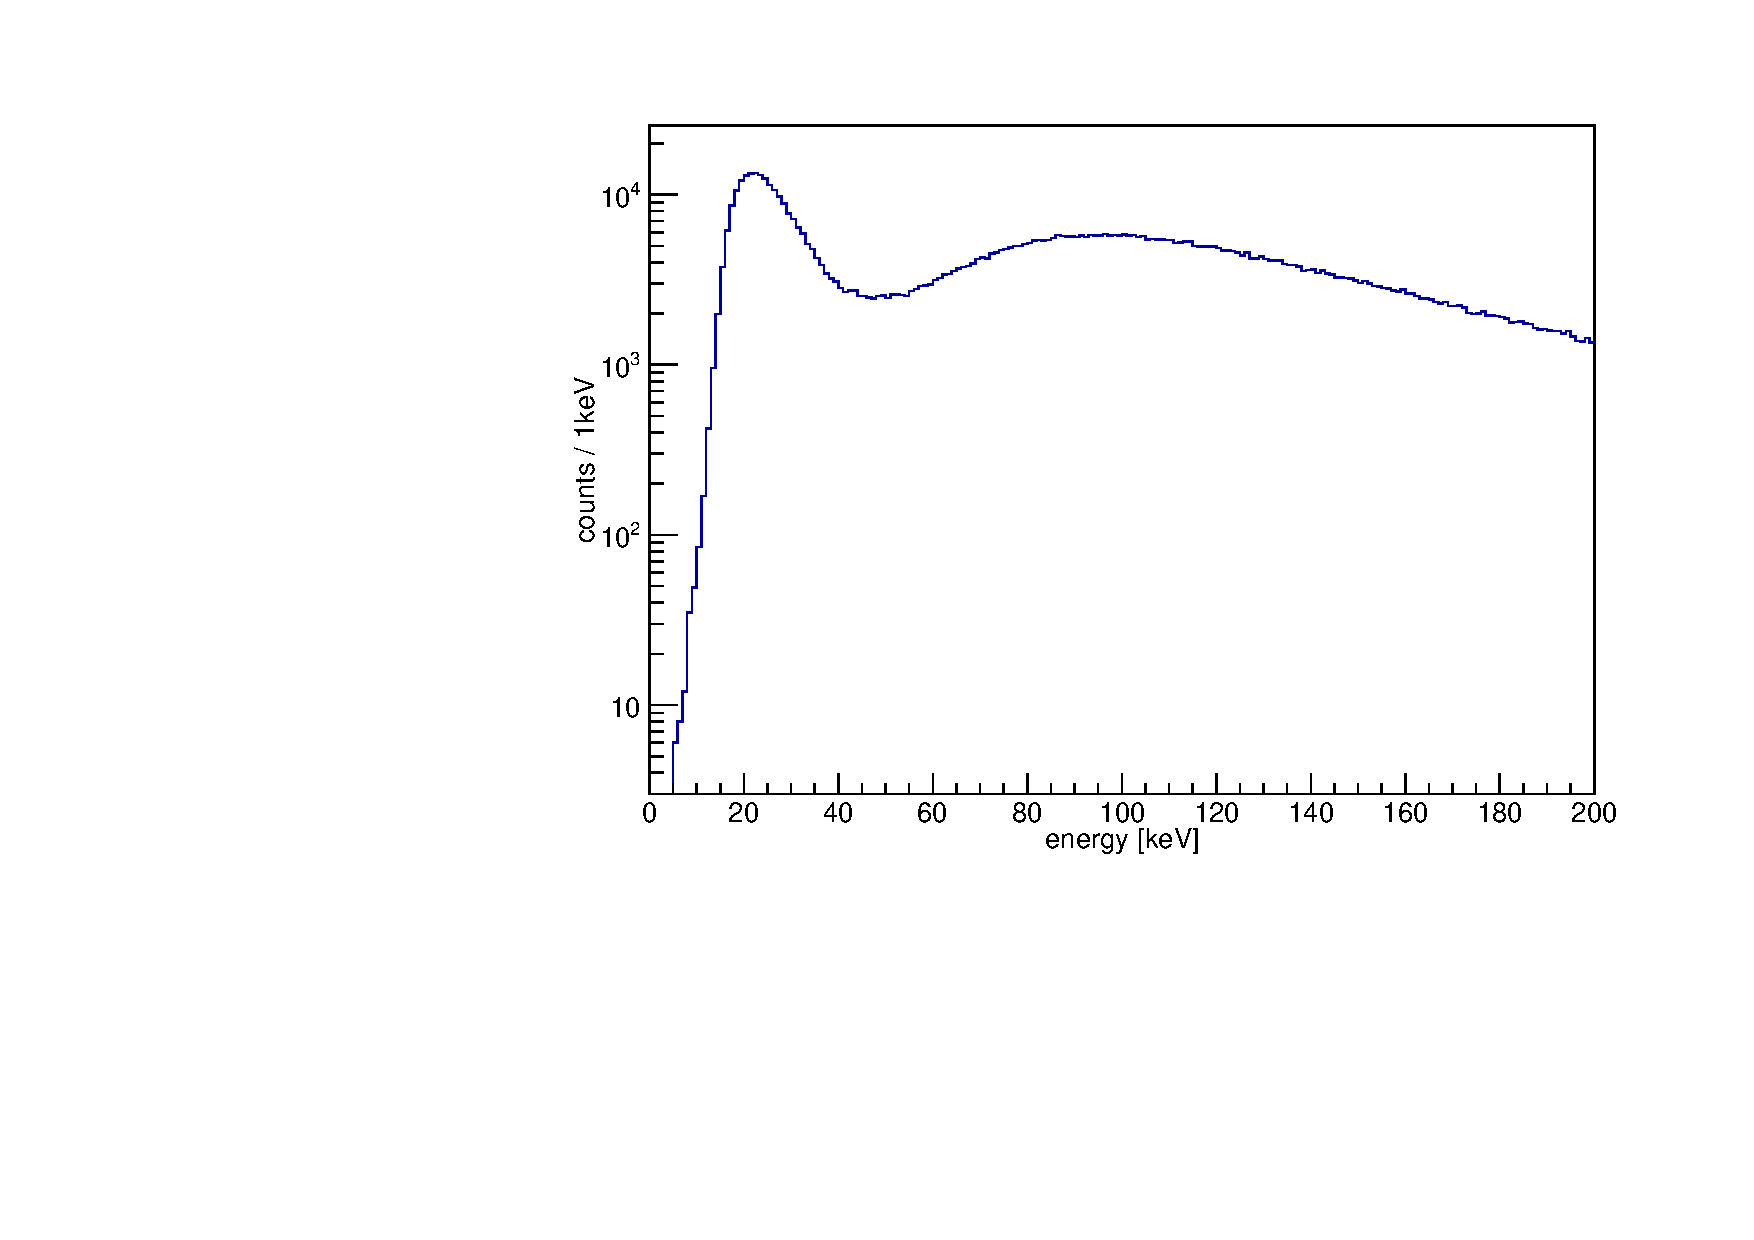
\includegraphics[width=\textwidth]{./Bilder/afterTheFall.pdf}
		\caption{after}
		\label{fig:after}
	\end{subfigure}
	\caption{
		Energy spectra from 0 to 200 keV. 
		Figure (a) shows the resulting spectrum of all events measured before the lowering of the lower energy threshold of recorded events on 12.10.2017 while (b) shows the spectrum after this date.
		}
		\vspace{5mm}
\end{figure}

The second discontinuous behavior originates from the same problem that was already faced in the line count rate analysis.
Not all detectors were on all of the time and time intervals occurred in which no signal at all was recorded.
Due to the fact that some of the detectors were turned on or off over the time of \PII\ will result in discontinuous changes in the event rate because of a change in detector efficiency over time.
This can easily be solved by only considering those events measured in a detector that was always turned on.
Which detector was always on over all of \PII\ can be seen in figure \ref in the appendix.
On the other hand due to there being time intervals in which no events were recorded the event rate drops discontinuous to zero there.
In section \ref{sec:CalcActiv} this problem was solved by calculating an effective measuring time for each detectors.
Her, however, an average measurement time over the entirety of \PII\ is of interest.
In this method we must find a way to weigh each individual bin of the event histogram with the corresponding effective measurement time of that bin.
This is where the test pulse signal comes in handy again.
Similar to the first method one can now determine an effective measuring times for each time interval of the bins of histogram \ref{fig:ZeitLimits}.
These mean measuring times can easily be calculated by plotting the test pulse signals in an histogram with the same binning as the event histogram and dividing each of these bins with the frequency of the test pulse of $f_\mathrm{TP} = 0.05\unit{Hz}$ (see figure \ref{fig:effectiveMeasuringTimes}).
The contents of these bins in the test pulse histogram correspond now to the respective measuring time in the binning intervals. 
\\

By dividing all bins of histogram \ref{fig:ZeitLimits} by the corresponding bins in the test pulse histogram, you would get a new histogram showing the mean count rate in each time frame of the bins (see figure \ref{fig:ChangeInEventRate}).
\\
\begin{figure}[t!]
	\centering
	\begin{minipage}[t]{.475\textwidth}
		\centering
		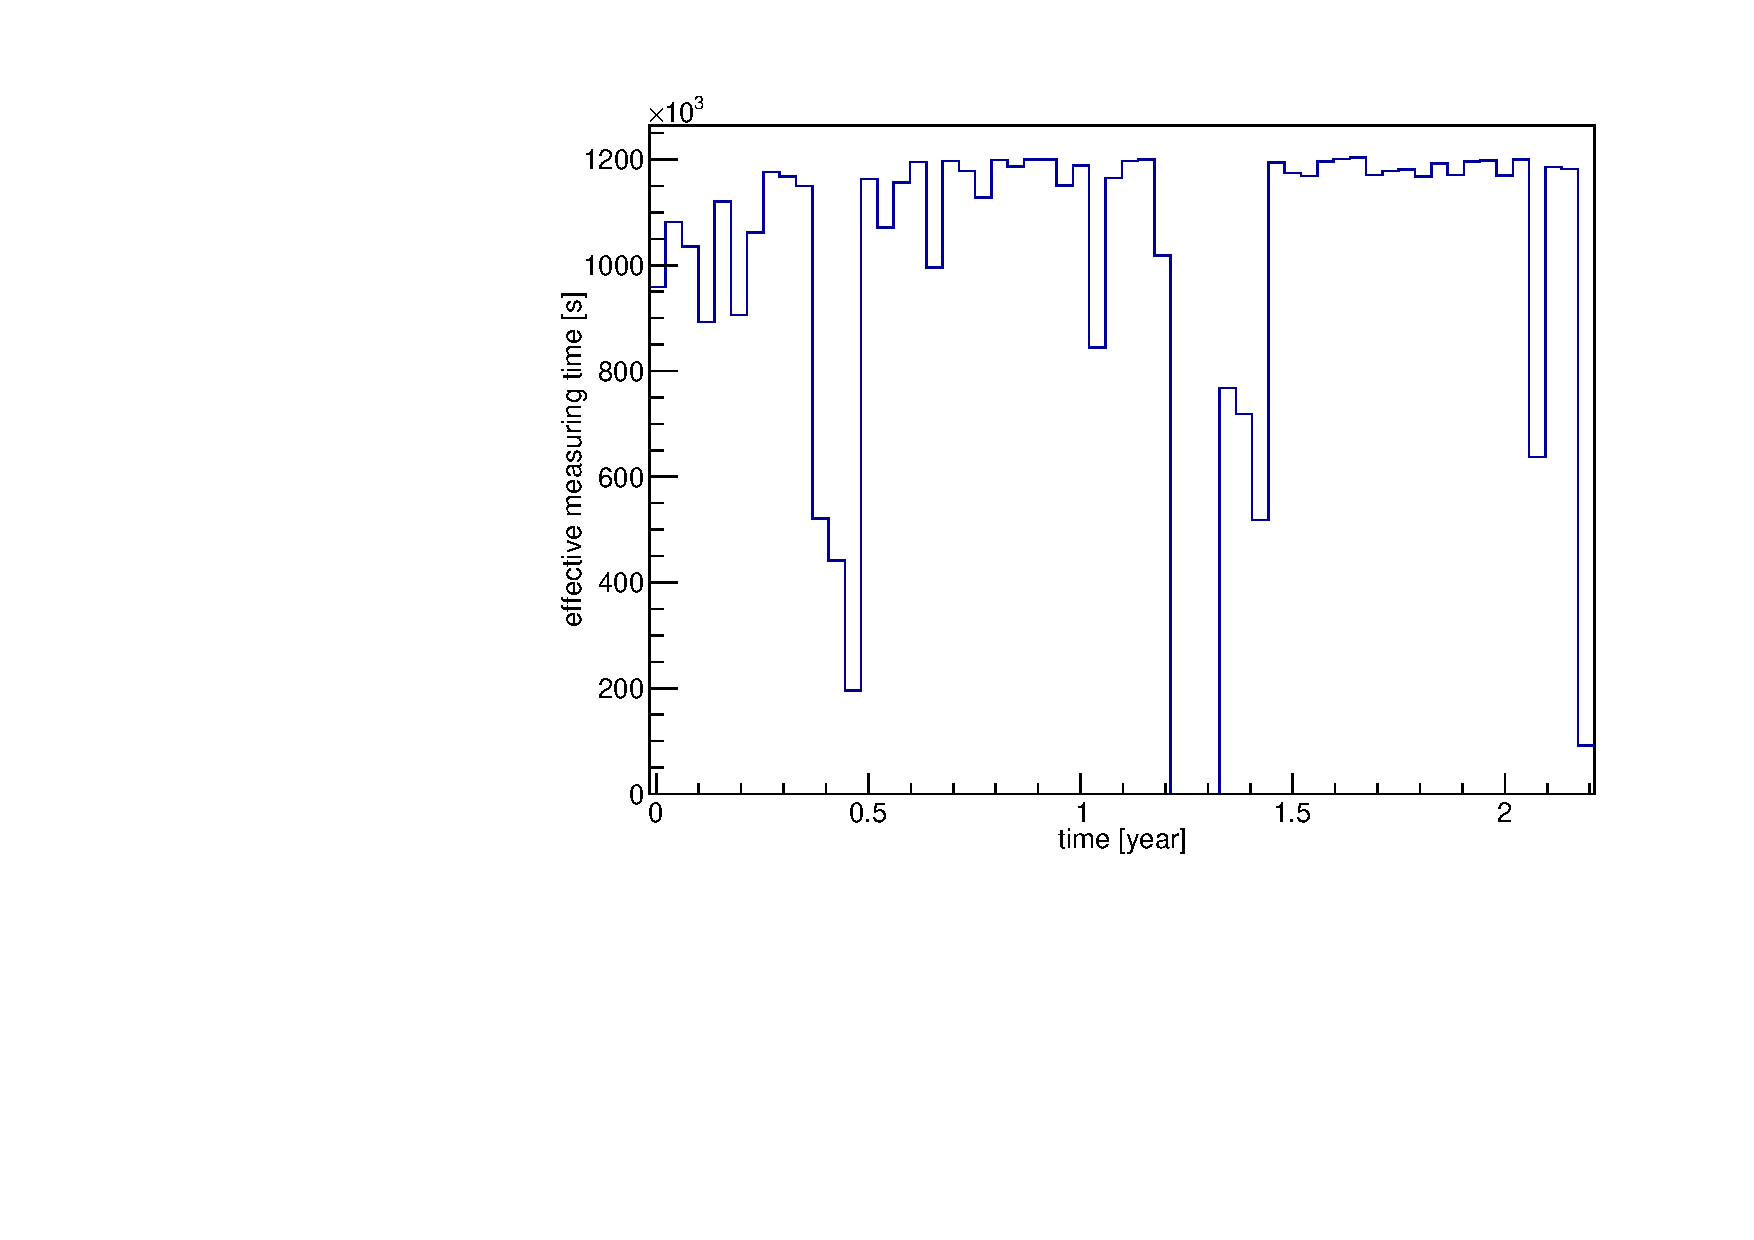
\includegraphics[width=\textwidth]{./Bilder/testpuler.pdf}
		\caption{
			Histogram showing the mean measuring time of each week corresponding to the individual bins.
			Those were determined by the amount of test pulse signals measured in the time frames and their amount multiplied by 20s.
			One can see, that the measuring time of each week varied on a broad level.
			}
		\label{fig:effectiveMeasuringTimes}
	\end{minipage}\hfill%
	\begin{minipage}[t]{.475\textwidth}
		\centering
		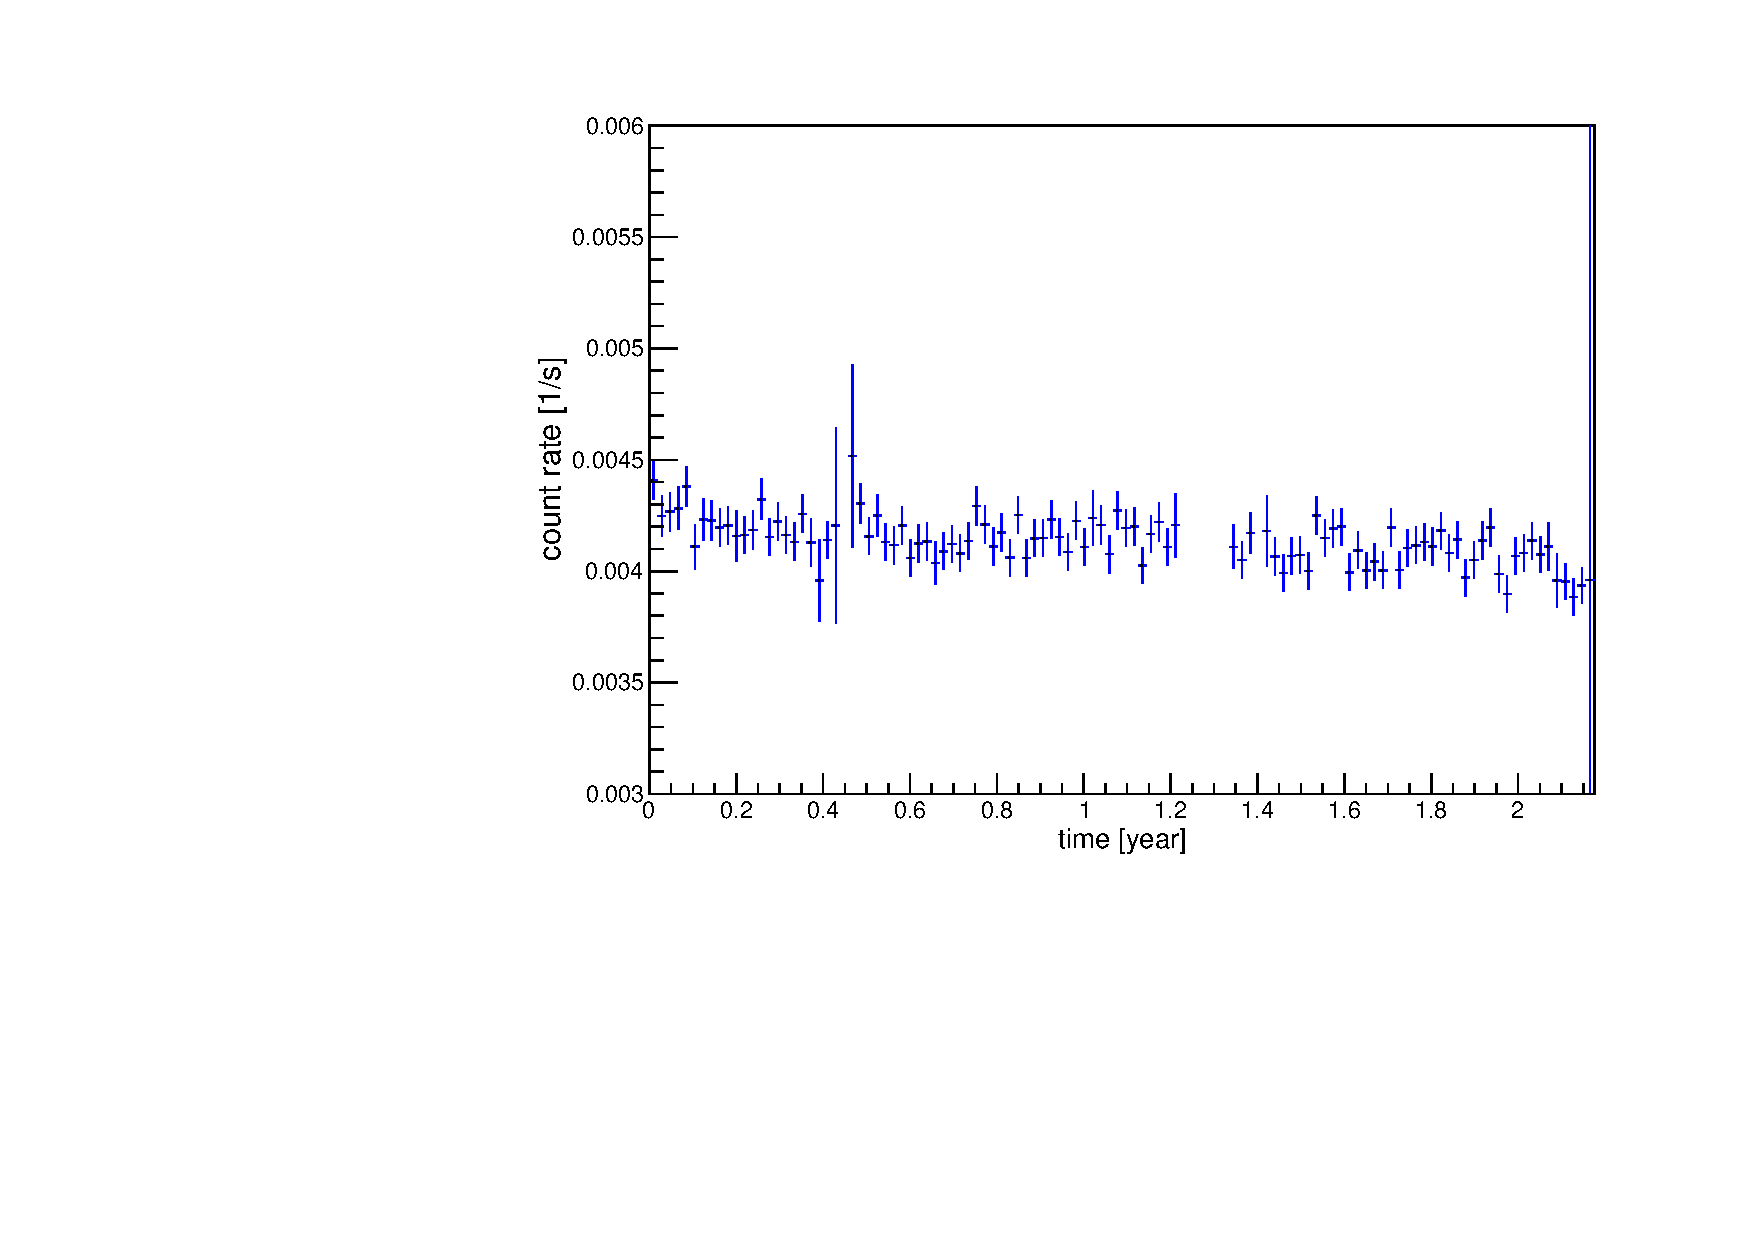
\includegraphics[width=\textwidth]{./Bilder/eventRate.pdf}
		\caption{
			Count rate of measured events between 200 and 400 keV over the course of \PII.
			A continuous change in rate can be seen. 
			One can now apply a fit using function \ref{equ:FitFilters2} and through it determine the count rate of \Kr\ at the start of \PII.
			}
		\label{fig:ChangeInEventRate}
	\end{minipage}
	\\
\end{figure}

From this graph one can now determine the exponential change in the event rate by applying an exponential fit function.
The fit function used here is
\begin{equation}
\mathrm{f}(x) = \mathrm{A}\times\exp\left(-\frac{\log(2)}{\mathrm{B}} x \right) + \mathrm{C}
\label{equ:FitFilters2}
\end{equation}
In this A corresponds to the initial count rate caused by \Kr\ decays, B to \Kr's half life and C the constant background rate.
By assuming that only \Kr\ has a notable change over time fit-parameter B was fixed to \Kr's half life \(10.739\unit{y}\) and leaving the other two parameter relatively free.
From the resulting fitting plot (seen figure \ref{fig:ChangeInEventRateFit}) one gets the fit parameters as seen in table \ref{tab:FitParZeit}.
The only parameter needed for the further analysis is parameter \(\mathrm{A}\) being the initial count rate $R_{\mathrm{count}} = (1.560\pm1.022) \unit{mHz}$ wanted from the fitting process. 
Now that the \Kr\ count rate has been determined all that is still needed to calculate \Kr's specific activity is the conversion factor from the measured events to the necessary \Kr\ decays in the LAr to cause the measured \Kr\ count rate.
As described above a new Monte Carlo simulation is needed for that.
What this simulation actually simulates and how one determines the conversion factor from it is the topic of the following section.


\begin{table}[t!]
	\centering
	\begin{tabular}{|l|c|}
		\hline
		Name 	& Value  \\ 
		\hline
		A [1/s] &	(1.521 $\pm$ 0.224)$\times10^{-3}$\\	
		\hline
		B [yr] &	10.739\\	
		\hline
		C [1/s] &	(2.714 $\pm$ 0.210)$\times10^{-3}$\\
		\hline
	\end{tabular}
	\caption{
		Fit parameters of fit function \ref{equ:FitNoFilters} applied on the spectra of the respective detectors.
		Parameter A represents the amplitude of the exponential decay function and B the half life of the decaying isotope.
		fit parameter C is there to handle the constant background created by other radioactive isotopes with much higher half lives.
		}
    \label{tab:FitParZeit}
\end{table}

\begin{figure}[t!]
	\centering
	\ifmakefigures%
	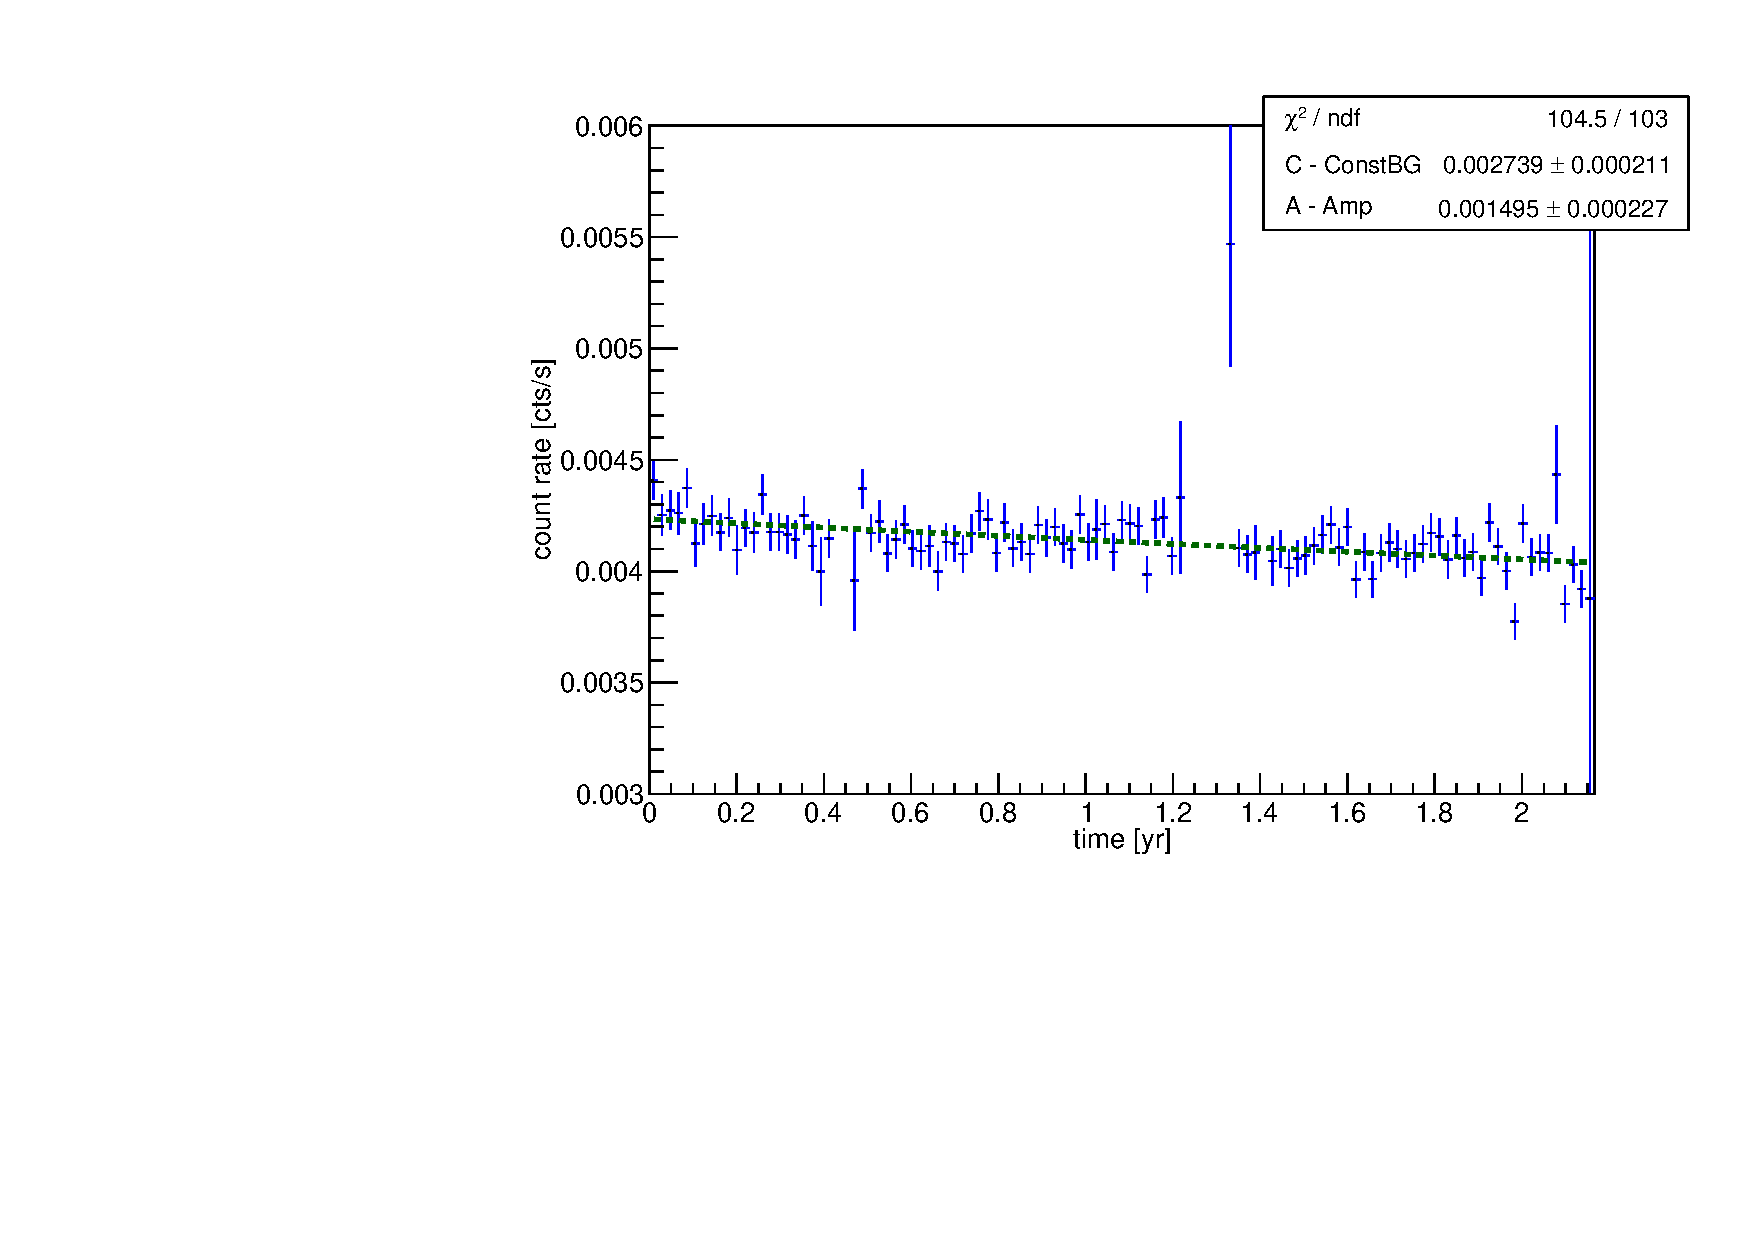
\includegraphics[width=100mm]{./Bilder/eventRateFit.pdf}
	\fi%
	\caption{
	    Fitted count rate diagram over the time frame of \PII.
	    For the fitting process function \ref{equ:FitFilters2}.
	    The resulting fit parameter can be seen in table \ref{tab:FitParZeit}.
	}
	\label{fig:ChangeInEventRateFit}
\end{figure}%


To calculate this conversion factor one basically has to apply the same process as in the line count rate analysis.
Just this time one does not just simulate the emission of photons with an energy of 514keV in the LAr.
One rather simulates the actual \Kr\ decays themselves.
A problem however is, that one can expect the detector efficiency of \Kr\ to be very small.
This is due to the fact that electrons being created in the LAr have a low probability of being measured .

On the one hand, electrons emitted far away from the detectors have a longer distance to travel in which they lose a lot of energy by generating scintillation light, effectively reducing their range.

On the other hand, electrons only have a small transmission factor in germanium.
This causes the problem that a significant number of them are detected in the dead zone of the detectors where they do not generate measurable signals.
In comparison, photons have a larger transmission factor that allows them to deposit their energy deep in the active volume of the detectors.

It must also be taken into account that only those events are used in the further analysis that have made their signal in one of the detectors that was always on.
Every other decay that made a signal in another detector will be discarded making the detector efficiency even smaller. 
Because of this low expected detector efficiency a much higher amount of decays have to be simulated than in the case of the first Monte Carlo simulation.
\\
\begin{figure}[t!]
	\centering
	\begin{minipage}[t]{.475\textwidth}
		\centering
		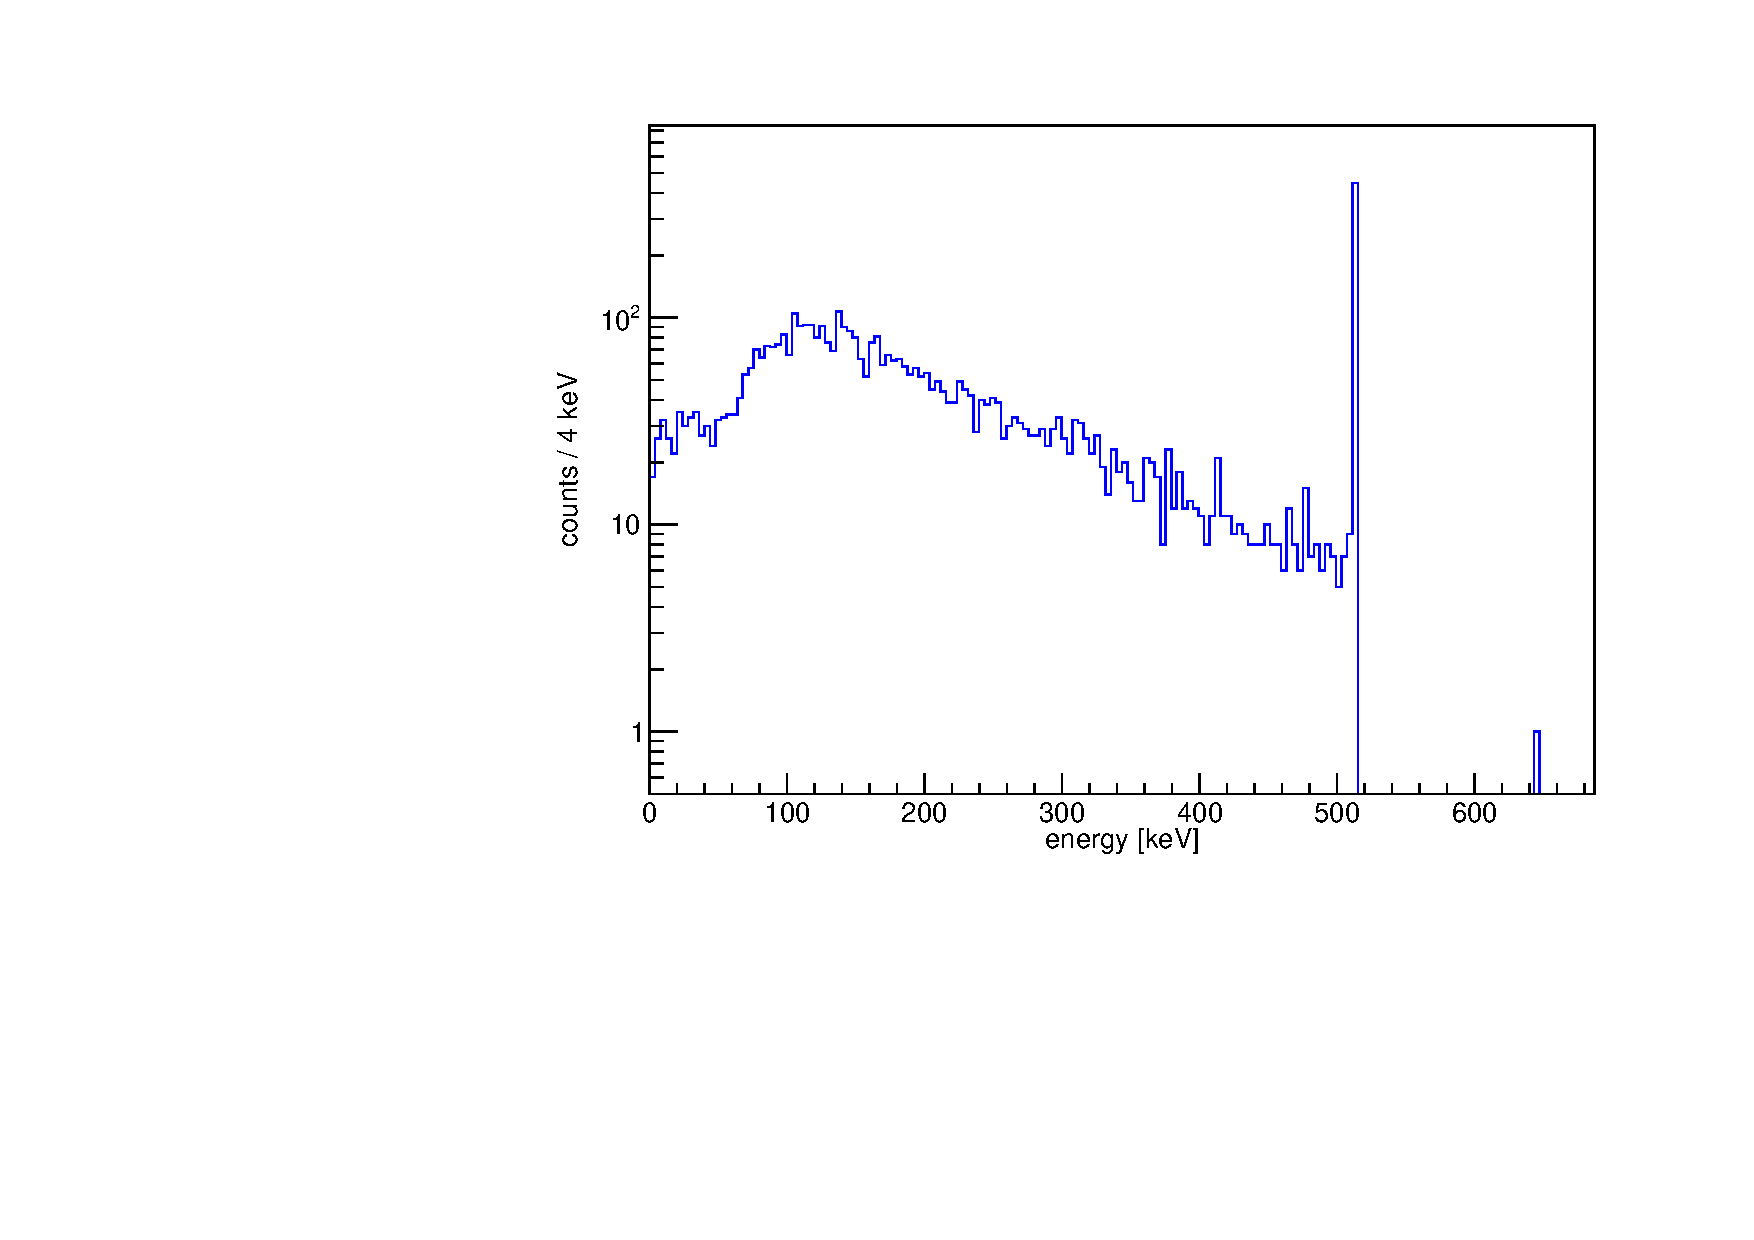
\includegraphics[width=\textwidth]{./Bilder/Sim1Phasenraum.pdf}
		\caption{
			Energy spectrum computed by simulating 1 billion \Kr\ decays and plotting the counts of events by their corresponding energy.
			The blue colored area represents the amount of counts used for the calculation of the detector efficiency.
			From it can be seen, that the majority of events were created by the photons of the 514 keV peak and only about 20$\%$ from the electrons of every other \Kr\ decay.
			}
		\label{fig:Sim1Spektrum}
	\end{minipage}\hfill%
	\begin{minipage}[t]{.475\textwidth}
		\centering
		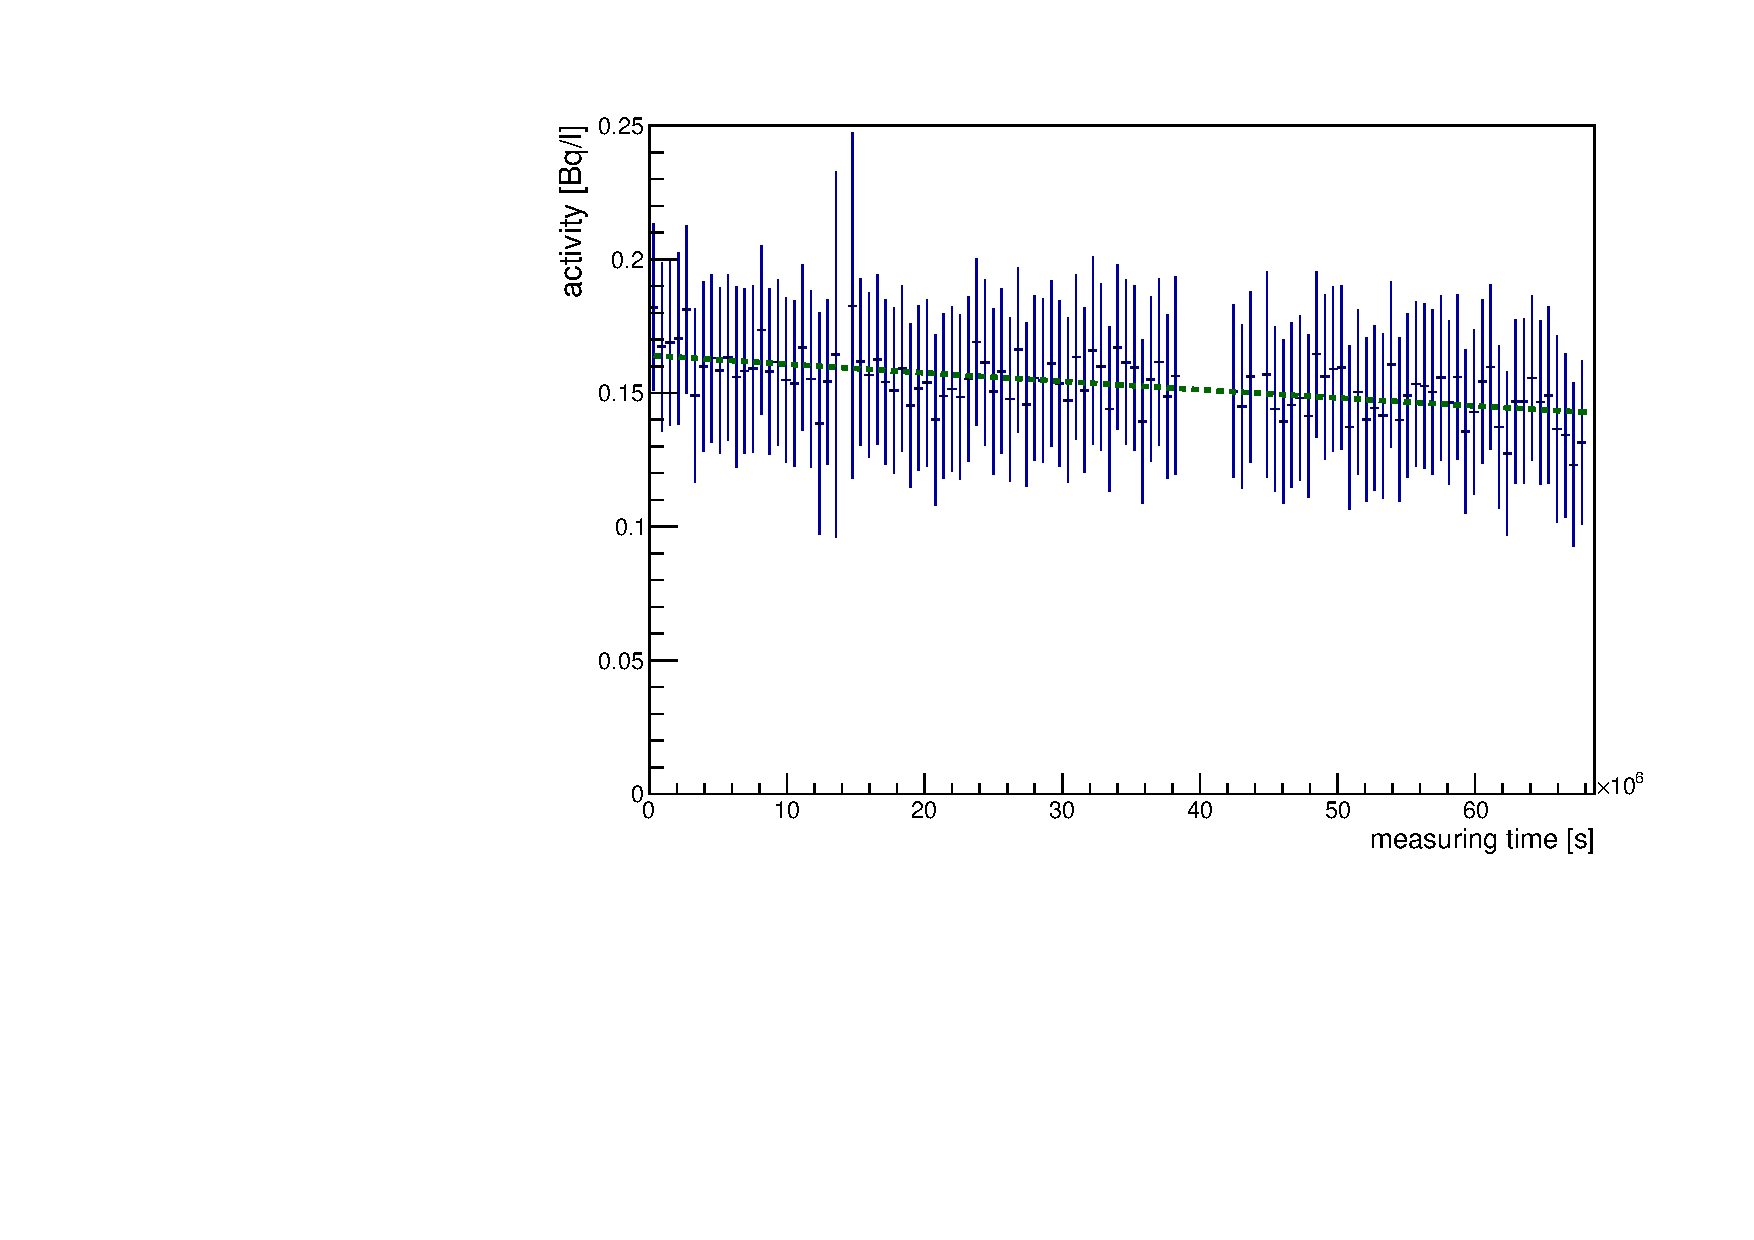
\includegraphics[width=\textwidth]{./Bilder/Aktivitaet.pdf}
		\caption{
		The calculated specific activity of \Kr\ over the time frame of \PII.
		This plot was created by subtracting the constant background of each point in figure \ref{fig:ChangeInEventRateFit} and multiplying each value with the conversion factor.
		}
		\label{fig:activity}
	\end{minipage}
\end{figure}

\section{Monte Carlo simulation}
\label{sec:MonteCarlo2}

That is why a number of N = 1 billion \Kr\ decays in a volume of again $V_{sim} = 17.65 \mathrm{m}^3$ was simulated.
Due to the massive amount of these simulated events only those decays were saved in which a signal has actually been measured.
These events created a combined spectrum of the emitted electrons plus the photons emitted from the excited \nuc{Rb}{85m} as seen in figure \ref{fig:Sim1Spektrum}.
If you compare this spectrum with the one determined for the other Monte Carlo simulation you can see these two spectra look relatively similar.
To test this one can calculate a ratio from the two spectra and compare them.
An appropriate ratio for the range of values of this analysis would be to take the sum of all events with an energy between 200 and 400 keV $N_{\mathrm{sum}}$ and divide by the counts in the 514 keV peak $N_ {\mathrm{peak}}$.
This results in a value of $N_{\mathrm{sum}}/N_{\mathrm{peak}} = 2.481$ for the first simulation and $3.137$ for the second simulation.
Due to the fact that the first simulation only computed 514 keV photons the first value represents the ratio when only the 514 keV photons would contribute to the energy spectrum.
The second value, on the other hand, represents the ratio when the 514 keV photons together with the electrons generate the spectrum.
This means that the electrons only generate about 20$\%$ of all measured events in the range of 200 to 400 keV.
The 514 keV photons created the rest.
\\

This is actually an advantage.
If the majority of the measured events were created by electrons then one would have to apply a correction onto the detector efficiency.
This is because of a weakness of the simulated detectors.
The dead layer of the actual detectors isn't known that well which is why the simulated detectors can only work with an assumptions of the actual dead volume of the detectors.
Unfortunately, it's hard to correct the determined value for this weakness.
It is therefore lucky that the 514keV photons are responsible for the majority of counts in the spectrum and no such correction has to be applied.
\\

But this conclusion of photons being the main cause of the spectrum assumes that in both simulations the same environmental conditions and \Kr\ characteristics were simulated.
Whether this is true or not can easily be determined by looking at line count of the characteristic 514keV peak.
In the case of the first simulation an amount of 10179 events were measured by the BEGe detectors in the 514keV peak with a decay density of about 2832 $\unit{photon}/\unit{l}$.
On the other hand in the second simulation only 817 events were measured with a decay density of 56640$\unit{decay}/\unit{l}$.
But one has to consider that in the case of the first simulation only the photons of the \nuc{Rb}{85m} relaxation were emitted and \Kr\ only decays into this exited state with a probability of 0.434$\%$.
The effective decay density of the first simulation is therefore about 652511 $\unit{decay}/\unit{l}$.
To compare these two line counts, one now has to scale one of the two line counts so that the same decay density can be assumed.
By applying the scale of $\frac{56640}{652511}$ onto the amount of events in the 514keV peak from the first simulation you get a adjusted value of 884 events.
The fact, that this value is roughly the same size as the value 817 form the second simulation, proves, that a similar environmental situation and \Kr\ characteristics must have been simulated.
This conclusion also justifies retroactively the simplification in the first simulation where only photons of the \nuc{Rb}{85m} were emitted to replace the computation of the actual decays.
\\

Now to calculating the conversation factor from this simulation.
This requires determining the number of events with an energy in the range 200 to 400 keV and the untriggered detector anticoincidence veto.
In this case an amount of $\Delta N$ = (1438$\pm$38) events was determined.
With the absolute amount $N_{\mathrm{sim}}$ of decays simulated we determine a detector efficiency of
\begin{equation*}
    \epsilon = \frac{\Delta N}{N_{\mathrm{sim}}} = (1.438\pm0.038)\times10^{-6} \frac{\unit{event}}{\unit{decay}}
\end{equation*}
This values says that any decay in the liquid argon has a probability of $\epsilon$ to be measured by one of the detectors that was always on.
With this value one can again calculate the volume independent conversation factor
\begin{equation*}
    \frac{1}{\epsilon V_{\mathrm{sim}}} = (39.38\pm1.04) \frac{\unit{decay}}{\unit{event} \times \unit{l} }
\end{equation*}
With this conversation factor one can now finally calculate the specific activity of \Kr.
By applying equation \ref{equ:ActivityDieZweite} and feeding it with the values found we result in an specific activity of $a(t=0) = (61.4\pm41.9) \frac{\unit{mBq}}{\unit{l}}$ at the start of Phase II.

One can now get back to the graph \ref{fig:ChangeInEventRateFit}, subtract the constant background of each point and scale each value by the conversation factor.
The resulting graph can be seen in figure \ref
Now it is of interest to compare this value to the specific activity found in the line count rate analysis.
For this one has to calculate the mean specific activity over all of Phase II.
This can easily be done by integrating an exponential decay function over all of \PII\ and then dividing it by 2.17 yr.

\begin{equation*}
    \bar{a} = \frac{1}{2.17\unit{yr}} \int_0^{2.17\unit{yr}} a(t=0)\times\exp \left( \frac{\log(2)}{T_{\frac{1}{2}}} t \right) \mathrm{d}t
\end{equation*}

with $T_{\frac{1}{2}}$ being the half life of \Kr.
This results in an mean specific activity of $ \bar{a} = 57.294 \frac{\unit{mBq}}{\unit{l}}$.
\\

When comparing the here obtained result with the specific activity found in the line count rate analysis you will realize that there is a problem.
The mean specific activity of all investigated detectors found in the first method had a value of $\bar{a} = (0.508\pm0.086)\frac{\unit{mBq}}{\unit{l}}$.
Compared to this is the value determined here is two orders of magnitude bigger.
This is problematic.
The critical question are now: 
Which of the methods is faulty, which of the assumption used was wrong and can one still make a statement about \Kr\ specific activity from the problematic approach.
These question will be answers in the following section.
\\


\section{Discussion}
\label{Discussion}

The biggest advantage of the line count rate analysis compared to the second method is that in its case the investigated effect can only originate from \Kr\ and no other isotope.
Because of this the likelihood of its determined value being the actual specific activity is relatively high.
By comparing the results of the first method with those of the WARP and Darkside experiments, you have already seen that the specific activity of \Kr\ is lower than in all other experiments.
The second method however has the problem that theoretically every other isotope that is residual in the LAr contributes to the investigated change over time.
It can therefore be very likely that the mistakes made lies in the assumption that all contribution of any other isotope to this change can be ignored. 
In the beginning of this chapter all isotopes that are the most probable sources of error have already been discussed.
It was already concluded that any contributions from \nuc{Ar}{39} and \nuc{Po}{210} can be disregarded due to their either high half life or their high mean kinetic energy of the escaping particle.
But as it was already indicated there, it might be necessary to discuss the influence of \nuc{Ar}{42} further.
\nuc{Ar}{42} has a half life of 32.9 y which is in the same order of magnitude as the half life of \Kr.
thereforee, one can expect to see a change in its activity over the course of \PII~ of about 4.4$\%$ of its absolute specific activity.
With an specific activity big enough one could expect this isotope to be responsible for the measured decrease.
But due to \nuc{Ar}{42}'s specific activity being much lower than the measured amplitude of $57.294 \frac{\unit{mBq}}{\unit{l}}$  it can not be the only cause of this .
\\

What is really interesting about \nuc{Ar}{42}, is not the decay of \nuc{Ar}{42} itself, but rather its daughter nuclei \nuc{K}{42}.
\nuc{K}{42} has a half life of 12.355 h \cite{chen_nuclear_2016}.
It can now be approximated, that \nuc{K}{42}'s specific activity is equal to \nuc{Ar}{42}'s specific activity.
This comes from the fact that in comparison to the half life of \nuc{Ar}{42} the resulting \nuc{K}{42} practically decays instantaneously.
This means that it is possible to directly assign one \nuc{K}{42} decay to each \nuc{Ar}{42} that decays.
This doubles the number of decays which can be attributed to \nuc{Ar}{42}.
But assuming that the individual \nuc{Ar}{42} and \nuc{K}{42} isotopes are homogeneously distributed in the LAr, their combined specific activity is still by far not big enough to explain the bigger amplitude measured.
\\

But here lies the critical point.
The \nuc{K}{42} isotopes are in fact not homogeneously distributed in the LAr.
To understand why they are not one has to look at what a \nuc{K}{42} does right after it is formed.
Right after a \nuc{Ar}{42} decays its resulting \nuc{K}{42} isotope positively ionized.
This results from the fact that the newly formed electron escapes from the decay position due to its high velocity.
Now that the \nuc{K}{42} isotopes are positively charged, they can be deflected by an electric field.
\\

Such fields in the LAr tank originated from the germanium detectors.
In a germanium detector it is necessary to create a great electrostatic potential difference between the doped electrodes.
The resulting electric field separates electron-hole pairs that might have been created by other particles depositing their energy in the semiconductor \cite{spieler_semiconductor_2005}.
The field then guids the particles to the respective electrodes and by that creating a current which can be measured externally.
For a high detection efficiency strong fields are necessary.
Otherwise the electron or the hole might recombine in the p-type volume without creating any signal.
\\

The positively ionized isotopes are now deflected by these electrostatic fields to the negatively charged surface of the detectors. 
In the LAr the mean time it takes the ionized \nuc{K}{42} to capture an electron as compensate for its positive charge is relatively long. 
Thats why even though the fields are not very strong far away of the detectors the \nuc{K}{42} can still travel a relatively long distance before it either captures an electron or decays itself. 
Now that the density of \nuc{K}{42} isotopes is higher near the germanium detectors it can be expected that the specific activity around the detector also increases.
\\

The effect explained here has already been measured in \gerda\ and it is actually one of the greatest background sources of the whole experiment.
\nuc{K}{42} has also the unfortunate characteristic for the \gerda\ experiment that its Q-value of about $Q_\beta =3525\unit{MeV}$ lies higher than the Q-value of the double beta decay of \nuc{Ge}{76} $Q_{\beta \beta} = 2039\unit{MeV}$.
This means that electrons of the \nuc{K}{42} decay can create background events in the investigated rage. 
Initially it was not expected to create much background.
Its influence on the measurement however was only recognized after the start of \PI, when its counting rate was higher by a factor of 20. \cite{becerici_schmidt_results_2014}.
Techniques to suppress the background of \nuc{K}{42} were introduced over time like the usage of nylon mini-shrouds (NMS) as a mechanically barrier.
The NMS together with the active filters of the pulse shape analysis and the LAr veto have proven to bee able to suppress \nuc{K}{42} events by more then three orders of magnitude.
\\

In this case however it is not possible for the analysis to use the active filters to suppress the \nuc{K}{42} further.
Otherwise one would also filter out the \Kr\ events that are supposed to be investigated here in the first place.
So it still can be expected that a not negligible proportion of the measured specific activity comes from the denser \nuc{K}{42} in the region of the detectors.
What effective specific activity can be expected from the \nuc{Ar}{42} is difficult to estimate, but you can assume that it should be far greater than that of \Kr.
To get a quantitative approximation, you can use the plot of the event rate change again (see \ref{fig:ChangeInEventRate}) and modify the fit function used so that two exponential decays plus a constant background are taken into account.
Both exponential decay fit functions have their half life fixed to the respective values of \Kr\ (10.739y) and \nuc{Ar}{42} (32.9y).
The used fit function can be seen in equation \ref{fig:doubleFitFun}, the resulting fit function in figure \ref{fig:double} and the fit parameter in table \ref{tab:doubleFitpara}.
\begin{equation}
    \mathrm{f}(x) = \mathrm{A}\times\exp\left(-\frac{\log(2)}{\mathrm{B}} x \right) + \mathrm{C}\times\exp\left(-\frac{\log(2)}{\mathrm{D}} x \right) + \mathrm{E}
    \label{equ:doubleFitFun}
\end{equation}

\begin{table}[t!]
	\centering
	\begin{minipage}[t!]{.475\textwidth}
	\centering
	\ifmakefigures%
	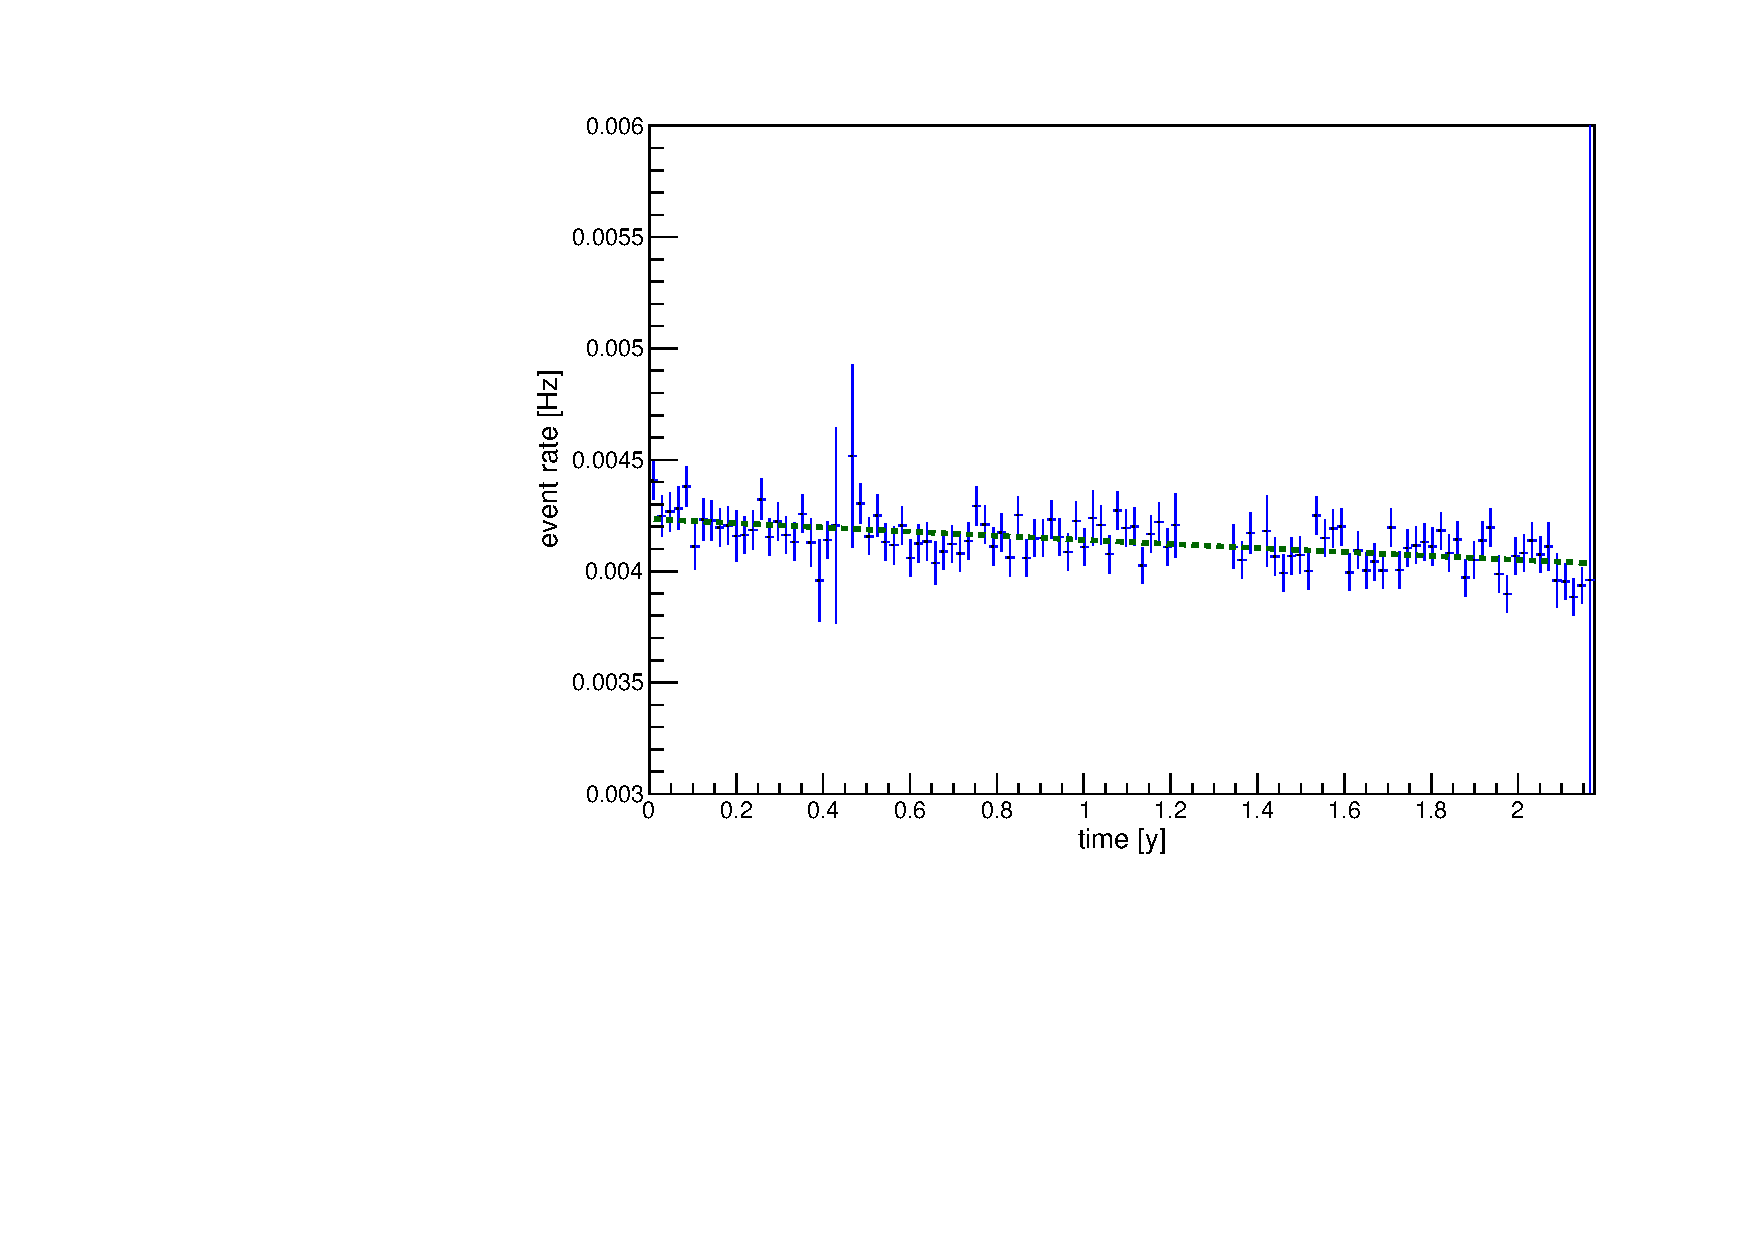
\includegraphics[width=75mm]{./Bilder/doppelt.pdf}
	\fi%
	\captionof{figure}{
		    Fitted count rate diagram over the time frame of \PII.
	    For the fitting process function \ref{equ:doubleFitFun}.
	    The resulting fit parameter can be seen in table \ref{tab:doubleFitpara}.
	}
	\label{fig:double}
	\end{minipage}\hfill%
    \begin{minipage}[t!]{.475\textwidth}
    \centering
    \begin{tabular}{|l|c|}
        \hline
        Name  & Value \\
        \hline
        A [1/s]    & (1.024$\pm$0.122)$\times 10^{-3}$ \\
        \hline
        B [yr] & 10.739 \\
        \hline
        C [1/s]  & (1.454$\pm$0.130)$\times 10^{-3}$ \\
        \hline
        D [yr] & 32.9 \\
        \hline
        E [1/s] & (1.757$\pm$0.120)$\times 10^{-3}$ \\
        \hline
    \end{tabular}
    \caption{
        Fit parameters of fit function \ref{equ:FitNoFilters} applied on the spectra of the respective detectors.
		Parameters A and C represent the amplitude of the exponential decay function and B and D the half lives of the decaying isotopes.
		Fit parameter E is there to handle the constant background created by other radioactive isotopes with much higher half lives.
    }
    \label{tab:doubleFitpara}
	\end{minipage}
\end{table}


In a direct comparison of figure \ref{fig:double} with graph \ref{fig:ChangeInEventRateFit} no real difference can be see.
When looking at the fit parameters however one can see that in this case the \nuc{Ar}{42} exponential fit function has a bigger amplitude than \Kr.
Because the \nuc{K}{42} density is not homogeneously distributed in the liquid argon it is impossible to run a Monte Carlo simulation to again determine a new detector efficiency.
But using the conversation factor determined from the second simulation to make an estimate the respective effective specific activities can be calculated to $(40.4\pm0.59)\frac{\unit{mBq}}{\unit{l}}$ for \Kr\ and $(57.3\pm0.66)\frac{\unit{mBq}}{\unit{l}}$ for all of the decays resulting from \nuc{Ar}{42}.
These values are both still way to high for what was expected of them.
The maximum effective specific activity of \nuc{Ar}{42} expected to be  only about one orders of magnitude higher than the actual specific activity of only the \nuc{Ar}{42}.
But due to the fit parameters still generating far too much specific activity for these isotopes shows that other sources of change are still not accounted for.
\\

Nevertheless it has been shown with this fit that \Kr\ does not contribute solemnly to the change of count rate over time and with this the assumption from before has been shown to be false.
It would still be possible to determine an specific activity of \Kr\ from plot \ref{fig:ChangeInEventRate} by considerein every individual source of change in count rate.
But due to the higher number of fit parameters that would have to be determined and the way to small time frame compared to the half lifes of the isotopes, one can be quite pessimistic whether this analysis can even make a satisfying statement about the specific activity of \Kr.
\\

At the end of this analysis it is of interest again to investigate how the change in the count rate would have looked over time if the specific activities of the WARP or the Darkside experiment had been present.
Again, in the case of the WARP experiment an activity of $(0.16\pm0.13)\frac{\unit{Bq}}{\unit{l}}$ was measured. 
If one would plot its equivalent amplitude in a diagram like Figure \ref{fig:ChangeInEventRateFit} a significant change would have been visible.
On the other hand is the activity in the Darkside experiment with its $(2.8577 \pm 0.18122) \frac{\unit{mBq}}{\unit{l}}$ too small to measure an apparent change over time.
\\



% use fit to calculate the decrease in rate of the signals in range from 200 to 500keV
% from fit and assumption that only Kr85's activity is decreasing one can calculate the specific activity from the amplitude of the fit

% use Volume of LAr-Tank to determine the number of Kr85 and from this the concentration in the argon

\chapter{Summary and Outlook}
\label{sec:ConcAndOutlook}
\section{Summary}
With the line count rate analysis carried out in this paper it was able to show that the specific activity of \nuc{Kr}{85} in the LAr in \gerda\ \PII\ has a value of $(0.508\pm0.086) \frac{\unit{mBq}}{\unit{l}}$. 
Compared to WARPs $(160\pm130)\frac{\unit{mBq}}{\unit{l}}$ and to Darksides $(2.8577 \pm 0.18122) \frac{\unit{mBq}}{\unit{l}}$ its value is much smaller.
On the other hand, the second attempt to determine a value for the specific activity via the change of count rate over time has failed.
This was due to the falsely made assumption that \Kr\ is the only isotope in the LAr to show significant change in its activity over time.
\\
\section{Comparison to WARP and Darkside}

One can now make some comparisons of this value with the WARP and the Darkside experiments.
In the case of the WARP experiment a specific activity of $(160\pm130)\frac{\unit{mBq}}{\unit{l}}$ \label{} was measured for the \Kr.
On the other hand, an specific activity of $(2.8577 \pm 0.18122) \frac{\unit{mBq}}{\unit{l}}$ was measured in the Darkside experiment.
The here determined value of $(0.508\pm0.085)\frac{\unit{mBq}}{\unit{l}}$ is about one order of magnitude smaller than the specific activity in the Darkside and whole three orders of magnitude smaller than the WARP experiment.
From these comparisons one can see, that the specific activity of \Kr\ in \gerda\ \PII\ seems to be much smaller than in other experiments using LAr.
\\

What one can also do is take the specific activities of the other two experiments and determine how many counts one would have been able to measure if the \Kr\ had their specific activity.
As simplification only the theroeticall values for the BEGe detectors was determined. 
How many counts the corresponds activity would induce in the BEGe detectors can be determined with the help of formula \ref{equ:correspondingEvents}.
\begin{equation}
\mathrm{N} = \bar{a} \times p \times \epsilon_\mathrm{BEGe} V_{\mathrm{sim}} \times \bar{t}
\label{equ:correspondingEvents}
\end{equation}
With the activity and the values determined from the analysis above one can calculate a corresponding amount of about 76152 events for the WARP experiment.
In the case of the WARP experiment one could expect the count rate to be much higher than the 183 events determined from the actual measurement.
For the Darkside experiment with an amount of 1360 counts is again about one order of magnitude higher than the here measured events.
From these comparisons one can see that for a much higher specific activity of \Kr\ to have actually been present a much bigger amount of events should have been counted.
As a graphical representation, the peaks that would have been able to be seen in the measured spectrum are displayed in figure \ref{fig:WARP} and \ref{fig:Darkside}.
\\


\section{Outlook}
As it was mentioned in the introduction, the \gerda\ experiment is planned to keep measuring until 2020.
Afterwards the \gerda\ setup will be converted to the LEGEND experiment - a collaboration between the \gerda\ and the MAJORANA experiments.
There LAr is used again as coolant, but new argon is added which might again lead to a higher concentration of \Kr\ depending on where the argon was taken from.
LEGEND will also feature a new and more precise LAr veto setup.
With this new LAr veto it might  actually be possible to use the pre-coincedences of the \Kr\ decay in the line count rate analysis which would make a fitting of the peak possible. 
\\

Due to the comparably small specific activity of the \Kr\ in the argon it might be of interest to find out where it originated from.
As seen from other experiments as WARP \Kr\ can cause an non insignificant amount of background in the lower energy area.
For experiments interested in this region like the search for sterile neutrinos or dark matter in the energy range of keV this isotope might be a problematic isotope.
This might be prevented by finding out where the argon in \gerda\ \PII\ came from and why its \Kr\ concentration is so low there.
The argon from this area might be better suited for such low-background experiments.




%%%%%%%%%%%%%%%%%%%%%%%%%%%%%%%%%%%%%%%%%%%%%%%%%%%%%%%%%%%%%%%%%%%%%%%%%%%%%%%%
% -----------------------------------------------  ADD SOME ACKNOWLEDGMENTS  ---
%%%%%%%%%%%%%%%%%%%%%%%%%%%%%%%%%%%%%%%%%%%%%%%%%%%%%%%%%%%%%%%%%%%%%%%%%%%%%%%%
\newpage
\section*{Acknowledgments}

%%%%%%%%%%%%%%%%%%%%%%%%%%%%%%%%%%%%%%%%%%%%%%%%%%%%%%%%%%%%%%%%%%%%%%%%%%%%%%%%
%%%%%%%%%%%%%%%%%%%%%%%%%%%%%%%%%%%%%%%%%%%%%%%%%%%%%%%%%%%%%%%%%%%%%%%%%%%%%%%%

%----------------------------------------------------------------- appendix ----
%%%%%%%%%%%%%%%%%%%%%%%%%%%%%%%%%%%%%%%%%%%%%%%%%%%%%%%%%%%%%%%%%%%%%%%%%%%%%%%%
% --------------------------------------------------- ADD APPENDIX (IN CASE) ---
%%%%%%%%%%%%%%%%%%%%%%%%%%%%%%%%%%%%%%%%%%%%%%%%%%%%%%%%%%%%%%%%%%%%%%%%%%%%%%%%
\appendix

\section{Determining the resolution of the detector types}
\label{sec:ResDetermination}
rgdagadgadgdsgdsgrsgserg



% \section{}
% \label{}

%--------------------------------------------------------------- references ----
\backmatter

\bibliographystyle{plain}
\bibliography{references}
\listoffigures
\listoftables

\end{document}
